\chapterimage{Pictures/chap07/checkerboard-ref-465x930.png}
\chapter{采样与重构}\label{chap:采样与重构}
\setcounter{sidenote}{1}
尽管像pbrt那样的渲染器最终输出的是彩色像素的2D网格,
但实际上入射辐射是定义在胶片平面上的连续函数。
从该连续函数计算出离散像素值的方法会显著影响渲染器生成的最终图像的质量;
如果没有仔细执行该过程,则会出现伪影\sidenote{译者注:原文artifact。}。
反之,如果执行得很好,则为此进行相对少量的额外计算就能极大提升渲染图像的质量。

本章从介绍\emph{采样理论}开始——即从定义在连续域上的函数
取出离散样本值并用它们重建与原本类似的新函数的理论。
在采样理论和低偏差点集(一种均匀分布的样本点类型)思想的基础上,
本章定义的\refvar{Sampler}{}以不同方式生成$n$维样本向量
\footnote{回想上一章中\refvar{Camera}{}用\refvar{CameraSample}{}
在胶片平面、透镜上以及时间域中取点——通过取用这些样本向量前几维来设定\refvar{CameraSample}{}值。}。
本章将介绍五种\refvar{Sampler}{}实现,涵盖了采样问题的各种方法。

本章以类\refvar{Filter}{}和\refvar{Film}{}作结。
\refvar{Filter}{}用于确定每个像素周围要融合多少倍样本量来计算最终像素值,
类\refvar{Film}{}则积累图像样本对图中像素的贡献量。

\section{采样理论}\label{sec:采样理论}
数字图像表示为一组像素值,通常对齐到矩形网格。
当在物理设备上展示数字图像时,这些值用于确定显示器上像素发射的光谱功率。
当考虑数字图像时,区分图像像素与显示器像素很重要,
前者表示一个函数在特定样本位置的值,后者是具有某个发光分布的物理对象
(例如对于LCD显示器,当以倾斜角度观察它时,颜色和亮度可能会极大变化)。
显示器用图像像素值在显示器表面构造新的图像函数。
该函数定义在显示器所有点位上,而不只是数字图像像素的无穷小点上。
这样取一组样本值并将其转换回连续函数的过程称为\keyindex{重建}{reconstruction}{}。

为了计算数字图像中的离散像素值,必须采样原始连续定义的图像函数。
在pbrt中,像大多数其他光线追踪渲染器那样,
获取图像函数有关信息的唯一方法就是通过追踪光线来对其采样。
例如,能计算胶片平面上两点间的图像函数变化边界的通用方法是不存在的。
尽管可以通过在像素位置上精确采样该函数来生成图像,
但通过在不同位置上取用更多样本并将这些关于图像函数的
额外信息融合到最终的像素值中能得到更好的结果。
实际上,为了有最佳质量的结果,计算像素值时应使得
在显示设备上重建的图像尽可能与虚拟相机胶片平面上的场景原始图像逼近。
注意这和希望显示器像素在其位置上取用图像函数实际值的目标有些微妙区别。
处理这一区别是本章实现的算法的主要目标
\footnote{本书中我们将忽略物理显示器像素特性相关问题并
    在显示器执行本节后面所述理想重建过程的假设下处理。
    该假设显然与真实显示器的工作方式不符,但这里它避免了不必要的复杂分析。
    \citet{GLASSNER1995}的第3章很好地处理了非理想显示设备
    及其对图像采样和重建过程的影响。}。

因为采样和重建过程涉及估值,所以它引入了称作\keyindex{混叠}{aliasing}{alias混叠}的误差,
并会以许多方式表现出来,包括锯齿状边缘或动画中的闪烁。
产生这些误差的原因是采样过程不能捕获来自连续定义的图像函数的全部信息。

作为这些思想的一个例子,考虑一个1D函数(我们也会称之为信号)即$f(x)$,
我们可以求函数定义域中任意期望位置$x'$处的值$f(x')$.
每个这样的$x'$称为\keyindex{样本位置}{sample position}{},
$f(x')$的值称为\keyindex{样本值}{sample value}{}。
\reffig{7.1}展示了光滑1D函数的样本集,以及逼近原始函数$f$的重建信号$\tilde{f}$.
本例中,$\tilde{f}$是分段线性函数,通过线性插值相邻样本值来逼近$f$
(已经熟悉采样理论的读者会认出这是用帽函数\sidenote{译者注:原文hat function。}重建的)。
因为关于$f$唯一可用的信息是来自在位置$x'$处的采样值,
且没有关于$f$在样本间特性的信息,所以$\tilde{f}$不能完全匹配$f$.
\begin{figure}[htbp]
    \centering
    \subfloat[]{\includegraphics[width=0.4\linewidth]{chap07/point-sampling.eps}}\,\,
    \subfloat[]{\includegraphics[width=0.4\linewidth]{chap07/linear-reconstruction.eps}}
    \caption{(a)通过取$f(x)$的\emph{样本点}集(标实心记),我们确定了函数在这些位置处的值。
        (b)样本值可用于\emph{重建}逼近$f(x)$的函数$\tilde{f}(x)$.
        \refsub{混叠}介绍的采样原理准确描述了关于$f(x)$的条件、
        所需样本的数目,以及使得$\tilde{f}(x)$和$f(x)$一模一样的重建技术。
        原始函数有时能只从样本点中完全重建的事实令人瞩目。}
    \label{fig:7.1}
\end{figure}

\keyindex{傅里叶分析}{Fourier analysis}{}可用于评估重建函数与原始函数间的匹配质量。
本节将用丰富细节来介绍一部分采样和重建过程中涉及的傅里叶分析主要思想,
但略去了许多性质的证明并跳过了与pbrt所用的采样算法没有直接关系的细节。
本章“扩展阅读”一节有关于这些话题详细信息的指引。

\subsection{频域与傅里叶变换}\label{sub:频域与傅里叶变换}
傅里叶分析的基础之一是\keyindex{傅里叶变换}{Fourier transform}{transform变换},
它在\keyindex{频域}{frequency domain}{}中来表示函数(我们称
通常的函数是在\keyindex{空域}{spatial domain}{}中表示的)。
考虑\reffig{7.2}中的两个函数。\reffig{7.2.1}中$x$的函数变化得相对较慢,
而\reffig{7.2.2}中的函数变化得迅速得多。称变化越慢的函数有越低频的分量。
\begin{figure}[htbp]
    \centering
    \subfloat[]{\includegraphics[width=0.32\linewidth]{chap07/func-lowfreq.eps}\label{fig:7.2.1}}\,\,\,\,
    \subfloat[]{\includegraphics[width=0.32\linewidth]{chap07/func-highfreq.eps}\label{fig:7.2.2}}
    \caption{(a)低频函数和(b)高频函数。粗略地说,函数频率越高,在给定区域内变化得越快。}
    \label{fig:7.2}
\end{figure}

\reffig{7.3}展示了这两个函数在频率空间的表示;低频函数的表示比高频函数更快变为0。
\begin{figure}[htbp]
    \centering
    \subfloat[]{\includegraphics[width=0.32\linewidth]{chap07/fourier-lowfreq.eps}}\,\,\,\,
    \subfloat[]{\includegraphics[width=0.32\linewidth]{chap07/fourier-highfreq.eps}}
    \caption{\reffig{7.2}中的函数的频率空间表示。本图展示了每个频率$\omega$对空域中每个函数的贡献。}
    \label{fig:7.3}
\end{figure}

许多函数可以分解为平移过的正弦曲线的加权和。
约瑟夫·傅里叶\sidenote{译者注:Jean-Baptiste Joseph Fourier,
    18至19世纪法国著名数学家和物理学家。其中文译名还常作“傅立叶”。}
首先描述了这一奇特事实,傅里叶变换即将函数转换为该表示。
函数的频率空间表示便于深入了解其一些特点——正弦函数的频率分布对应于原函数的频率分布。
使用该形式后,就能用傅里叶分析深入了解采样和重建过程引入的误差以及如何降低该误差带来的感知影响。

1D函数$f(x)$的傅里叶变换为\footnote{要告知读者的是,
    在不同领域中该积分前的常数并不总是一样的。例如一些作者(包括许多物理界的)
    更喜欢在两个积分前乘上$\frac{1}{\sqrt{2\pi}}$.}
\begin{align}\label{eq:7.1}
    F(\omega)=\int_{-\infty}^{\infty}f(x)\mathrm{e}^{-\mathrm{i}2\pi\omega x}\mathrm{d}x\, .
\end{align}
(回想$\mathrm{e}^{-\mathrm{i}x}=\cos x+\mathrm{i}\sin x$,其中$\mathrm{i}=\sqrt{-1}$.)
为了简便,这里我们将只考虑\keyindex{偶函数}{even function}{},
即$f(-x)=f(x)$,这种情况下$f$的傅里叶变换没有虚数项。
新函数$F$是\keyindex{频率}{frequency}{}$\omega$的函数
\footnote{本章中,我们将用符号$\omega$表示频率。在本书剩下部分中,$\omega$表示规范化的方向向量。
    这种记号的重复在使用它们的给定上下文中不应混淆。简单来说,当我们说函数的“频谱”(spectrum)时,
    我们是在说它在其频率空间表示中的频率分布,而不是和颜色相关的东西。}。
我们将用$\mathcal{F}$表示傅里叶变换运算
\sidenote{译者注:原文使用的符号是$\mathrm{F}$,这里译者换用更常用的花体$\mathcal{F}$,
    也更利于阅读时与其他符号区分。},即$\mathcal{F}\{f(x)\}=F(\omega)$.
$\mathcal{F}$显然是线性运算——即对任意标量$a$都有$\mathcal{F}\{af(x)\}=a\mathcal{F}\{f(x)\}$,
且$\mathcal{F}\{f(x)+g(x)\}=\mathcal{F}\{f(x)\}+\mathcal{F}\{g(x)\}$.

\refeq{7.1}称为\keyindex{傅里叶分析}{Fourier analysis}{}方程,有时简称\keyindex{傅里叶变换}{Fourier transform}{transform变换}。
我们也可用\keyindex{傅里叶合成}{Fourier synthesis}{}方程从频域变换回空域,
也称作\keyindex{傅里叶逆变换}{inverse Fourier transform}{transform变换}
\sidenote{译者注:大多数文献采用的傅里叶变换或逆变换定义中$\omega$是角频率,
    但本书的定义中$\omega$是频率。数值上角频率等于频率乘以$2\pi$.}:
\begin{align}\label{eq:7.2}
    f(x)=\int_{-\infty}^{\infty}F(\omega)\mathrm{e}^{\mathrm{i}2\pi\omega x}\mathrm{d}\omega\, .
\end{align}

\reftab{7.1}展示了许多重要函数及其频率空间表示
\sidenote{译者注:表中原文将频域函数写作$f(\omega)$,译者改为了$F(\omega)$.
    此外,表中原文对余弦函数和shah函数的频域表示混用了系数不同的傅里叶变换定义,
    导致与本书所采用的定义不符,译者已根据本书定义对其作了修正。
    具体推导过程可参考译者补充的\refsec{译者补充:信号处理}。}。
这些函数中许多都基于狄拉克$\delta$分布
\sidenote{译者注:也称作单位\keyindex{冲激函数}{impulse function}{}、脉冲函数。},
该空间函数的定义使得$\displaystyle\int_{-\infty}^{\infty}\delta(x)\mathrm{d}x=1$,且对任意$x\neq0$,都有$\delta(x)=0$.
这些性质的一个重要结论是\sidenote{译者注:我在原文基础上为该式加上了积分上下限以表明它是定积分。}
\begin{align*}
    \int_{-\infty}^{\infty} f(x)\delta(x)\mathrm{d}x=f(0)\, .
\end{align*}

$\delta$分布不能表示为标准数学函数,但通常可以视作以原点为中心且宽度逼近0的
单位面积矩形函数\sidenote{译者注:原文box function。}的极限。
\begin{table}[htbp]
    \centering\begin{tabular}{l p{170pt}}
        \toprule
        {\bfseries 空域}                                                   & {\bfseries 频率空间表示}                                                                     \\
        \midrule
        矩形函数:$f(x)=\left\{\begin{array}{ll}
                1, & \text{若}|x|<\frac{1}{2}, \\
                0, & \text{其他}.
            \end{array}\right.$           & sinc函数:$\displaystyle F(\omega)=\mathrm{sinc}(\omega)=\frac{\sin(\pi\omega)}{\pi\omega}$  \\
        \hline
        高斯函数:$f(x)=\mathrm{e}^{-\pi x^2}$                             & 高斯函数:$F(\omega)=\mathrm{e}^{-\pi \omega^2}$                                             \\
        \hline
        常函数:$f(x)=1$                                                   & $\delta$函数:$F(\omega)=\delta(\omega)$                                                     \\
        \hline
        余弦函数:$f(x)=\cos x$                                            & 平移的$\delta$函数:
        $F(\omega)=\frac{1}{2}(\delta(1-2\pi\omega)+\delta(1+2\pi\omega))$                                                                                                \\
        \hline
        shah函数:$\displaystyle f(x)=III_T(x)=T\sum\limits_k\delta(x-kT)$ & $\displaystyle F(\omega)=TIII_{\frac{1}{T}}(\omega)=\sum\limits_k\delta(\omega-\frac{k}{T})$ \\
        \bottomrule
    \end{tabular}
    \caption{傅里叶变换对。空域中的函数及其频率空间表示。
        因为傅里叶变换的对称性,如果左边一列被当作频率空间,
        则右边一列是这些函数的空间等价。}
    \label{tab:7.1}
\end{table}

\subsection{理想采样与重建}\label{sub:理想采样与重建}
利用频率空间分析,我们现在能正式研究采样的性质了。
回想采样过程要求我们选择一组等间隔样本位置并计算这些位置的函数值。
形式上,这对应于让该函数乘以“shah”——或称“冲激串”函数
\sidenote{译者注:也称狄拉克梳状函数。},即无数等间隔的$\delta$函数之和。
shah函数$III_T(x)$定义为\sidenote{译者注:为了和虚数单位$\mathrm{i}$更好区分,
    译者将式子中的下标$i$改为$k$,下同。}
\begin{align*}
    III_T(x)=T\sum\limits_{k=-\infty}^{\infty}\delta(x-kT)\, ,
\end{align*}
其中$T$定义了\keyindex{周期}{period}{},也称\keyindex{采样率}{sampling rate}{}。
\reffig{7.4}展示了采样的正式定义。相乘后得到函数在等间隔点处取值的无限序列:
\begin{align*}
    III_T(x)f(x)=T\sum\limits_k\delta(x-kT)f(kT)\, .
\end{align*}
\begin{figure}[htbp]
    \centering
    \subfloat[]{\includegraphics[width=0.32\linewidth]{chap07/func-to-sample.eps}}\,
    \subfloat[]{\includegraphics[width=0.32\linewidth]{chap07/shah-samples.eps}}\,
    \subfloat[]{\includegraphics[width=0.32\linewidth]{chap07/shah-sampled-function.eps}}
    \caption{形式化的采样过程。(a)函数$f(x)$乘以(b)shah函数$III_T(x)$,
        得到(c)表示其在每个样本点处取值的缩放后的$\delta$函数的无限序列。}
    \label{fig:7.4}
\end{figure}

通过选择重建滤波器函数$r(x)$并计算\keyindex{卷积}{convolution}{},
这些样本值可用于定义重建的函数$\tilde{f}$,即
\begin{align*}
    (III_T(x)f(x))\otimes r(x)\, ,
\end{align*}
其中卷积运算$\otimes$定义为
\begin{align*}
    f(x)\otimes g(x)=\int_{-\infty}^{\infty}f(x')g(x-x')\mathrm{d}x'\, .
\end{align*}

对于重建,卷积给出以样本点为中心并缩放后的重建滤波器实例加权和:
\begin{align*}
    \tilde{f}(x)=T\sum\limits_{k=-\infty}^{\infty}f(kT)r(x-kT)\, .
\end{align*}

例如\reffig{7.1}中使用了三角形重建滤波器$r(x)=\max(0,1-|x|)$.
\reffig{7.5}展示了为该例所用的缩放后的三角形函数。
\begin{figure}[htbp]
    \centering\includegraphics[width=0.6\linewidth]{chap07/func-tri-reconstruction.eps}
    \caption{虚线表示的三角形重建滤波器实例的和给出了实线表示的对原始函数的重建逼近。}
    \label{fig:7.5}
\end{figure}

为了得到直观的结果,我们经历了看似不用这么复杂的过程:
用一些方法在样本间插值也能得到重建函数$\tilde{f}(x)$.
然而通过仔细构建这些背景,傅里叶分析现在能更简单地用于该过程。

通过在频域分析采样函数,我们能更深入理解采样过程。
特别地,我们将能确定原始函数能从其在样本位置的取值中完全恢复的条件——一个很强的结论。
对于此处的讨论,我们现在假设函数$f(x)$是\keyindex{带限}{band limited}{}的——
存在某个频率$\omega_0$使得$f(x)$在大于$\omega_0$处不再包含任何频率。
根据定义,带限函数具有紧支撑\sidenote{译者注:compact support。}的频率空间表示,
即对于所有$|\omega|>\omega_0$都有$F(\omega)=0$.\reffig{7.3}中的两个频谱都是带限的。

傅里叶分析所用的一个重要思想是两个函数之积的傅里叶变换$\mathcal{F}\{f(x)g(x)\}$可
表示为它们各自傅里叶变换$F(\omega)$和$G(\omega)$的卷积:
\begin{align*}
    \mathcal{F}\{f(x)g(x)\}=F(\omega)\otimes G(\omega)\, .
\end{align*}

类似地,空域卷积等价于频域乘积:
\begin{align}\label{eq:7.3}
    \mathcal{F}\{f(x)\otimes g(x)\}=F(\omega)G(\omega)\, .
\end{align}

这些性质是傅里叶分析的标准参考文献中得来的。
利用这些思想可以发现,空域中原始的采样步骤,即shah函数与原始函数$f(x)$相乘,
可等价描述为频域中$F(\omega)$与另一shah函数的卷积。

从\reftab{7.1}中我们还知道shah函数$III_T(x)$的频谱;
周期为$T$的shah函数的傅里叶变换是另一个周期为$\displaystyle\frac{1}{T}$的shah函数。
牢记周期间的倒数关系很重要:它意味着如果样本在空域中隔得较远,
则它们在频域中离得更近。

因此采样信号的频域表示通过$F(\omega)$和新的shah函数的卷积给出。
让$\delta$函数与一个函数卷积得到该函数副本,故用shah函数卷积
得到原始函数副本的无限序列,间隔等于该shah的周期(\reffig{7.6})。
它是样本序列的频率空间表示。
\begin{figure}[htbp]
    \centering\includegraphics[width=0.45\linewidth]{chap07/func-convolve-shah.eps}
    \caption{$F(\omega)$与shah函数的卷积。结果是$F$的无数个副本。}
    \label{fig:7.6}
\end{figure}

现在我们有了该函数频谱副本的无限集,我们该怎样重建原始函数呢?
观察\reffig{7.6},答案很明显:只需要抹除除了以原点为中心外的所有频谱副本,就能得到原始的$F(\omega)$.
\begin{figure}[htbp]
    \centering
    \subfloat[]{\includegraphics[width=0.32\linewidth]{chap07/func-convolve-shah-a.eps}}\,
    \subfloat[]{\includegraphics[width=0.32\linewidth]{chap07/unit-box-filter.eps}}\,
    \subfloat[]{\includegraphics[width=0.32\linewidth]{chap07/single-func-after-box.eps}}
    \caption{(a)$F(\omega)$的副本序列和(b)合适的矩形函数相乘得到(c)原始频谱。}
    \label{fig:7.7}
\end{figure}

为了丢弃除了中间外的所有频谱副本,我们乘以具有合适宽度的矩形函数(\reffig{7.7})。
宽度为$T$的矩形函数$\textstyle\prod_T(x)$定义为
\begin{align*}
    {\textstyle\prod_T}(x)=\left\{\begin{array}{ll}
        \displaystyle\frac{1}{T}, & \text{若}\displaystyle|x|<\frac{T}{2}, \\
        0,                        & \text{其他}.
    \end{array}\right.
\end{align*}

该相乘步骤对应了用重建滤波器在空域做卷积。这是理想采样与重建过程。总结为:
\begin{align*}
    \tilde{F}=(F(\omega)\otimes III_{\frac{1}{T}}(\omega))\textstyle\prod_{\frac{1}{T}}(\omega)\, .
\end{align*}

这是个重要结论:仅仅通过采样一组均匀间隔的点,我们就能确定$f(x)$的精准频率空间表示。
除了知道该函数是带限的外,没有使用关于函数成分的额外信息。

在空域运用等价过程同样能完全恢复$f(x)$.因为矩形函数的傅里叶逆变换是sinc函数,
所以空域中的理想重建是\sidenote{译者注:原文该式继承了\reftab{7.1}的错误,
这里笔者补回了第一项的系数$\frac{1}{T}$.}
\begin{align*}
    \tilde{f}=\left(\frac{1}{T}f(x)III_T(x)\right)\otimes \mathrm{sinc}_T(x)\, ,
\end{align*}
其中$\mathrm{sinc}_T(x)=\mathrm{sinc}(Tx)$,因此\sidenote{译者注:原文该式
将$\mathrm{sinc}_T(x-kT)$误写为$\mathrm{sinc}(x-kT)$,已修正。}
\begin{align*}
    \tilde{f}(x)=\sum\limits_{k=-\infty}^{\infty}\mathrm{sinc}_T(x-kT)f(kT)\, .
\end{align*}

不幸的是,因为sinc函数有无限定义域,所以必须用所有采样值$f(kT)$来计算空域中$\tilde{f}(x)$的任一特定值。
实际实现中更爱用空间范围有限的滤波器,即使它们不能完美重建原始函数。

图形学常用的可选方法是用矩形函数做重建,即高效地对$x$附近区域内的全部样本值做平均。
通过考虑矩形滤波器的频域表现可以看到这是非常糟糕的选择:
该技术试图通过\emph{乘以sinc}来分离出函数频谱中间的副本,
这不仅在选出函数频谱中央副本方面做得很差,
还包含了无限序列中其他副本的高频贡献。

\subsection{混叠}\label{sub:混叠}
除了sinc函数无限定义域的问题外,理想采样与重建方法一个最严重的实际问题是它假设信号是带限的。
对于非带限信号,或者没能以足够高的采样率采样其频率成分的信号,
之前描述的过程会重建出与原始信号不同的函数。

成功重建的关键是用宽度合适的矩形函数相乘以完全恢复原始频谱$F(\omega)$的能力。
注意在\reffig{7.6}中,信号频谱的副本被空白空间分隔,所以能够被完美重建。
然而如果以更低的采样率采样原始函数,考虑一下会发生什么。
回想周期为$T$的shah函数$III_T$的傅里叶变换是周期为$\displaystyle\frac{1}{T}$的新shah函数。
这意味着如果空域中样本间的距离增大,频域的样本间隔会变小,
将频谱$F(\omega)$的副本挤在一起。如果副本挨得太近,它们就开始重叠。

因为副本被加在一起,所以得到的频谱看起来不再像许多原始的副本(\reffig{7.8})。
当该新频谱乘以矩形函数后,结果是相似但不等于原始$F(\omega)$的频谱:
原始信号的高频细节渗入到重建信号频谱的低频区域。
这些新的低频伪影称作\keyindex{混叠}{alias}{}(因为高频“伪装”成低频),
得到的信号被称是\keyindex{混叠的}{aliased}{alias混叠}。
\begin{figure}
    \centering
    \subfloat[]{\includegraphics[width=0.4\linewidth]{chap07/freq-space-overlap.eps}}\,
    \subfloat[]{\includegraphics[width=0.4\linewidth]{chap07/freq-space-aliasing.eps}}
    \caption{(a)采样率过低时,函数频谱副本会重叠,当执行重建时会导致(b)混叠。}
    \label{fig:7.8}
\end{figure}

\reffig{7.9}\sidenote{译者注:原文该图题注函数表达式有笔误,已修正。}
展示了欠采样并重建1D函数$f(x)=1+\cos(4\pi x^2)$时的混叠效应。
\begin{figure}[htbp]
    \centering
    \subfloat[]{\includegraphics[width=0.4\linewidth]{chap07/freq-increasing-func.eps}}\,
    \subfloat[]{\includegraphics[width=0.4\linewidth]{chap07/freq-increasing-aliased.eps}}
    \caption{函数$f(x)=1+\cos(4\pi x^2)$采样点的混叠。(a)该函数。
        (b)以0.125单位为样本间隔采样并用sinc滤波器执行完美重建后所重建出的函数。
        混叠造成原始函数的高频信息被丢失了并作为低频误差重新出现。}
    \label{fig:7.9}
\end{figure}

一种可能解决重叠频谱问题的办法是简单地增加采样率
直到频谱的副本隔得足够远而不再重叠,进而完全消除混叠。
事实上,\keyindex{采样定理}{sampling theorem}{}准确告诉我们所需的采样率。
该定理说只要均匀样本点的频率$\omega_s$大于信号中出现的最大频率$\omega_0$的两倍,
就能从样本中完美重建原始信号。该最小采样频率称为\keyindex{奈奎斯特频率}{Nyquist frequency}{frequency频率}
\sidenote{译者注:哈里·奈奎斯特(Harry Nyquist),19至20世纪瑞典裔美国著名物理学家,通讯理论的奠基者之一。}。

对于非带限信号($\omega_0=\infty$),不可能以足够高的采样率执行完美重建。
非带限信号有无限支撑的频谱,所以无论其频谱副本隔得多远(即无论我们用多高的采样率),
都总会有重叠。不幸的是,计算机图形学中要处理的函数很少是带限的。
特别地,任何不连续的函数都不是带限的,因此我们不能完美采样和重建它。
这是有道理的,因为两个样本间的函数连续性是不清楚的,样本没有提供不连续处的信息。
因此除了提高采样率外还必须用不同方法来消除混叠可能引入到渲染器结果中的误差。

\subsection{抗锯齿技术}\label{sub:抗锯齿技术}
如果不仔细对待采样和重建,则最终图像中可能出现大量伪影。
有时区分采样伪影与重建伪影很有用;确切地说,我们会称采样伪影为\keyindex{预混叠}{prealiasing}{alias混叠},
称重建伪影为\keyindex{后混叠}{postaliasing}{alias混叠}。任意想要修正这些误差的尝试都
大体划分为\keyindex{抗锯齿}{antialiasing}{}\sidenote{译者注:也称反混叠。}。
本节将回顾除了只增加采样率外的大量抗锯齿技术。

\subsubsection*{非均匀采样}
尽管知道我们要采样的图像函数有无穷的频率成分因而不能从样本点中完美重建,
但以非均匀的方式改变样本间隔有可能降低混叠的视觉影响。
如果$\xi$表示在0到1间的随机数,则基于冲激串的非均匀样本集为
\begin{align*}
    \sum\limits_{k=-\infty}^{\infty}\delta\left(x-(k+\frac{1}{2}-\xi)T\right)\, .
\end{align*}

对于不足以刻画该函数的固定采样率,均匀和非均匀采样都会得到不正确的重建信号。
然而非均匀采样倾向于将规则的混叠伪影转化为不容易引起人类视觉系统注意的噪声。
在频率空间,采样信号的副本最终也被随机平移,
所以当执行重建时结果是随机误差而不是有条理的混叠。

\subsubsection*{自适应采样}
另一个对抗混叠的建议方法是\keyindex{自适应超采样}{adaptive supersampling}{}:
如果我们能辨别出频率高于奈奎斯特上限的信号区域,
则我们可以在这些区域再取额外样本而不用承担在每处都增加采样频率所致的计算开销。
在实际中让该方法奏效是很困难的,因为寻找所有需要超采样的地方会很难。
大多数这样做的技术都基于测试相邻样本值并找到两值间有明显变化的地方;
然后假设该区域信号有较高频率。

通常相邻样本值不能确定地告诉我们它们之间到底发生了什么:
即使它们值相同,函数也可能在它们间有巨大变化。
或者相邻样本可能有相差很大的值但实际上并没有出现任何混叠。
例如,第\refchap{纹理}的纹理滤波算法全力消除场景中图像贴图和表面过程纹理造成的混叠;
我们不想让自适应采样例程在纹理值迅速变化但实际上没有出现过高频率的区域不必要地采额外样本。

\subsubsection*{预滤波}
采样理论提供的另一个消除混叠的方法是对原始函数滤波(即模糊)
使得所用采样率不能精确捕获的高频率不再保留下来。
该方法应用于第\refchap{纹理}的纹理函数。
该技术通过从被采样函数中移除信息来改变其特性,模糊一般不如混叠令人讨厌。

回想我们要用选定宽度的矩形滤波器与原始函数频谱相乘使得
奈奎斯特上限之上的频率被移除。在空域,这对应于原始函数与sinc滤波器做卷积,
\begin{align*}
    f(x)\otimes \mathrm{sinc}(2\omega_sx)\, .
\end{align*}

在实际中,我们也可以用范围有限的滤波器。该滤波器的频率空间表示能
帮助弄清它能有多逼近理想sinc滤波器的表现。

\reffig{7.10}展示了函数$1+\cos(4\pi x^2)$与\refsec{图像重建}
介绍的范围有限的sinc变种的卷积\sidenote{译者注:原文正文与插图
    题注的函数表达式均有笔误,与图示不符,译者已修改。}。
注意高频细节被消除了;该函数可用\reffig{7.9}的采样率采样和重建而无混叠。
\begin{figure}[htbp]
    \centering\includegraphics[width=0.4\linewidth]{chap07/highfreq-prefiltered.eps}
    \caption{函数$1+\cos(4\pi x^2)$与移除采样率$T=0.125$对应的
        奈奎斯特上限之外频率的滤波器的卷积。高频细节已从该函数移除掉,
        使得新函数至少能无混叠地被采样与重建。}
    \label{fig:7.10}
\end{figure}

\subsection{应用到图像合成}\label{sub:应用到图像合成}
这些思想应用到2D情况的渲染场景的图像采样和重建很简单:
我们有一张图像可视作2D图像位置$(x,y)$到辐亮度值$L$的函数:
\begin{align*}
    f(x,y)\rightarrow L\, .
\end{align*}

好消息是,有了我们的光线追踪器,我们能在我们所选的任意点$(x,y)$处求该函数的值。
坏消息是,一般不太可能在采样前对$f$预滤波来从中移除高频。
因此本章采样器使用两种策略,既将采样率提升至超过最终图像基础像素间隔,
也有非均匀分布样本以将混叠转化为噪声。

将场景函数的定义推广为也依赖于时间$t$以及采样处的透镜位置$(u,v)$的更高维函数很有用。
因为来自相机的光线基于这五个量,它们中任意一个变化都会得到不同的光线,
进而可能是不同的$f$值。对于特定的图像位置,该点的辐亮度一般
随时间(如果场景中有运动物体)和透镜上的位置(如果相机有光圈有限的透镜)变化。

更一般地,因为第\refchap{光传输I:表面反射}到第\refchap{光传输III:双向方法}
定义的许多积分器都用统计技术来估计沿给定光线的辐亮度,
所以当重复给定相同光线时它们可能返回不同的辐亮度值。
如果我们进一步将场景辐亮度函数扩展至包含积分器所用的样本值
(例如,为了照明计算而用于在面光源上选点的值),
我们就有甚至更高维的图像函数
\begin{align*}
    f(x,y,t,u,v,i_1,i_2,\ldots)\rightarrow L\, .
\end{align*}

采样好所有这些维度是高效生成高质量图像的重要一部分。
例如如果我们保证图像上位置$(x,y)$附近倾向于在透镜上有不同的$(u,v)$,
则得到的渲染图像会有更小的误差,因为每个样本更有可能考虑了其相邻样本没有考虑的场景信息。
后面几节的类\refvar{Sampler}{}会解决高效采样所有这些维度的问题。

\subsection{渲染中的混叠来源}\label{sub:渲染中的混叠来源}
几何体是在渲染图像中造成混叠的最常见因素之一。
当投影到图像平面时,物体的边界引入了\keyindex{阶跃函数}{step function}{}——
图像函数的值突然从一个值跳到另一个值。
不仅阶跃函数像前面所述那样有无穷的频率成分,
而且更糟糕的是,完美重建滤波器在运用于混叠样本时也会造成伪影:
重建函数中出现\keyindex{振铃}{ringing}{}伪影,
即称作\keyindex{吉布斯现象}{Gibbs phenomenon}{}的效应。
\reffig{7.11}为1D函数展示了该效应的例子。
正如我们将在本章后续所看到的,选择有效的重建滤波器来面对混叠需要科学、艺术以及个人品味。
\begin{figure}[htbp]
    \centering\includegraphics[width=0.5\linewidth]{chap07/gibbs-phenomenon.eps}
    \caption{吉布斯现象的图示。当没有以奈奎斯特采样率采样函数却又用
        sinc滤波器重建一组混叠的样本时,重建的函数会有“振铃”伪影,它在真实函数附近振荡。
        这里用0.125的样本间隔采样1D阶跃函数(虚线)。当用sinc重建时,振铃出现了(实线)。}
    \label{fig:7.11}
\end{figure}

场景中非常小的物体也会造成几何混叠。如果几何体小到落入图像平面样本之间,
则它会在一个动画的若干帧中不可预测地消失和重现。

混叠的另一个来源可能来自物体上的纹理和材质。没有被正确滤波的纹理贴图
(解决该问题是第\refchap{纹理}的主要内容)或光泽表面的小高光
可能造成\keyindex{着色混叠}{shading aliasing}{alias混叠}。
如果采样率没有高到足以充分采样这些特征,则会导致混叠。
此外,一个物体投射的尖锐阴影会在最终图像中引入另一个阶跃函数。
尽管有可能从图像平面上的几何边来辨别阶跃函数的位置,
但从阴影边界中检测阶跃函数则更加困难。

对于渲染图像中混叠的关键认识是,我们永远不可能移除所有这些来源,
所有我们必须开发技术来减轻其对最终图像质量的影响。

\subsection{理解像素}\label{sub:理解像素}
在本章剩余内容中牢记两个关于像素的观点很重要。
第一,一定记住构成图像的像素是图像函数在图像平面上离散位置的样本点;这样的像素没有相应的“面积”。
正如\citet{Smith95apixel}着重指出的,将像素视作具有有限面积的小方形是错误的认知模型,
会导致一系列问题。通过用信号处理的方法介绍本章话题,我们尝试为更准确的认知模型奠定基础。

第二个问题是最终图像中的像素是在像素网格上的离散整数坐标$(x,y)$处自然定义的,
但本章的\refvar{Sampler}{}是在连续的浮点位置$(x,y)$处生成图像样本的。
映射这两个域的自然方法是将连续坐标舍入到最近的离散坐标;
既然它把刚好和离散坐标有相同值的连续坐标就映射为那个离散坐标,该方法看起来不错。
然而结果是,给定覆盖范围$[x_0,x_1]$的离散坐标集,则连续坐标集覆盖范围为$\displaystyle\left[x_0-\frac{1}{2},x_1+\frac{1}{2}\right)$.
因此任何为给定离散像素范围生成连续样本位置的代码都被$\displaystyle\frac{1}{2}$的偏移量扰乱。
它们很容易被忘记并导致隐晦的错误。

如果我们改用
\begin{align*}
    d=\lfloor c\rfloor\, ,
\end{align*}
将连续坐标$c$截断为离散坐标$d$,并通过
\begin{align*}
    c=d+\frac{1}{2}\, ,
\end{align*}
将离散转换为连续,则离散范围$[x_0,x_1]$对应的连续坐标范围
自然是$[x_0,x_1+1)$且所得代码会简单得多\citep{HECKBERT1990246}。
\reffig{7.12}展示了我们将在pbrt中采用的这一转化。
\begin{figure}[htbp]
    \centering\includegraphics[width=0.5\linewidth]{chap07/Pixelsdiscretecontinuous.eps}
    \caption{图像中的像素可以解释为\emph{离散}或\emph{连续}坐标。
    离散图像五个像素的宽度覆盖了连续像素范围$[0,5)$.
    特定离散像素$d$的坐标在连续表示中为$\displaystyle d+\frac{1}{2}$.}
    \label{fig:7.12}
\end{figure}

\section{采样接口}\label{sec:采样接口}
正如先在\refsub{应用到图像合成}介绍的,
pbrt中实现的渲染方法包含了在图像平面的2D点之外的额外维度上选择样本点。
各种算法将用于生成这些点,但它们的所有实现都继承自定义其接口的抽象类\refvar{Sampler}{}。
核心采样声明和函数在文件\href{https://github.com/mmp/pbrt-v3/blob/master/src/core/sampler.h}{\ttfamily core/sampler.h}
和\href{https://github.com/mmp/pbrt-v3/blob/master/src/core/sampler.cpp}{\ttfamily core/sampler.cpp}中。
样本生成的每种实现都在目录{\ttfamily samplers/}下其自己的源文件内。

\refvar{Sampler}{}的任务是生成$[0,1)^n$中$n$维样本的序列,
其中每个图像样本都要为其生成这样的样本向量,且每个样本中的维数$n$可能会变,
这取决于光传输算法执行的计算(见\reffig{7.13})。
\begin{figure}[htbp]
    \centering\includegraphics[width=0.9\linewidth]{chap07/Samplerndimensional.eps}
    \caption{采样器为每个图像样本生成用来合成最终图像的$n$维样本向量。
        这里,像素$(3,8)$正被采样,且在该像素区域内有两个图像样本。
        样本向量的前两维给出样本在该像素内的偏移量$(x,y)$,
        接下来三维决定相应相机光线的时间和透镜位置。后续维度用于
        第\refchap{光传输I:表面反射}、\refchap{光传输II:体积渲染}和\refchap{光传输III:双向方法}中
        的蒙特卡罗光传输算法。这里,光传输算法已经请求了样本向量中的四个2D数组样本;
        例如,这些值可能用于选择面光源上的四个点来为图像样本计算辐亮度。}
    \label{fig:7.13}
\end{figure}

因为样本值必须严格小于1,所以定义一个常数\refvar{OneMinusEpsilon}{}很有用,
它表示小于1的最大可表示浮点常数。然后,我们会截断样本向量值使之不大于该值。
\begin{lstlisting}
`\initcode{Random Number Declarations}{=}`
#ifdef PBRT_FLOAT_IS_DOUBLE
static const `\refvar{Float}{}` `\initvar{OneMinusEpsilon}{}` = 0x1.fffffffffffffp-1;
#else
static const `\refvar{Float}{}` OneMinusEpsilon = 0x1.fffffep-1;
#endif
\end{lstlisting}

可能最简单的\refvar{Sampler}{}实现是当每次需要样本向量的额外分量时直接返回$[0,1)$内的均匀随机值。
这样的采样器可产生正确的图像但会需要非常多的样本(以及更多要追踪的光线与更多的时间)来
创建用更先进采样器所能取得的相同质量的图像。
使用更佳采样模式的运行时间开销大致和用诸如均匀随机数的低质量模式相同;
因为为每个图像样本计算辐亮度比计算样本的分量值会有大得多的开销,
所以这样做是有回报的(\reffig{7.14})。
\begin{figure}[htbp]
    \centering
    \subfloat[差的采样]{\includegraphics[width=\linewidth]{chap07/spheres-bad-sampler.png}\label{fig:7.14.1}}\\
    \subfloat[更好的采样]{\includegraphics[width=\linewidth]{chap07/spheres-better-sampler.png}\label{fig:7.14.2}}
    \caption{用(a)相对低效的采样器和(b)精心设计的采样器渲染的场景,
        它们用了同样多的样本。从高光边缘到光泽反射,图像质量的提升是明显的。}
    \label{fig:7.14}
\end{figure}

下面假设这些样本向量的一些特性:
\begin{itemize}
    \item \refvar{Sampler}{}生成的前五维通常由\refvar{Camera}{}使用。
          这种情况下,前两个专门用于选择图像上当前像素区域内的点;
          第三个用于计算应该取用该样本的时间;第四和五维为景深给出透镜位置$(u,v)$.
    \item 一些采样算法在样本向量的某些维度中生成的样本比其他维度更好。
          在系统其他地方,我们假设一般前面的维度具有放置得最好的样本值。
\end{itemize}

还要注意\refvar{Sampler}{}生成的$n$维样本通常不会整个显式表示或存储,
而是常常按照光传输算法的需要逐步生成。(然而,存储整个样本向量并对其分量逐渐作出调整
是\refsub{基本样本空间采样器}中\refvar{MLTSampler}{}的基础,
它用于\refsub{MLT积分器}的\refvar{MLTIntegrator}{}。)

\subsection{评估样本模式:偏差}\label{sub:评价样本模式:偏差}
\begin{remark}
    本节含有高级内容,第一次阅读时可以跳过。
\end{remark}

傅里叶分析给了我们一种方法来评估2D采样模式的质量,
但它只是让我们能够在可表示的带限频率方面量化增加更均匀间隔的样本所带来的提升。
考虑到图像中出现了来自边缘的无穷频率成分以及蒙特卡罗光传输算法对$(n>2)$维样本向量的需求,
傅里叶分析对于我们的需求而言是不够的。

给定一个渲染器和放置样本的候选算法,一种评估该算法效果的方法是用其
采样模式来渲染图像并计算它和用大量样本渲染的参考图像相比的误差。
本章后面我们将用该方法比较采样算法,不过它只告诉了我们该算法对于特定场景的表现如何,
且若没有经过渲染过程它将不能让我们感觉出样本点的质量。

除了傅里叶分析,数学家还发明了一个称作\keyindex{偏差}{discrepancy}{}的概念
用于评估$n$维样本位置模式的质量。分布良好(稍后形式化说明)的模式有低的偏差值,
且因此该样本模式生成问题可以考虑成寻找点的合适的\emph{低偏差}模式
\footnote{当然,这样使用偏差隐含假设了用于计算偏差的度量
    对于图像采样而言是与模式的质量有良好关联性的,这可能会有所区别,
    尤其是当人类视觉系统参与该过程时。}。
大量确定性技术已经被开发出来,甚至能在高维空间中生成低偏差点集
(本章后面所用的大多数采样算法都使用这些技术)。

偏差的基本思想是$n$维空间$[0,1)^n$中点集的质量可通过查看域$[0,1)^n$中的各区域、
数出每个区域内的点数并拿每个区域的体积和其内的样本点数作比较来评估。
通常,给定的某一占比体积内应该大致含有样本点总数的相同比例。
尽管不可能总是这种情况,但我们仍可尽量使用让实际体积与点估计的体积间的最大差异(即偏差)最小化的模式。
\reffig{7.15}展示了该思想在二维下的例子。
\begin{figure}[htbp]
    \centering\includegraphics[width=0.5\linewidth]{chap07/Boxdiscrepancy.eps}
    \caption{给定$[0,1)^2$中2D样本点集后矩形(阴影)的偏差。
    四个样本点中的一个在矩形内,所以该点集将把矩形的面积估为$\frac{1}{4}$.
    该矩形是真实面积是$0.3\times0.3=0.09$,所以该特定矩形的偏差
    为$0.25-0.09=0.16$.通常,我们关心的是找出所有可能的矩形(或某些其他形状)中的最大偏差。}
    \label{fig:7.15}
\end{figure}

为了计算点集的偏差,我们首先取作为$[0,1)^n$子集的一簇形状$B$.
例如常用一个角位于原点的方盒。其对应于
\begin{align*}
    B=\{[0,v_1]\times[0,v_2]\times\cdots\times[0,v_n]\}\, ,
\end{align*}
其中$0\le v_i<1$.给定样本点序列$P=x_1,\ldots,x_N$,
$P$关于$B$的偏差为\footnote{算符$\sup$,也称作\emph{上确界},给出了定义域内函数值的最紧上界。}
\begin{align}\label{eq:7.4}
    D_N(B,P)=\sup\limits_{b\in B}\left|\frac{\#\{x_i\in b\}}{N}-V(b)\right|\, ,
\end{align}
其中$\#\{x_i\in b\}$是$b$中的点数,$V(b)$是$b$的体积。

对于为什么\refeq{7.4}是合理的质量度量的直观解释是,
值$\displaystyle\frac{\#\{x_i\in b\}}{N}$是
由特定点集$P$给出的方盒$b$体积的近似。
因此,偏差是所有可能的方盒用这种办法逼近其体积时的最差误差。
当形状集$B$是一个角在原点的方盒集时,
该值称为\keyindex{星偏差}{star discrepancy}{discrepancy偏差}
\sidenote{译者注:也称“均匀性偏差”。},$D^*_N(P)$.
对于$B$的另一个流行选择是全体轴对齐框的集合,即去掉了一个角在原点的限制。

对于一些特定点集,可以解析计算偏差。例如考虑一维中的点集
\begin{align*}
    x_i=\frac{i}{N}\, .
\end{align*}
我们可以看到$x_i$的星偏差为\sidenote{译者注:原文将$x_N$误写为$x_n$,已修正。}
\begin{align*}
    D^*_N(x_1,\ldots,x_N)=\frac{1}{N}\, .
\end{align*}
例如,取区间$b=\displaystyle\left[0,\frac{1}{N}\right)$.则$V(b)=\displaystyle\frac{1}{N}$,
但$\#\{x_i\in b\}=0$.该区间(以及区间$\displaystyle\left[0,\frac{2}{N}\right)$等)
的体积与体积内所见点的比例有最大的差异。

该序列的星偏差可通过稍微对其改动来改进:
\begin{align}\label{eq:7.5}
    x_i=\frac{i-\frac{1}{2}}{N}\, .
\end{align}
则
\begin{align*}
    D^*_N(x_i)=\frac{1}{2N}\, .
\end{align*}
说明一维点序列的星偏差边界为
\sidenote{译者注:这里我简单推导了该式:假设$P=\{x_i\}_{i=1}^{N}$已经按照
升序排列。构造一个新序列$Q=\left\{\frac{j}{N}\right\}_{j=0}^{N}$,然后让$P$和$Q$的元素交错排列构造
新序列$U=\{u_k\}_{k=1}^{2N+1}=\left\{0,x_1,\frac{1}{N},\ldots,x_i,\frac{i}{N},\ldots,x_N,1\right\}$.
则依据偏差的定义可以证明,$D^*_N(x_i)=\max\limits_{1\le k\le 2N}{|u_{k+1}-u_k|}=\max\limits_{1\le i\le N}{d_i}$,
其中$d_i=\max{\left\{\left|x_i-\frac{i-1}{N}\right|,\left|x_i-\frac{i}{N}\right|\right\}}$.
又注意到$d_i=\frac{1}{2N}+\left|x_i-\frac{2i-1}{2N}\right|$,于是得到文中该式。}
\begin{align*}
    D^*_N(x_i)=\frac{1}{2N}+\max\limits_{1\le i\le N}\left|x_i-\frac{2i-1}{2N}\right|\, .
\end{align*}
因此,之前\refeq{7.5}中的序列具有1D序列中所能取到的最低偏差。
通常,分析和计算1D序列的偏差边界比高维简单得多。
对于构造更复杂的点序列、高维序列以及比方盒更不规则的形状,
通常必须通过构造大量形状$b$、计算其偏差并报告找到的最大值来数值地估计偏差。

聪明的读者会注意到根据低偏差度量,1D中该均匀序列是最优的,
但本章前面我们说过,对于2D中的图像采样,不规则的抖动模式优于均匀模式,
因为它们将混叠替换为噪声。在这一框架下,均匀样本显然不是最好的。
幸运的是,更高维的低偏差模式比在一维中更不均匀得多,
因此实际中通常能作为样本模式工作得很好。
然而,其根本的均匀性意味着低偏差模式比伪随机变化的模式更可能倾向于视觉上令人讨厌的混叠。

只靠偏差并不一定是好的度量:一些低偏差点集表现出样本的聚集性,
其中两个或以上样本可能靠得很近。\refsec{Sobol采样器}的Sobol采样器
尤其困扰于该问题——见\reffig{7.36},它展示了其前两维的图示。
直觉上,靠得太近的样本不能很好地利用采样资源:
一个样本离另一个越近,它就越不可能给出关于被采样函数的新信息。
因此,计算点集中任意两个样本间的最小距离也已被证明是一种有用的样本模式质量度量;最小距离越大越好。

有各种算法用来生成在该度量下得分不错的\keyindex{泊松圆盘}{Poisson disk}{}采样模式。
通过构造,泊松圆盘模式内没有两个点比某一距离$d$更近。
研究已表明眼睛的视杆细胞和视锥细胞也按该方式分布,
这进一步验证了该分布适合用来成像的观点。
实际中,我们发现泊松圆盘模式对于采样2D图像工作得很好,
但对于更复杂的渲染情形中的更高维采样会比更好的低偏差模式更低效;
见“扩展阅读”一节了解更多信息。

\subsection{基本采样器接口}\label{sub:基本采样器接口}
基类\refvar{Sampler}{}不仅定义了采样器的接口,
还提供了一些通用功能供\refvar{Sampler}{}
的实现使用。
\begin{lstlisting}
`\initcode{Sampler Declarations}{=}\initnext{SamplerDeclarations}`
class `\initvar{Sampler}{}` {
public:
    `\refcode{Sampler Interface}{}`
    `\refcode{Sampler Public Data}{}`
protected:
    `\refcode{Sampler Protected Data}{}`
private:
    `\refcode{Sampler Private Data}{}`
};
\end{lstlisting}

所有\refvar{Sampler}{}实现必须提供指定了要为最终图像中每个像素生成的样本数量的构造函数。
在罕见情况下,将胶片建模为只有单个覆盖整个可视区域的“像素”可能对系统有用
(这种过载的像素定义有点夸张,但我们允许它简化某些实现方面)。
既然该“像素”可能有数十亿个样本,我们就用64位精度的变量来存储样本数量。
\begin{lstlisting}
`\initcode{Sampler Method Definitions}{=}\initnext{SamplerMethodDefinitions}`
`\refvar{Sampler}{}`::`\refvar{Sampler}{}`(int64_t samplesPerPixel)
: `\refvar{samplesPerPixel}{}`(samplesPerPixel) { }
\end{lstlisting}
\begin{lstlisting}
`\initcode{Sampler Public Data}{=}`
const int64_t `\initvar{samplesPerPixel}{}`;
\end{lstlisting}

当渲染算法准备好在给定像素上工作时,它通过提供
该像素在图像中的坐标并调用\refvar{StartPixel}{()}来开始。
一些\refvar{Sampler}{}实现利用哪个像素正被采样的知识来提升
其为该像素生成的样本整体分布,而其他的则忽略该信息。
\begin{lstlisting}
`\initcode{Sampler Interface}{=}\initnext{SamplerInterface}`
virtual void `\initvar{StartPixel}{}`(const `\refvar{Point2i}{}` &p);
\end{lstlisting}

方法\refvar{Get1D}{()}为当前样本向量的下一维返回样本值,
\refvar{Get2D}{()}则为下两维返回样本值。
尽管能通过使用调取一对\refvar{Get1D}{()}返回的值来构造2D样本值,
但一些采样器如果知道两维会一起用时能够生成更好的点分布。
\begin{lstlisting}
`\refcode{Sampler Interface}{+=}\lastnext{SamplerInterface}`
virtual `\refvar{Float}{}` `\initvar{Get1D}{}`() = 0;
virtual `\refvar{Point2f}{}` `\initvar{Get2D}{}`() = 0;
\end{lstlisting}

在pbrt中,我们不支持从采样器中获取3D或更高维度的样本值,
因为它们一般对于这里实现的渲染算法类型而言是非必需的。
如果需要,可用来自低维分量的多个值来构造高维样本点。

这些接口的一个显著特点是必须仔细编写使用样本值的代码使其
总是以同样的顺序获取样本维度。考虑下列代码:\\
{\ttfamily
sampler->StartPixel(p);\\
do \{\\
\indent Float v = a(sampler->Get1D());\\
\indent if (v > 0)\\
\indent \indent v += b(sampler->Get1D());\\
\indent v += c(sampler->Get1D());\\
\} while (sampler->StartNextSample());
}

情况下,样本向量的第一维总会传给函数{\ttfamily a()};
当执行调用{\ttfamily b()}的代码路径时,{\ttfamily b()}会收到第二维。
然而,若{\ttfamily if}测试并不总是为真或假,则{\ttfamily c()}有时
会从样本向量的第二维收到样本,否则从第三维收到样本。
因此,采样器为了提供在每个维度评估都分布良好的样本点所作的努力就白费了。
故需要仔细编写使用\refvar{Sampler}{}的代码使得它始终如一地用掉样本向量维度以避免该问题。

为了方便,基类\refvar{Sampler}{}提供了为给定像素初始化\refvar{CameraSample}{}的方法。
\begin{lstlisting}
`\refcode{Sampler Method Definitions}{+=}\lastnext{SamplerMethodDefinitions}`
`\refvar{CameraSample}{}` `\refvar{Sampler}{}`::`\initvar{GetCameraSample}{}`(const `\refvar{Point2i}{}` &pRaster) {
    `\refvar{CameraSample}{}` cs;
    cs.`\refvar{pFilm}{}` = (`\refvar{Point2f}{}`)pRaster + `\refvar{Get2D}{}`();
    cs.`\refvar[CameraSample::time]{time}{}` = `\refvar{Get1D}{}`();
    cs.`\refvar{pLens}{}` = `\refvar{Get2D}{}`();
    return cs;
}
\end{lstlisting}

一些渲染算法为其采样的某些维度利用了样本值数组;
比起生成一系列单独的样本,大多数样本生成算法通过考虑
数组所有元素上以及一个像素内所有样本上的样本值分布可生成更高质量的样本数组。

如果需要样本数组,则必须在渲染开始前请求之。
在渲染开始前——例如在重写了方法\refvar{SamplerIntegrator::Preprocess}{()}的方法中,
应该为每个这样维度的数组调用方法\refvar[Request1DArray]{Request[12]DArray}{()}。
例如,在具有两个面光源的场景中,当积分器追踪了四条阴影射线到第一个光源,
八条到第二个光源时,积分器会为每个图像样本请求两个2D样本数组,
每个分别有四个和八个样本(需要2D数组是因为需要两个维度来参数化光源表面)。
在\refsec{俄罗斯轮盘赌与划分}中,我们将看到使用样本数组会怎样对应于
用“划分”\sidenote{译者注:原文splitting。}的蒙特卡罗技术更密集地采样光传输积分的某些维度。
\begin{lstlisting}
`\refcode{Sampler Interface}{+=}\lastnext{SamplerInterface}`
void `\initvar{Request1DArray}{}`(int n);
void `\initvar{Request2DArray}{}`(int n);
\end{lstlisting}

大多数\refvar{Sampler}{}能更好地生成某些特定大小的数组。
例如,在数量为2的幂时,来自\refvar{ZeroTwoSequenceSampler}{}的样本
则分布得好得多。方法\linebreak
\refvar[RoundCount]{Sampler::RoundCount}{()}
帮助传达该信息。需要样本数组的代码应该用想要取用的样本数目调用该方法,
以给\refvar{Sampler}{}机会把样本数目调整到更好的值。
然后应该用返回的值作为从\refvar{Sampler}{}实际请求样本的数目。
默认实现返回不变的给定数目。
\begin{lstlisting}
`\refcode{Sampler Interface}{+=}\lastnext{SamplerInterface}`
virtual int `\initvar{RoundCount}{}`(int n) const {
    return n;
}
\end{lstlisting}

在渲染时,可调用方法\refvar[Get1DArray]{Get[12]DArray}{()}获取
指向之前请求的当前维度下样本数组起点的指针。
在\refvar{Get1DArray}{()}和\refvar{Get2DArray}{()}的代码行中
\sidenote{译者注:原文疑似笔误写成了\refvar{Get1D}{()}和\refvar{Get2D}{()},已修正。},
它们返回指向样本数组的指针,数组大小由参数{\ttfamily n}传给
初始化时对\refvar[Request1DArray]{Request[12]DArray}{()}
的相应调用。调用者也必须提供数组大小以“获取”方法用于验证返回的缓冲区具有期望大小。
\begin{lstlisting}
`\refcode{Sampler Interface}{+=}\lastnext{SamplerInterface}`  
const `\refvar{Float}{}` *`\initvar{Get1DArray}{}`(int n);
const `\refvar{Point2f}{}` *`\initvar{Get2DArray}{}`(int n);
\end{lstlisting}

为一个样本完成这些工作后,积分器调用\refvar{StartNextSample}{()}。
该调用为当前像素通知\refvar{Sampler}{}针对
样本分量的后续请求应该返回下一个样本从第一维起的值。
该方法返回{\ttfamily true},直到已经为每个像素生成了请求的原始数目样本
(此时调用者应该要么在另一个像素上开始工作要么停止试图使用更多样本)。
\begin{lstlisting}
`\refcode{Sampler Interface}{+=}\lastnext{SamplerInterface}`
virtual bool `\initvar{StartNextSample}{}`();
\end{lstlisting}

\refvar{Sampler}{}的实现存储了关于当前样本的各种状态:
正在采样哪个像素,用了该样本的多少维度等等。
因此对于多个线程同时使用的单个\refvar{Sampler}{}而言自然是不安全的。
方法\refvar{Clone}{()}生成一个初始\refvar{Sampler}{}的新实例给渲染线程使用;
它为采样器的随机数生成器(如果有)接收一个种子值,这样不同线程会有不同的随机数序列。
在多个图块间复用相同伪随机数序列可能导致微妙的图像伪影,例如重复的噪声模式。

方法\refvar{Clone}{()}的各种实现一般并不有趣,所以这里文中没有包含它们。
\begin{lstlisting}
`\refcode{Sampler Interface}{+=}\lastnext{SamplerInterface}`
virtual std::unique_ptr<`\refvar{Sampler}{}`> `\initvar{Clone}{}`(int seed) = 0;
\end{lstlisting}

一些光传输算法(特别是\refsec{随机渐进光子映射}的随机渐进光子映射)
在进行到下一像素前并不使用当前像素内的所有样本,
而是跳跃到周围的像素,每个里面每次取一个样本。
方法\refvar{SetSampleNumber}{()}允许积分器在当前像素内设置样本的索引以生成下一个。
一旦{\ttfamily sampleNum}大于或等于每个像素请求的原始样本数目该方法就返回{\ttfamily false}。
\begin{lstlisting}
`\refcode{Sampler Interface}{+=}\lastcode{SamplerInterface}`
virtual bool `\initvar{SetSampleNumber}{}`(int64_t sampleNum);
\end{lstlisting}

\subsection{采样器实现}\label{sub:采样器实现}
基类\refvar{Sampler}{}在其接口内提供了一些方法的实现。
首先,方法\refvar[Sampler::StartPixel]{StartPixel}{()}的实现记录当前正被采样的像素坐标
并置零\refvar{currentPixelSampleIndex}{}即像素中当前正被生成的样本数量。
注意这是有一个实现的虚方法;重载该方法的子类需要显式调用\refvar{Sampler::StartPixel}{()}。
\begin{lstlisting}
`\refcode{Sampler Method Definitions}{+=}\lastnext{SamplerMethodDefinitions}`
void `\initvar[Sampler::StartPixel]{\refvar{Sampler}{}::\refvar{StartPixel}{}}{}`(const `\refvar{Point2i}{}` &p) {
    `\refvar{currentPixel}{}` = p;
    `\refvar{currentPixelSampleIndex}{}` = 0;
    `\refcode{Reset array offsets for next pixel sample}{}`
}
\end{lstlisting}

\refvar{Sampler}{}子类可获取当前像素坐标和像素内的样本数量,
但它们应当将其作为只读值对待。
\begin{lstlisting}
`\initcode{Sampler Protected Data}{=}\initnext{SamplerProtectedData}`
`\refvar{Point2i}{}` `\initvar{currentPixel}{}`;
int64_t `\initvar{currentPixelSampleIndex}{}`;
\end{lstlisting}

当像素样本被更新或显式设置时,\refvar{currentPixelSampleIndex}{}也随之更新。
像\refvar[Sampler::StartPixel]{StartPixel}{()}那样,
方法\refvar[Sampler::StartNextSample]{StartNextSample}{()}和\refvar[Sampler::SetSampleNumber]{SetSampleNumber}{()}也
都是虚实现;这些实现也必须由\refvar{Sampler}{}子类中重载它们的实现来显式调用。
\begin{lstlisting}
`\refcode{Sampler Method Definitions}{+=}\lastnext{SamplerMethodDefinitions}`
bool `\initvar[Sampler::StartNextSample]{\refvar{Sampler}{}::\refvar{StartNextSample}{}}{}`() {
    `\refcode{Reset array offsets for next pixel sample}{}`
    return ++`\refvar{currentPixelSampleIndex}{}` < `\refvar{samplesPerPixel}{}`;
}
\end{lstlisting}
\begin{lstlisting}
`\refcode{Sampler Method Definitions}{+=}\lastnext{SamplerMethodDefinitions}`
bool `\initvar[Sampler::SetSampleNumber]{\refvar{Sampler}{}::\refvar{SetSampleNumber}{}}{}`(int64_t sampleNum) {
    `\refcode{Reset array offsets for next pixel sample}{}`
    `\refvar{currentPixelSampleIndex}{}` = sampleNum;
    return `\refvar{currentPixelSampleIndex}{}` < `\refvar{samplesPerPixel}{}`;
}
\end{lstlisting}

基类\refvar{Sampler}{}的实现也仔细记录
对样本分量数组的请求并为这些值分配存储空间。
所需的样本数组大小存于\refvar{samples1DArraySizes}{}和\refvar{samples2DArraySizes}{},
整个像素的样本数组值的内存分配于\refvar{sampleArray1D}{}和\refvar{sampleArray2D}{}。
每份分配中前{\ttfamily n}个值用于像素中首个样本的相应数组,以此类推。
\begin{lstlisting}
`\refcode{Sampler Method Definitions}{+=}\lastnext{SamplerMethodDefinitions}`
void `\initvar[Sampler::Request1DArray]{\refvar{Sampler}{}::\refvar{Request1DArray}{}}{}`(int n) {
    `\refvar{samples1DArraySizes}{}`.push_back(n);
    `\refvar{sampleArray1D}{}`.push_back(std::vector<`\refvar{Float}{}`>(n * `\refvar{samplesPerPixel}{}`));
}
\end{lstlisting}
\begin{lstlisting}
`\refcode{Sampler Method Definitions}{+=}\lastnext{SamplerMethodDefinitions}`
void `\initvar[Sampler::Request2DArray]{\refvar{Sampler}{}::\refvar{Request2DArray}{}}{}`(int n) {
    `\refvar{samples2DArraySizes}{}`.push_back(n);
    `\refvar{sampleArray2D}{}`.push_back(std::vector<`\refvar{Point2f}{}`>(n * `\refvar{samplesPerPixel}{}`));
}
\end{lstlisting}
\begin{lstlisting}
`\refcode{Sampler Protected Data}{+=}\lastcode{SamplerProtectedData}`
std::vector<int> `\initvar{samples1DArraySizes}{}`, `\initvar{samples2DArraySizes}{}`;
std::vector<std::vector<`\refvar{Float}{}`>> `\initvar{sampleArray1D}{}`;
std::vector<std::vector<`\refvar{Point2f}{}`>> `\initvar{sampleArray2D}{}`;
\end{lstlisting}

像方法\refvar[Get1DArray]{Get[12]DArray}{()}获取当前样本内的数组那样,\refvar{array1DOffset}{}和
\refvar{array2DOffset}{}被更新成将为样本向量返回的下一数组的索引。
\begin{lstlisting}
`\initcode{Sampler Private Data}{=}`
size_t `\initvar{array1DOffset}{}`, `\initvar{array2DOffset}{}`;
\end{lstlisting}
当处理新像素或当前像素中样本数量改变时,这些数组偏移量必须重置为0.
\begin{lstlisting}
`\initcode{Reset array offsets for next pixel sample}{=}`
`\refvar{array1DOffset}{}` = `\refvar{array2DOffset}{}` = 0;
\end{lstlisting}

要返回合适的数组指针,首先要基于当前样本向量内已经消耗了多少来选择合适的数组,
然后基于当前像素样本索引返回其合适的实例。
\begin{lstlisting}
`\refcode{Sampler Method Definitions}{+=}\lastnext{SamplerMethodDefinitions}`
const `\refvar{Float}{}` *`\initvar[Sampler::Get1DArray]{\refvar{Sampler}{}::\refvar{Get1DArray}{}}{}`(int n) {
    if (`\refvar{array1DOffset}{}` == `\refvar{sampleArray1D}{}`.size())
        return nullptr;
    return &`\refvar{sampleArray1D}{}`[`\refvar{array1DOffset}{}`++][`\refvar{currentPixelSampleIndex}{}` * n];
}
\end{lstlisting}
\begin{lstlisting}
`\refcode{Sampler Method Definitions}{+=}\lastnext{SamplerMethodDefinitions}`
const `\refvar{Point2f}{}` *`\initvar[Sampler::Get2DArray]{\refvar{Sampler}{}::\refvar{Get2DArray}{}}{}`(int n) {
    if (`\refvar{array2DOffset}{}` == `\refvar{sampleArray2D}{}`.size())
        return nullptr;
    return &`\refvar{sampleArray2D}{}`[`\refvar{array2DOffset}{}`++][`\refvar{currentPixelSampleIndex}{}` * n];
}
\end{lstlisting}

\subsection{像素采样器}\label{sub:像素采样器}
尽管一些采样算法很容易递进生成每个样本向量的元素,但其他算法会更自然地为一个像素同时生成
所有样本向量所有维度上的样本值。类\refvar{PixelSampler}{}
实现了一些对该类采样器的实现有用的功能。
\begin{lstlisting}
`\refcode{Sampler Declarations}{+=}\lastnext{SamplerDeclarations}`
class `\initvar{PixelSampler}{}` : public `\refvar{Sampler}{}` {
public:
    `\refcode{PixelSampler Public Methods}{}`
protected:
    `\refcode{PixelSampler Protected Data}{}`
};
\end{lstlisting}
\begin{lstlisting}
`\initcode{PixelSampler Public Methods}{=}`
`\refvar{PixelSampler}{}`(int64_t samplesPerPixel, int nSampledDimensions);
bool `\refvar[PixelSampler::StartNextSample]{StartNextSample}{}`();
bool `\refvar[PixelSampler::SetSampleNumber]{SetSampleNumber}{}`(int64_t);
`\refvar{Float}{}` `\refvar[PixelSampler::Get1D]{Get1D}{}`();
`\refvar{Point2f}{}` `\refvar[PixelSampler::Get2D]{Get2D}{}`();
\end{lstlisting}

渲染算法要用的样本向量维数是不能提前知道的
(确实,它只隐式取决于调用\refvar{Get1D}{()}和\refvar{Get2D}{()}的次数
以及请求的数组)。因此,\refvar{PixelSampler}{}构造函数
接收\refvar{Sampler}{}要计算的非数组样本值的最大维数。
如果所有这些分量维度都用掉了,则\refvar{PixelSampler}{}直接为额外维度返回均匀随机值。

对于每个预先计算的维度,构造函数都分配一个{\ttfamily vector}来存储样本值,
像素内的每个样本对应一个值。这些向量按{\ttfamily\refvar{samples1D}{}[dim][pixelSample]}来索引
\sidenote{译者注:原文将\refvar{samples1D}{}误写为{\ttfamily sample1D},已修正。};
尽管交换这些索引的顺序可能看起来更合理,但现在这样的内存排布——
对于给定维度,所有样本的所有样本分量值在内存中是连续的
\sidenote{译者注:指这些值的内存地址是连续的。}——
对于生成这些值的代码而言变得更方便了。
\begin{lstlisting}
`\refcode{Sampler Method Definitions}{+=}\lastnext{SamplerMethodDefinitions}`
`\refvar{PixelSampler}{}`::`\refvar{PixelSampler}{}`(int64_t samplesPerPixel,
        int nSampledDimensions)
    : `\refvar{Sampler}{}`(samplesPerPixel) {
    for (int i = 0; i < nSampledDimensions; ++i) {
        `\refvar{samples1D}{}`.push_back(std::vector<`\refvar{Float}{}`>(samplesPerPixel));
        `\refvar{samples2D}{}`.push_back(std::vector<`\refvar{Point2f}{}`>(samplesPerPixel));
    }
}
\end{lstlisting}

继承自\refvar{PixelSampler}{}的\refvar{Sampler}{}实现的
关键责任接着是在其方法\refvar{StartPixel}{()}
中填充数组\refvar{samples1D}{}和\refvar{samples2D}{}
(以及\refvar{sampleArray1D}{}和\refvar{sampleArray2D}{})。

\refvar{current1DDimension}{}和\refvar{current2DDimension}{}保存了
当前像素样本针对对应数组的偏移量。在开始处理每个新样本前必须将它们重置为0.
\begin{lstlisting}
`\initcode{PixelSampler Protected Data}{=}\initnext{PixelSamplerProtectedData}`
std::vector<std::vector<`\refvar{Float}{}`>> `\initvar{samples1D}{}`;
std::vector<std::vector<`\refvar{Point2f}{}`>> `\initvar{samples2D}{}`;
int `\initvar{current1DDimension}{}` = 0, `\initvar{current2DDimension}{}` = 0;
\end{lstlisting}
\begin{lstlisting}
`\refcode{Sampler Method Definitions}{+=}\lastnext{SamplerMethodDefinitions}`
bool `\initvar[PixelSampler::StartNextSample]{\refvar{PixelSampler}{}::\refvar{StartNextSample}{}}`() {
    `\refvar{current1DDimension}{}` = `\refvar{current2DDimension}{}` = 0;
    return `\refvar{Sampler}{}::\refvar[Sampler::StartNextSample]{StartNextSample}{}`();
}
\end{lstlisting}
\begin{lstlisting}
`\refcode{Sampler Method Definitions}{+=}\lastnext{SamplerMethodDefinitions}`
bool `\initvar[PixelSampler::SetSampleNumber]{\refvar{PixelSampler}{}::\refvar{SetSampleNumber}{}}{}`(int64_t sampleNum) {
    `\refvar{current1DDimension}{}` = `\refvar{current2DDimension}{}` = 0;
    return `\refvar{Sampler}{}::\refvar[Sampler::SetSampleNumber]{SetSampleNumber}{}`(sampleNum);
}
\end{lstlisting}

有了子类\refvar{PixelSampler}{}计算的数组中的样本值,
实现\refvar{Get1D}{()}只需依维度返回值直到算出的
所有维度都已被用掉,此时返回均匀随机值。
\begin{lstlisting}
`\refcode{Sampler Method Definitions}{+=}\lastnext{SamplerMethodDefinitions}`
`\refvar{Float}{}` `\initvar[PixelSampler::Get1D]{\refvar{PixelSampler}{}::\refvar{Get1D}{}}{}`() {
    if (`\refvar{current1DDimension}{}` < `\refvar{samples1D}{}`.size())
        return `\refvar{samples1D}{}`[`\refvar{current1DDimension}{}`++][`\refvar{currentPixelSampleIndex}{}`];
    else
        return `\refvar[PixelSampler::rng]{rng}{}`.`\refvar{UniformFloat}{}`();
}
\end{lstlisting}

{\initvar{PixelSampler::Get2D}{()}}同理,所以这里不再介绍。

\refvar{PixelSampler}{}用的随机数生成器是{\ttfamily protected}的
而不是{\ttfamily private}的。这对于其一些也需要随机数
来初始化\refvar{samples1D}{}和\refvar{samples2D}{}的子类会很方便。
\begin{lstlisting}
`\refcode{PixelSampler Protected Data}{+=}\lastcode{PixelSamplerProtectedData}`
`\refvar{RNG}{}` `\initvar[PixelSampler::rng]{rng}{}`;
\end{lstlisting}

\subsection{全局采样器}\label{sub:全局采样器}
其他生成样本的算法很少基于像素而是自然地生成分布于整幅图像的连续样本,
连续访问完全不同的像素(许多这样的采样器会高效地放置每个追加的样本
使其填充$n$维样本空间中的最大空洞,这自然导致后续样本在不同像素内)。
这些采样算法对于目前描述的\refvar{Sampler}{}接口有点问题:
例如考虑一个为前两维生成如\reftab{7.2}中间一列所示的一系列样本值的采样器。
这些样本值乘以图像每维分辨率得到图像平面中的样本位置
(这里我们为了简化考虑一幅$2\times3$的图像)。
注意对于这里的采样器(其实是\refvar{HaltonSampler}{}),
每六个样本就访问每个像素。若我们正渲染的图像每个像素用三个样本,
则为了给像素$(0,0)$生成所有的样本,我们需要生成索引为0、6和12的样本,以此类推。
\begin{table}[htb]
    \centering
    \begin{tabular}{lll}
        \toprule
        样本索引 & $[0,1)^2$的样本坐标   & 像素样本坐标          \\
        \midrule
        0        & $(0.000000,0.000000)$ & $(0.000000,0.000000)$ \\
        1        & $(0.500000,0.333333)$ & $(1.000000,1.000000)$ \\
        2        & $(0.250000,0.666667)$ & $(0.500000,2.000000)$ \\
        3        & $(0.750000,0.111111)$ & $(1.500000,0.333333)$ \\
        4        & $(0.125000,0.444444)$ & $(0.250000,1.333333)$ \\
        5        & $(0.625000,0.777778)$ & $(1.250000,2.333333)$ \\
        6        & $(0.375000,0.222222)$ & $(0.750000,0.666667)$ \\
        7        & $(0.875000,0.555556)$ & $(1.750000,1.666667)$ \\
        8        & $(0.062500,0.888889)$ & $(0.125000,2.666667)$ \\
        9        & $(0.562500,0.037037)$ & $(1.125000,0.111111)$ \\
        10       & $(0.312500,0.370370)$ & $(0.625000,1.111111)$ \\
        11       & $(0.812500,0.703704)$ & $(1.625000,2.111111)$ \\
        12       & $(0.187500,0.148148)$ & $(0.375000,0.444444)$ \\
        $\vdots$ &                       &                       \\
        \bottomrule
    \end{tabular}
    \caption{\refvar{HaltonSampler}{}生成中间一列坐标的前两维。
        因为它是个\refvar{GlobalSampler}{},所以它必须定义从像素坐标到样本索引的逆映射;
        这里,它通过将第一维坐标放大2倍、第二维坐标放大3倍
        以在$2\times3$像素的图像上放置样本,得到右边一列的像素样本坐标。}
    \label{tab:7.2}
\end{table}

若有了这样的采样器,我们就能定义\refvar{Sampler}{}接口使得
它为每个样本指定正在渲染的像素而不是相反(即告诉\refvar{Sampler}{}要渲染哪个像素)。

然而,采用目前的设计也有很好的理由:该方法更易把胶片分解为
小的图块以供多线程渲染,每个线程计算一个可高效并入最终图像的局部区域内的像素。
因此,我们必须要求这样的采样器能无序生成样本,使得每个像素的全部样本是连续生成的。

\refvar{GlobalSampler}{}帮助沟通\refvar{Sampler}{}接口的要求
与这类采样器的合理操作。它提供了\refvar{Sampler}{}所有纯虚方法的实现,
即代之以其子类必须实现的两个新的纯虚方法。
\begin{lstlisting}
`\refcode{Sampler Declarations}{+=}\lastcode{SamplerDeclarations}`
class `\initvar{GlobalSampler}{}` : public `\refvar{Sampler}{}` {
public:
    `\refcode{GlobalSampler Public Methods}{}`
private:
    `\refcode{GlobalSampler Private Data}{}`
};
\end{lstlisting}
\begin{lstlisting}
`\initcode{GlobalSampler Public Methods}{=}\initnext{GlobalSamplerPublicMethods}`
`\refvar{GlobalSampler}{}`(int64_t samplesPerPixel) : `\refvar{Sampler}{}`(samplesPerPixel) { }
\end{lstlisting}

有两个方法是实现必须提供的。第一个是\refvar{GetIndexForSample}{()},
它执行从当前像素和给定样本索引到样本向量全集中全局索引的逆映射。
例如,对于生成\reftab{7.2}中值的\refvar{Sampler}{},
如果\refvar{currentPixel}{}是$(0,2)$,则\refvar{GetIndexForSample}{(0)}会返回2,
因为样本索引2相应的像素样本坐标$(0.5,2)$对应着该像素区域中的首个样本
\sidenote{译者注:原文写的坐标值是$(0.25,0.666667)$,疑是笔误,已修改。}。
\begin{lstlisting}
`\refcode{GlobalSampler Public Methods}{+=}\lastnext{GlobalSamplerPublicMethods}`
virtual int64_t `\initvar{GetIndexForSample}{}`(int64_t sampleNum) const = 0;
\end{lstlisting}

紧密相关的\refvar{SampleDimension}{()}为
序列中第{\ttfamily index}个样本向量的给定维度返回样本值。
因为前两维用于偏移到当前像素,所以它们要做特殊处理:
该方法的实现返回的值应该是当前像素内的样本偏移量,
而不是原始的$[0,1)^2$样本值。例如\reftab{7.2}中,
\refvar{SampleDimension}{(4,1)}中会返回0.333333,
因为索引为4的样本的第二维相对于像素$(0,1)$偏移了这么多。
\begin{lstlisting}
`\refcode{GlobalSampler Public Methods}{+=}\lastcode{GlobalSamplerPublicMethods}`
virtual `\refvar{Float}{}` `\initvar{SampleDimension}{}`(int64_t index, int dimension) const = 0;
\end{lstlisting}

当开始为一个像素生成样本时,必须重置样本的维度并找到像素内首个样本的索引。
像所有采样器那样,接下来生成样本数组的所有值。
\begin{lstlisting}
`\refcode{Sampler Method Definitions}{+=}\lastnext{SamplerMethodDefinitions}`
void `\initvar[GlobalSampler::StartPixel]{\refvar{GlobalSampler}{}::\refvar{StartPixel}{}}{}`(const `\refvar{Point2i}{}` &p) {
    `\refvar{Sampler}{}`::`\refvar[Sampler::StartPixel]{StartPixel}{}`(p);
    `\refvar[GlobalSampler::dimension]{dimension}{}` = 0;
    `\refvar{intervalSampleIndex}{}` = `\refvar{GetIndexForSample}{}`(0);
    `\refcode{Compute arrayEndDim for dimensions used for array samples}{}`
    `\refcode{Compute 1D array samples for GlobalSampler}{}`
    `\refcode{Compute 2D array samples for GlobalSampler}{}`
}
\end{lstlisting}

成员变量\refvar[GlobalSampler::dimension]{dimension}{}跟踪
采样器实现将被要求生成的样本值的下一维;
当调用\refvar[GlobalSampler::Get1D]{Get1D}{()}和
\refvar[GlobalSampler::Get2D]{Get2D}{()}时它是递增的。
\refvar{intervalSampleIndex}{}记录当前像素内当前样本$s_i$对应的样本索引。
\begin{lstlisting}
`\initcode{GlobalSampler Private Data}{=}\initnext{GlobalSamplerPrivateData}`
int `\initvar[GlobalSampler::dimension]{dimension}{}`;
int64_t `\initvar{intervalSampleIndex}{}`;
\end{lstlisting}

必须决定为数组样本使用样本向量的哪些维度。
在靠前的维度比后面的维度质量更好的假设下,
为\refvar{CameraSample}{}留出前几个维度很重要,
因为这些样本值的质量经常对最终图像质量有很大影响。

因此,\refvar{arrayStartDim}{}前的维度用于常规的1D和2D样本,
而后续维度用于先1D再2D的数组样本。最后,起始于\refvar{arrayEndDim}{}的更高维
进一步用于非数组的1D和2D样本。当\refvar{GlobalSampler}{}构造函数运行时
不可能计算\refvar{arrayEndDim}{},因为目前还没有积分器请求数组样本。
因此,该值在方法\refvar[GlobalSampler::StartPixel]{StartPixel}{()}中
(重复且冗余地)计算。
\begin{lstlisting}
`\refcode{GlobalSampler Private Data}{+=}\lastcode{GlobalSamplerPrivateData}`
static const int `\initvar{arrayStartDim}{}` = 5;
int `\initvar{arrayEndDim}{}`;
\end{lstlisting}

所有像素样本的数组样本总数由像素样本数量与请求的样本数组尺寸的乘积给出。
\begin{lstlisting}
`\initcode{Compute arrayEndDim for dimensions used for array samples}{=}`
`\refvar{arrayEndDim}{}` = `\refvar{arrayStartDim}{}` +
              `\refvar{sampleArray1D}{}`.size() + 2 * `\refvar{sampleArray2D}{}`.size();
\end{lstlisting}

实际生成数组样本只需计算当前样本维度内所需值的数量。
\begin{lstlisting}
`\initcode{Compute 1D array samples for GlobalSampler}{=}`
for (size_t i = 0; i < `\refvar{samples1DArraySizes}{}`.size(); ++i) {
    int nSamples = `\refvar{samples1DArraySizes}{}`[i] * `\refvar{samplesPerPixel}{}`;
    for (int j = 0; j < nSamples; ++j) {
        int64_t index = `\refvar{GetIndexForSample}{}`(j);
        `\refvar{sampleArray1D}{}`[i][j] =
            `\refvar{SampleDimension}{}`(index, `\refvar{arrayStartDim}{}` + i);
    }
}
\end{lstlisting}

2D样本数组的生成类似;这里不再介绍
代码片\refcode{Compute 2D array samples for GlobalSampler}{}
\sidenote{译者注:我补充回来了。}。
\begin{lstlisting}
`\initcode{Compute 2D array samples for GlobalSampler}{=}`
int dim = `\refvar{arrayStartDim}{}` + `\refvar{samples1DArraySizes}{}`.size();
for (size_t i = 0; i < `\refvar{samples2DArraySizes}{}`.size(); ++i) {
    int nSamples = `\refvar{samples2DArraySizes}{}`[i] * `\refvar{samplesPerPixel}{}`;
    for (int j = 0; j < nSamples; ++j) {
        int64_t idx = `\refvar{GetIndexForSample}{}`(j);
        `\refvar{sampleArray2D}{}`[i][j].x = `\refvar{SampleDimension}{}`(idx, dim);
        `\refvar{sampleArray2D}{}`[i][j].y = `\refvar{SampleDimension}{}`(idx, dim+1);
    }
    dim += 2;
}
`\refvar{Assert}{}`(dim == `\refvar{arrayEndDim}{}`);
\end{lstlisting}

当像素样本变化时,必须重置当前样本维度计数器并计算像素内下一样本的样本索引。
\begin{lstlisting}
`\refcode{Sampler Method Definitions}{+=}\lastnext{SamplerMethodDefinitions}`
bool `\initvar[GlobalSampler::StartNextSample]{\refvar{GlobalSampler}{}::\refvar{StartNextSample}{}}{}`() {
    `\refvar[GlobalSampler::dimension]{dimension}{}` = 0;
    `\refvar{intervalSampleIndex}{}` = `\refvar{GetIndexForSample}{}`(`\refvar{currentPixelSampleIndex}{}` + 1);
    return `\refvar{Sampler}{}`::`\refvar[Sampler::StartNextSample]{StartNextSample}{}`();
}
\end{lstlisting}
\begin{lstlisting}
`\refcode{Sampler Method Definitions}{+=}\lastnext{SamplerMethodDefinitions}`
bool `\initvar[GlobalSampler::SetSampleNumber]{\refvar{GlobalSampler}{}::\refvar{SetSampleNumber}{}}{}`(int64_t sampleNum) {
    `\refvar[GlobalSampler::dimension]{dimension}{}` = 0;
    `\refvar{intervalSampleIndex}{}` = `\refvar{GetIndexForSample}{}`(sampleNum);
    return `\refvar{Sampler}{}`::`\refvar[Sampler::SetSampleNumber]{SetSampleNumber}{}`(sampleNum);
}
\end{lstlisting}

有了该机制,获取常规1D样本值只需跳过分配给数组样本的维度
并把当前样本索引和维度传给实现的方法\refvar{SampleDimension}{()}。
\begin{lstlisting}
`\refcode{Sampler Method Definitions}{+=}\lastnext{SamplerMethodDefinitions}`
`\refvar{Float}{}` `\initvar[GlobalSampler::Get1D]{\refvar{GlobalSampler}{}::\refvar{Get1D}{}}{}`() {
    if (`\refvar[GlobalSampler::dimension]{dimension}{}` >= `\refvar{arrayStartDim}{}` && `\refvar[GlobalSampler::dimension]{dimension}{}` < `\refvar{arrayEndDim}{}`)
        `\refvar[GlobalSampler::dimension]{dimension}{}` = `\refvar{arrayEndDim}{}`;
    return `\refvar{SampleDimension}{}`(`\refvar{intervalSampleIndex}{}`, `\refvar[GlobalSampler::dimension]{dimension}{}`++);
}
\end{lstlisting}

2D样本样本同理。
\begin{lstlisting}
`\refcode{Sampler Method Definitions}{+=}\lastcode{SamplerMethodDefinitions}`
`\refvar{Point2f}{}` `\initvar[GlobalSampler::Get2D]{\refvar{GlobalSampler}{}::\refvar{Get2D}{}}{}`() {
    if (`\refvar[GlobalSampler::dimension]{dimension}{}` + 1 >= `\refvar{arrayStartDim}{}` && `\refvar[GlobalSampler::dimension]{dimension}{}` < `\refvar{arrayEndDim}{}`)
        `\refvar[GlobalSampler::dimension]{dimension}{}` = `\refvar{arrayEndDim}{}`;
    `\refvar{Point2f}{}` p(`\refvar{SampleDimension}{}`(`\refvar{intervalSampleIndex}{}`, `\refvar[GlobalSampler::dimension]{dimension}{}`),
              `\refvar{SampleDimension}{}`(`\refvar{intervalSampleIndex}{}`, `\refvar[GlobalSampler::dimension]{dimension}{}` + 1));
    `\refvar[GlobalSampler::dimension]{dimension}{}` += 2;
    return p;
}
\end{lstlisting}

\section{分层采样}\label{sec:分层采样}
我们将要介绍的首个\refvar{Sampler}{}实现会把
像素区域细分为矩形区域并在每个区域内生成单个样本。
这些区域常称为\keyindex{层}{strata}{},
而该采样器称为\refvar{StratifiedSampler}{}。
分层背后的关键思想是通过把采样域细分为不重叠区域
并从每个中取单个样本,我们更不可能错失整个图像的重要特征,
因为保证了样本不会全都挨在一起。换句话说,
如果许多样本都从样本空间中的邻近点取得则对我们没有好处,
因为每个新样本不能增加许多关于图像函数特性的新信息。
从信号处理的角度看,我们在隐式定义整体采样率,
它使得层级越小,我们拥有的层数就越多,因此采样率就越高。

分层采样器通过对层中心点施加一个至多为层的一半宽高的
随机\keyindex{扰动}{jitter}{}量来将每个样本置于每层中的随机点处。
如\refsec{采样理论}讨论的,该扰动引起的非均匀性帮助把混叠转化为噪声。
采样器还提供了非扰动模式,给出层中的均匀采样;
比起用于渲染高质量图像,该模式对于比较不同采样技术才最有用。

直接对高维采样应用分层法很快导致样本量巨大。
例如,如果我们在每个维度上把5D的图像、透镜和时间样本空间划分为四层,
则每个像素的样本总量将是$4^5=1024$。
我们可以通过在某些维度取更少的样本(或者不分层某些维度,实际上使用单层)来降低该影响,
但我们将会失去在这些维度拥有分层良好的样本的好处。
该分层问题称为\keyindex{维度灾难}{curse of dimensionality}{}。

通过为域的维度子集计算低维分层模式然后随机联合每个维度集合中的样本,
我们可以获取分层的大多数好处而不用为过多采样总量付出代价
(该过程有时称为\keyindex{填充}{padding}{})。
\reffig{7.16}展示了基本思想:我们可能只想每个像素取四个样本,
但仍得在所有维度上对样本分层。我们独立生成四个2D分层图像样本,
四个1D分层时间样本,以及四个2D分层透镜样本。
然后我们随机地为每个图像样本联合一个时间以及透镜样本值。
结果是每个像素拥有合起来良好覆盖样本空间的样本。
\begin{figure}[htbp]
    \centering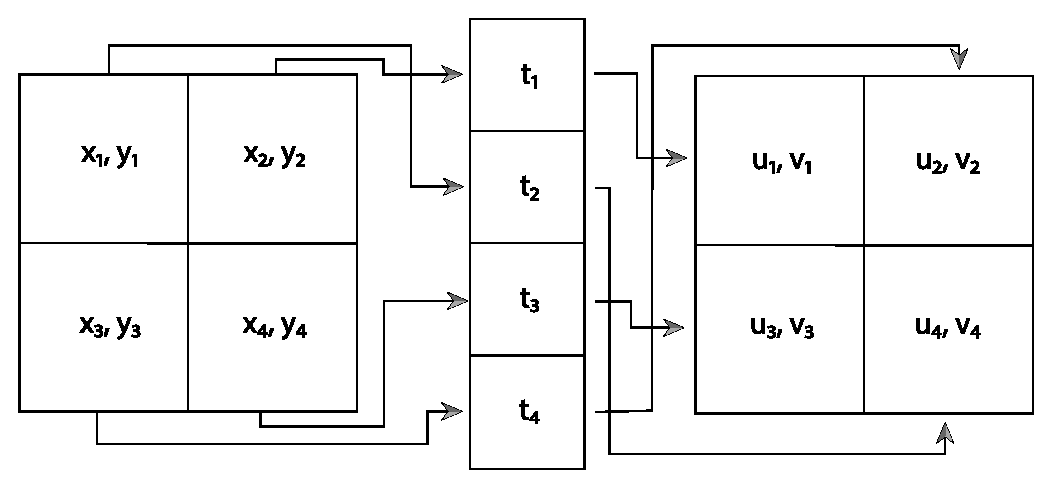
\includegraphics[width=0.8\linewidth]{chap07/Samplepadding.eps}
    \caption{我们可以生成良好的样本模式并获得分层的好处而不要求
        同时对所有采样维度分层。这里,我们已把$(x,y)$图像位置、
        时间$t$以及$(u,v)$透镜位置分为独立的层,每个都有四个区域。
        每个都是独立采样的,然后每个图像样本都随机关联一个时间样本
        和一个透镜样本。我们保留了在每个单独维度上分层的好处而不用指数级地增加样本总量。}
    \label{fig:7.16}
\end{figure}

\reffig{7.17}展示了在渲染景深时使用分层的透镜样本和
使用不分层的随机样本相比图像质量的提升。
\begin{figure}[htbp]
    \subfloat[参考]{
\includegraphics[width=0.49\linewidth]{chap07/dof-ref.png}\label{fig:7.17.1}}\,
    \subfloat[随机采样]{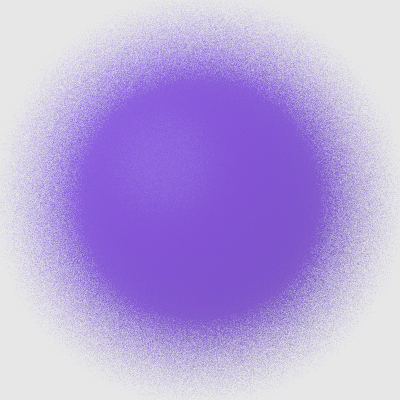
\includegraphics[width=0.49\linewidth]{chap07/dof-random.png}\label{fig:7.17.2}}\\
    \subfloat[分层采样]{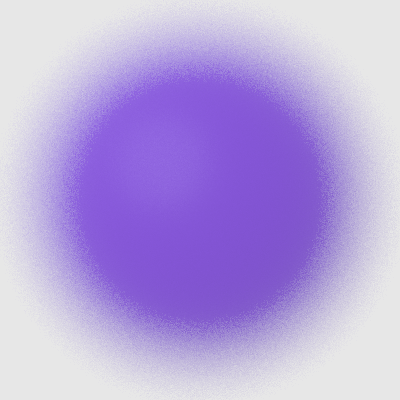
\includegraphics[width=0.49\linewidth]{chap07/dof-stratified.png}\label{fig:7.17.3}}
    \caption{渲染有景深的紫色球体时采样模式的影响。
        (a)模糊球体的高质量参考图像。(b)在每个像素中随机采样而无分层所生成的图像。
        (c)用同样数量的样本生成的图像,但用的是\refvar{StratifiedSampler}{},
        它分层了图像样本以及对该图更重要的透镜样本。对于该情形分层法做出了很大改善。}
    \label{fig:7.17}
\end{figure}

\reffig{7.18}展示比较了几种采样模式。
第一种是完全随机的模式:我们生成大量样本而完全不使用分层。
其结果很差;一些区域只有几个样本而另一些区域有好几团样本。
第二种是均匀分层模式。最后,均匀模式被扰动,
随机偏移量被加到每个样本的位置上,但仍将其保留在格子中。
这给出了比纯随机模式更好的整体分布而又保留了分层的好处,
尽管仍有一些样本团以及欠采样的区域。
\begin{figure}[htbp]
    \subfloat[]{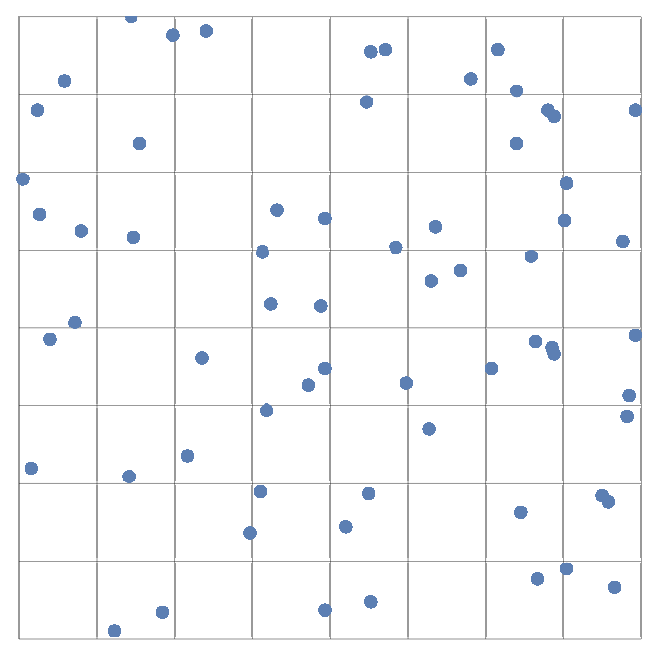
\includegraphics[width=0.49\linewidth]{chap07/random-point-samples.eps}\label{fig:7.18.1}}\,
    \subfloat[]{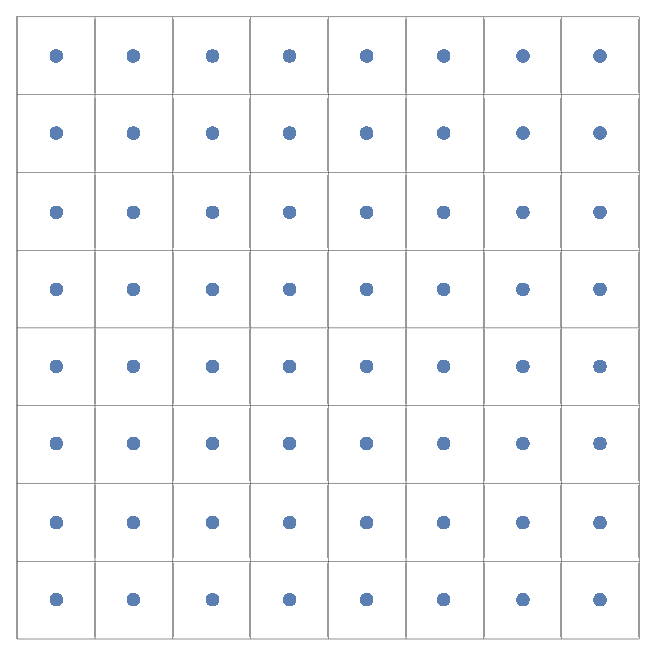
\includegraphics[width=0.49\linewidth]{chap07/uniform-point-samples.eps}\label{fig:7.18.2}}\\
    \subfloat[]{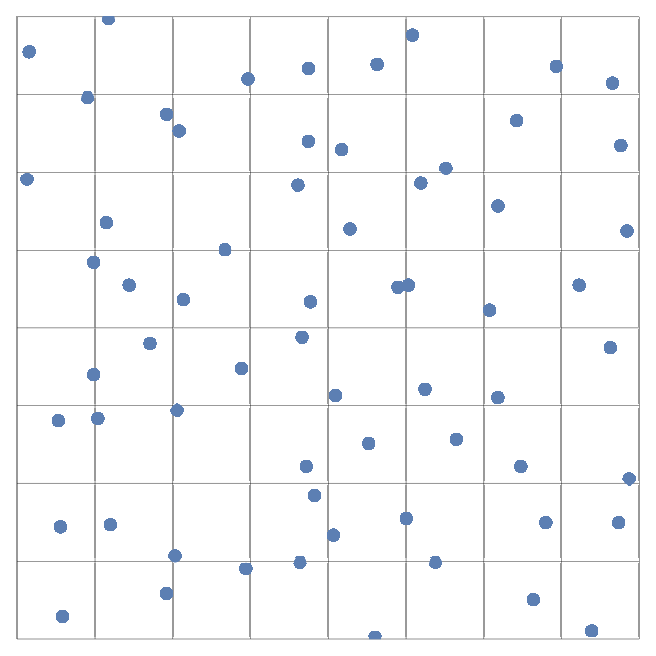
\includegraphics[width=0.49\linewidth]{chap07/jittered-point-samples.eps}\label{fig:7.18.3}}
    \caption{三种2D采样模式。(a)随机模式是无效模式,许多样本团让大片图像没有好好采样。
        (b)均匀分层模式的分布更好但会加剧混叠伪影。
        (c)分层扰动模式将来自均匀模式的混叠转化为高频噪声而仍保留了分层的好处。}
    \label{fig:7.18}
\end{figure}

\reffig{7.19}展示了用\refvar{StratifiedSampler}{}渲染的图像,
并展示了扰动的样本位置怎样将混叠伪影转化为不那么讨厌的噪声。
\begin{figure}[htbp]
    \centering
    \subfloat[参考]{\includegraphics[width=0.8\linewidth]{chap07/checkerboard-ref.png}\label{fig:7.19.1}}\\
    \subfloat[1个均匀样本]{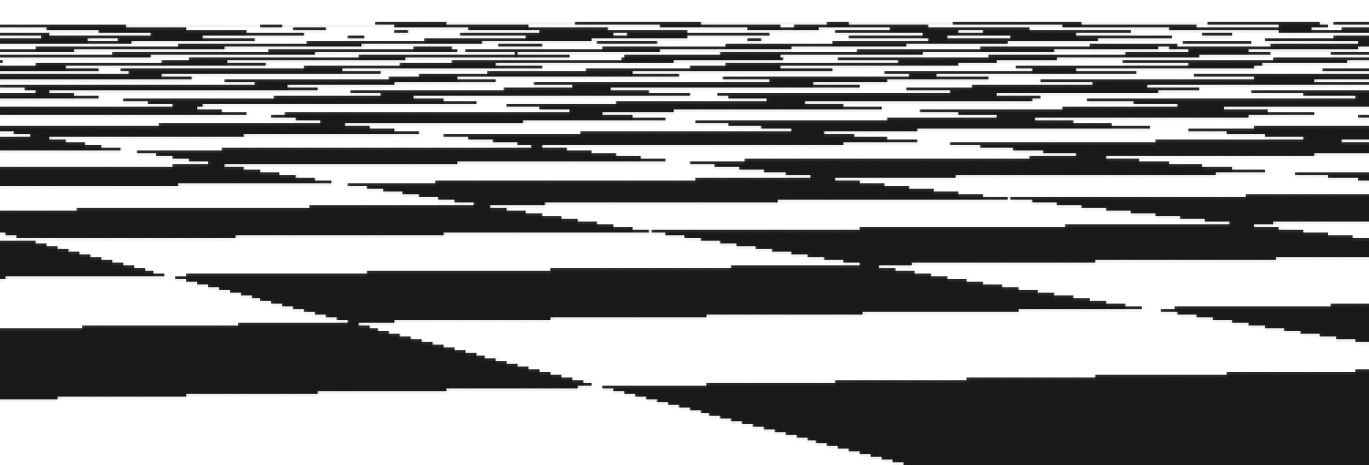
\includegraphics[width=0.8\linewidth]{chap07/checkerboard-unif-1spp.png}\label{fig:7.19.2}}\\
    \subfloat[1个扰动样本]{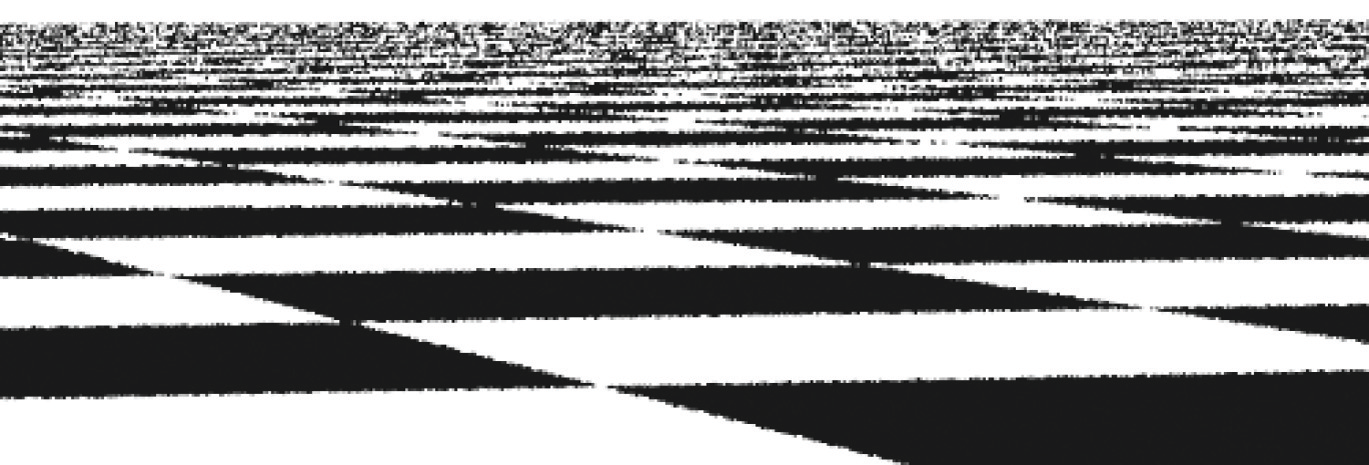
\includegraphics[width=0.8\linewidth]{chap07/checkerboard-jitter-1spp.png}\label{fig:7.19.3}}\\
    \subfloat[4个扰动样本]{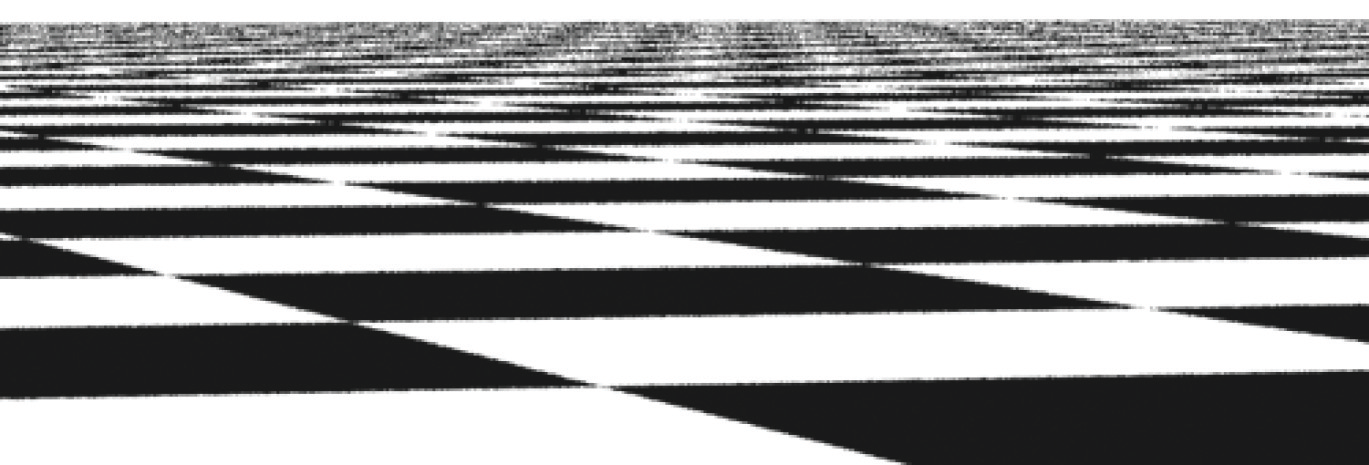
\includegraphics[width=0.8\linewidth]{chap07/checkerboard-jitter-4spp.png}\label{fig:7.19.4}}
    \caption{用棋盘纹理比较图像采样方法。这是幅很难渲染好的图像,
        因为当我们接近地平线时棋盘格关于像素间隔的频率趋于无穷。
        (a)参考图像,每个像素用256个样本渲染,展示了接近理想结果的样子。
        (b)每个像素只用一个样本渲染的图像,没有扰动。注意前景中格子边缘的锯齿伪影。
        还注意棋盘格函数在样本之间经历了许多周期的距离处的伪影;
        如之前介绍过的信号处理理论所料,细节错误地重复表现为低频混叠。
        (c)扰动图像样本的结果,每个像素还是只有一个样本。
        第二幅图像规则的混叠已经被替换为不那么讨厌的噪声伪影。
        (d)每个像素用四个扰动样本的结果仍然不如参考图像,但明显优于之前的结果。}
    \label{fig:7.19}
\end{figure}

\begin{lstlisting}
`\initcode{StratifiedSampler Declarations}{=}`
class `\initvar{StratifiedSampler}{}` : public `\refvar{PixelSampler}{}` {
public:
    `\refcode{StratifiedSampler Public Methods}{}`
private:
    `\refcode{StratifiedSampler Private Data}{}`
};
\end{lstlisting}
\begin{lstlisting}
`\initcode{StratifiedSampler Public Methods}{=}`
`\refvar{StratifiedSampler}{}`(int xPixelSamples, int yPixelSamples,
        bool jitterSamples, int nSampledDimensions)
    : `\refvar{PixelSampler}{}`(xPixelSamples * yPixelSamples, nSampledDimensions),
      `\refvar{xPixelSamples}{}`(xPixelSamples), `\refvar{yPixelSamples}{}`(yPixelSamples),
      `\refvar{jitterSamples}{}`(jitterSamples) { }
\end{lstlisting}
\begin{lstlisting}
`\initcode{StratifiedSampler Private Data}{=}`
const int `\initvar{xPixelSamples}{}`, `\initvar{yPixelSamples}{}`;
const bool `\initvar{jitterSamples}{}`;
\end{lstlisting}

作为\refvar{PixelSampler}{}的子类,
\refvar[StratifiedSampler::StartPixel]{StartPixel}{()}的实现必须按照传给\refvar{PixelSampler}{}
构造函数的维数{\ttfamily nSampledDimensions}一起生成1D和2D样本以及请求的数组样本。
\begin{lstlisting}
`\initcode{StratifiedSampler Method Definitions}{=}`
void `\refvar{StratifiedSampler}{}`::`\initvar[StratifiedSampler::StartPixel]{StartPixel}{}`(const `\refvar{Point2i}{}` &p) {
    `\refcode{Generate single stratified samples for the pixel}{}`
    `\refcode{Generate arrays of stratified samples for the pixel}{}`
    `\refvar{PixelSampler}{}`::StartPixel(p);
}
\end{lstlisting}

生成初始的分层样本后,它们被随机打乱;这是本节开头描述的填充方法。
如果没有进行打乱,则样本维度的值可能以某种方式相关而引发图像中的错误——
例如,用于选择胶片位置的首个2D样本和首个2D透镜样本会总是都在相邻于原点的左下方那层。
\begin{lstlisting}
`\initcode{Generate single stratified samples for the pixel}{=}`
for (size_t i = 0; i < `\refvar{samples1D}{}`.size(); ++i) {
    `\refvar{StratifiedSample1D}{}`(&`\refvar{samples1D}{}`[i][0], `\refvar{xPixelSamples}{}` * `\refvar{yPixelSamples}{}`,
                       `\refvar[PixelSampler::rng]{rng}{}`, `\refvar{jitterSamples}{}`);
    `\refvar{Shuffle}{}`(&`\refvar{samples1D}{}`[i][0], `\refvar{xPixelSamples}{}` * `\refvar{yPixelSamples}{}`, 1, `\refvar[PixelSampler::rng]{rng}{}`);
}
for (size_t i = 0; i < `\refvar{samples2D}{}`.size(); ++i) {
    `\refvar{StratifiedSample2D}{}`(&`\refvar{samples2D}{}`[i][0], `\refvar{xPixelSamples}{}`, `\refvar{yPixelSamples}{}`,
                       `\refvar[PixelSampler::rng]{rng}{}`, `\refvar{jitterSamples}{}`);
    `\refvar{Shuffle}{}`(&`\refvar{samples2D}{}`[i][0], `\refvar{xPixelSamples}{}` * `\refvar{yPixelSamples}{}`, 1, `\refvar[PixelSampler::rng]{rng}{}`);
}
\end{lstlisting}

1D和2D分层采样例程实现为实用函数。
两个都在域中给定层数上循环并在每个里面放置一个样本点。
\begin{lstlisting}
`\initcode{Sampling Function Definitions}{=}\initnext{SamplingFunctionDefinitions}`
void `\initvar{StratifiedSample1D}{}`(`\refvar{Float}{}` *samp, int nSamples, `\refvar{RNG}{}` &rng,
        bool jitter) {
    `\refvar{Float}{}` invNSamples = (`\refvar{Float}{}`)1 / nSamples;
    for (int i = 0; i < nSamples; ++i) {
        `\refvar{Float}{}` delta = jitter ? rng.`\refvar{UniformFloat}{}`() : 0.5f;
        samp[i] = std::min((i + delta) * invNSamples, `\refvar{OneMinusEpsilon}{}`);
    }
}
\end{lstlisting}

\refvar{StratifiedSample2D}{()}同样生成范围$[0,1)^2$中的样本。
\begin{lstlisting}
`\refcode{Sampling Function Definitions}{+=}\lastnext{SamplingFunctionDefinitions}`
void `\initvar{StratifiedSample2D}{}`(`\refvar{Point2f}{}` *samp, int nx, int ny, `\refvar{RNG}{}` &rng,
        bool jitter) {
    `\refvar{Float}{}` dx = (`\refvar{Float}{}`)1 / nx, dy = (`\refvar{Float}{}`)1 / ny;
    for (int y = 0; y < ny; ++y)
        for (int x = 0; x < nx; ++x) {
            `\refvar{Float}{}` jx = jitter ? rng.`\refvar{UniformFloat}{}`() : 0.5f;
            `\refvar{Float}{}` jy = jitter ? rng.`\refvar{UniformFloat}{}`() : 0.5f;
            samp->x = std::min((x + jx) * dx, `\refvar{OneMinusEpsilon}{}`);
            samp->y = std::min((y + jy) * dy, `\refvar{OneMinusEpsilon}{}`);
            ++samp;
        }
}
\end{lstlisting}

函数\refvar{Shuffle}{()}随机重排含有{\ttfamily count}个样本值的数组,
每个都有{\ttfamily nDimensions}维(换句话说,
尺寸为{\ttfamily nDimensions}的值构成的块被重排)。
\begin{lstlisting}
`\initcode{Sampling Inline Functions}{=}\initnext{SamplingInlineFunctions}`
template <typename T>
void `\initvar{Shuffle}{}`(T *samp, int count, int nDimensions, `\refvar{RNG}{}` &rng) {
    for (int i = 0; i < count; ++i) {
        int other = i + rng.`\refvar{UniformUInt32}{}`(count - i);
        for (int j = 0; j < nDimensions; ++j)
            std::swap(samp[nDimensions * i + j],
                      samp[nDimensions * other + j]);
    }
}
\end{lstlisting}

样本数组给我们出了个难题:例如若一个积分器
为像素中的每个样本请求样本向量中含64个2D样本值的数组,
则采样器有两个不同的目标要达成:
\begin{enumerate}
    \item 希望数组内的样本本身在2D上分布良好(例如通过使用$8\times8$分层网格)。
          这里的分层法会为每个单独的样本向量提升算出的结果的质量。
    \item 最好保证一个图像样本的数组中的每个样本都不要和图像中相邻样本的任何样本值太相似。
          即我们更希望点相对于其邻居能分布良好,使得在单个像素周围区域上就能很好覆盖整个样本空间。
\end{enumerate}

比起尝试同时解决这里的两个问题,\refvar{StratifiedSampler}{}只解决第一个。
本章后面的其他采样器会以更加精巧的技术回顾该问题并在不同程度上同时解决它们。

第二个复杂性来自于调用者可能会为每个图像样本请求任意数量样本的事实,
所以可能不易应用分层法。(例如,我们要怎么生成七个样本的分层2D模式?)
我们只能生成一个$n\times1$或$1\times n$的分层模式,
但这只能给我们在一个维度上分层的好处但不保证其他维度有好的模式。
方法{\ttfamily StratifiedSampler::RoundSize()}可以将请求进位到
下一个平方数,但我们将换用一种称为\keyindex{拉丁超立方采样}{Latin hypercube sampling}{}(LHS)的方法,
它能生成具有相当好分布的任意数量的任意维数样本。

LHS把每个维度轴均匀划分为$n$个区域并沿对角线在$n$个区域中的
每一个内生成一个扰动的样本,如\reffig{7.20}左边所示。
然后这些样本在每个维度上被随机打乱,生成分布良好的模式。
\begin{figure}[htbp]
    \centering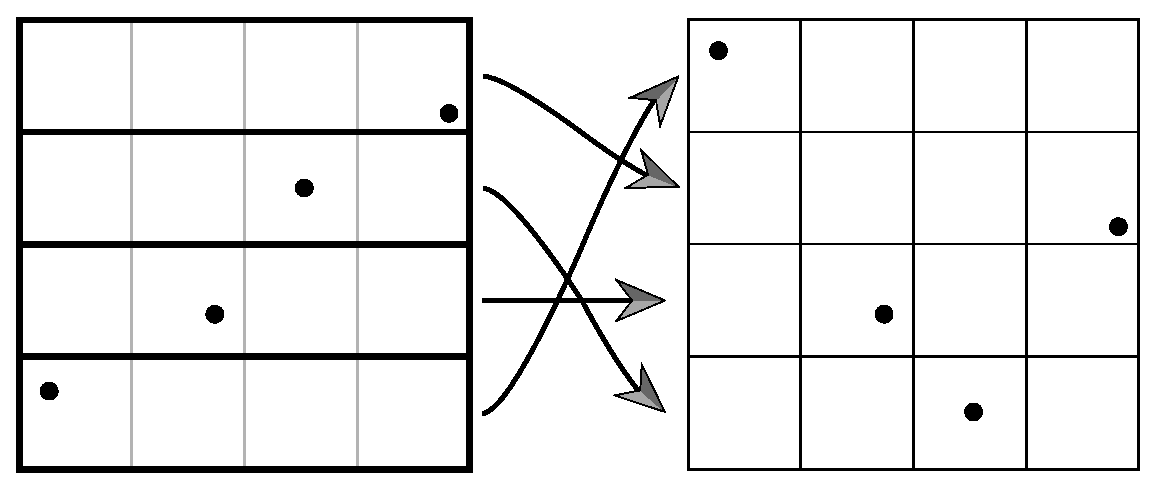
\includegraphics[width=0.8\linewidth]{chap07/LHSshuffle.eps}
    \caption{拉丁超立方采样(有时称为\protect\keyindex{$n$车采样}{$n$-rooks sampling}{})
        选择样本使得网格每行每列只出现单个样本。通过在对角线格子里生成随机样本
        然后随机重排它们的坐标可以做到这点。LHS的一个优点是它能像用分层模式那样
        生成具有良好分布的任意数量的样本,而不仅仅是$m\times n$个样本。}
    \label{fig:7.20}
\end{figure}

LHS的一个优点是当样本投影到样本维度的任意轴时它最小化了样本的聚集。
该性质与分层采样相反,后者2D模式中$n\times n$个样本里的$2n$个可能投影到每个轴上基本相同的点。
\reffig{7.21}展示了对于分层采样模式的这一最坏情况。
\begin{figure}[htbp]
    \centering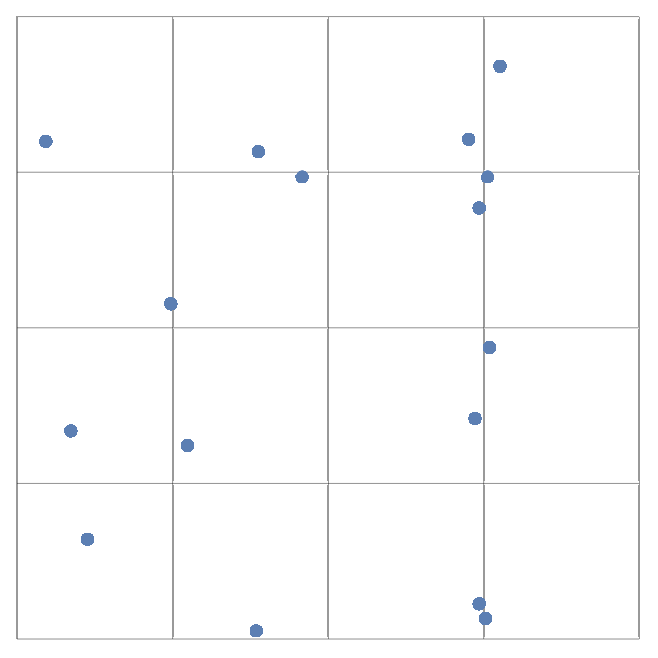
\includegraphics[width=0.4\linewidth]{chap07/stratified-bad-luck.eps}
    \caption{分层采样的一个最坏情况。在$n\times n$的2D模式中,
        多达$2n$个点可能投影到一个轴上基本相同的点。当生成像这样的“倒霉”模式时,
        用其算出的结果质量通常堪忧(这里,8个样本有几乎一样的$x$值)。}
    \label{fig:7.21}
\end{figure}

尽管解决了聚集问题,LHS对于分层采样并不是必要的改进;
很容易构造样本位置基本共线且大面积采样域没有相邻样本的情形
(例如,当原始样本的排列一致时,即让它们都保持原样)。
特别地,随着$n$增加,拉丁超立方模式比起分层模式越来越低效
\footnote{后续章节我们将回顾该问题,讨论同时是分层的且按拉丁超立方模式分布的样本模式。}。

通用的函数\refvar{LatinHypercube}{()}在任意维度生成任意数量的LHS样本。
因此数组{\ttfamily samples}中的元素数量应为{\ttfamily nSamples*nDim}。

\begin{lstlisting}
`\refcode{Sampling Function Definitions}{+=}\lastnext{SamplingFunctionDefinitions}`
void `\initvar{LatinHypercube}{}`(`\refvar{Float}{}` *samples, int nSamples, int nDim, `\refvar{RNG}{}` &rng) {
    `\refcode{Generate LHS samples along diagonal}{}`
    `\refcode{Permute LHS samples in each dimension}{}`
}
\end{lstlisting}
\begin{lstlisting}
`\initcode{Generate LHS samples along diagonal}{=}`
`\refvar{Float}{}` invNSamples = (`\refvar{Float}{}`)1 / nSamples;
for (int i = 0; i < nSamples; ++i)
    for (int j = 0; j < nDim; ++j) {
        `\refvar{Float}{}` sj = (i + (rng.`\refvar{UniformFloat}{}`())) * invNSamples;
        samples[nDim * i + j] = std::min(sj, `\refvar{OneMinusEpsilon}{}`);
    }
\end{lstlisting}

为了进行重排,该函数在样本上循环,每次在一个维度上随机重排样本点。
注意这和之前的\refvar{Shuffle}{()}例程是不一样的重排:
后者例程做一次重排,让每个样本里的全部{\ttfamily nDim}个样本点在一起,
而这里每次做单个维度的{\ttfamily nDim}次单独重排(\reffig{7.22})
\footnote{尽管不需要重排LHS模式的第一维,但这里的实现还是这样做了,
    因为让第一维的元素变为随机顺序意味着LHS模式可以与来自其他源的采样模式
    结合使用而没有其样本点间存在相关性的危险。}。
\begin{figure}[htbp]
    \centering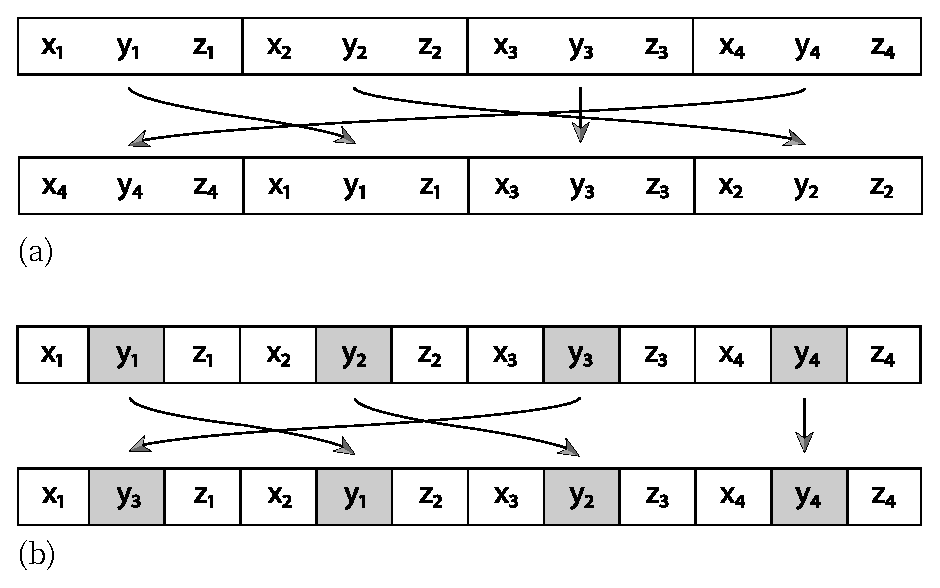
\includegraphics[width=0.8\linewidth]{chap07/Shufflepermutations.eps}
    \caption{(a)\refvar{Shuffle}{()}例程进行的重排移动附近的整块元素。
        (b)拉丁超立方采样的重排独立地排列每个维度的样本。
        这里展示了打乱三维四元素模式的第二维样本。}
    \label{fig:7.22}
\end{figure}

\begin{lstlisting}
`\initcode{Permute LHS samples in each dimension}{=}`
for (int i = 0; i < nDim; ++i) {
    for (int j = 0; j < nSamples; ++j) {
        int other = j + rng.`\refvar{UniformUInt32}{}`(nSamples - j);
        std::swap(samples[nDim * j + i], samples[nDim * other + i]);
    }
}
\end{lstlisting}

有了函数\refvar{LatinHypercube}{()},
我们选择可以编写代码为当前像素计算样本数组了。
1D样本被分层然后随机打乱,而2D样本用拉丁超立方采样生成。
\begin{lstlisting}
`\initcode{Generate arrays of stratified samples for the pixel}{=}`
for (size_t i = 0; i < `\refvar{samples1DArraySizes}{}`.size(); ++i)
    for (int64_t j = 0; j < `\refvar{samplesPerPixel}{}`; ++j) {
        int count = `\refvar{samples1DArraySizes}{}`[i];
        `\refvar{StratifiedSample1D}{}`(&`\refvar{sampleArray1D}{}`[i][j * count], count, `\refvar[PixelSampler::rng]{rng}{}`,
                           `\refvar{jitterSamples}{}`);
        `\refvar{Shuffle}{}`(&`\refvar{sampleArray1D}{}`[i][j * count], count, 1, `\refvar[PixelSampler::rng]{rng}{}`);
    }
for (size_t i = 0; i < `\refvar{samples2DArraySizes}{}`.size(); ++i)
    for (int64_t j = 0; j < `\refvar{samplesPerPixel}{}`; ++j) {
        int count = `\refvar{samples2DArraySizes}{}`[i];
        `\refvar{LatinHypercube}{}`(&`\refvar{sampleArray2D}{}`[i][j * count].x, count, 2, `\refvar[PixelSampler::rng]{rng}{}`);
    }
\end{lstlisting}

我们将用\reffig{7.23}中的场景来阐述一些\refvar{Sampler}{}实现的性质。
\begin{figure}[htbp]
    \centering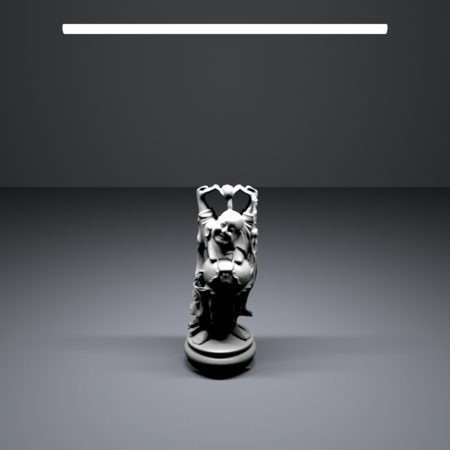
\includegraphics[width=0.6\linewidth]{chap07/area-light-example.png}
    \caption{面光源采样示例场景。}
    \label{fig:7.23}
\end{figure}

\reffig{7.24}展示了对于\refvar{DirectLightingIntegrator}{}来自好样本的提升。
第一幅图像每个像素用1个图像样本算得,每个有16个阴影样本。
第二幅每个像素用16个图像样本,每个有1个阴影样本。
因为\refvar{StratifiedSampler}{}能为第一种情况生成良好的LHS模式,
所以即使在取用的阴影样本总数相同时,其阴影质量也好得多。

\begin{figure}[htbp]
    \centering
    \subfloat[1个图像样本,16个阴影样本]{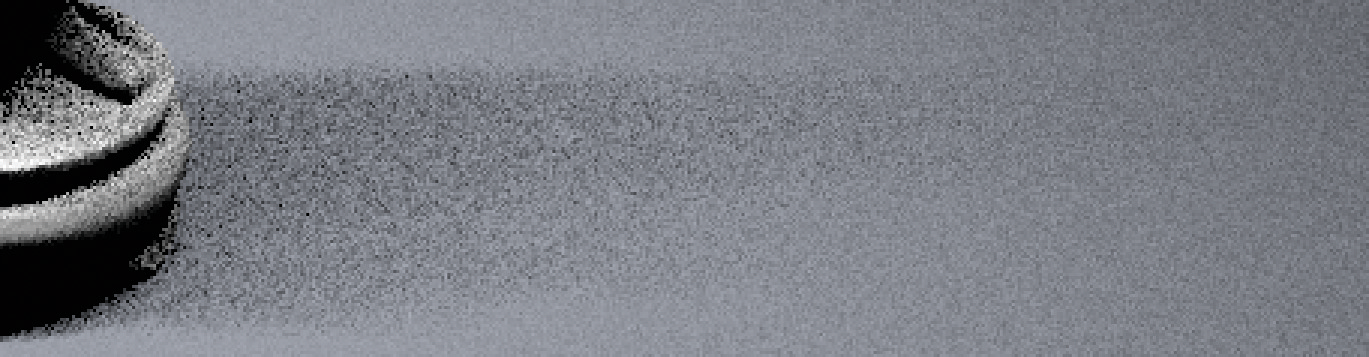
\includegraphics[width=\linewidth]{chap07/shadow-1-16.png}\label{fig:7.24.1}}\\
    \subfloat[16个图像样本,1个阴影样本]{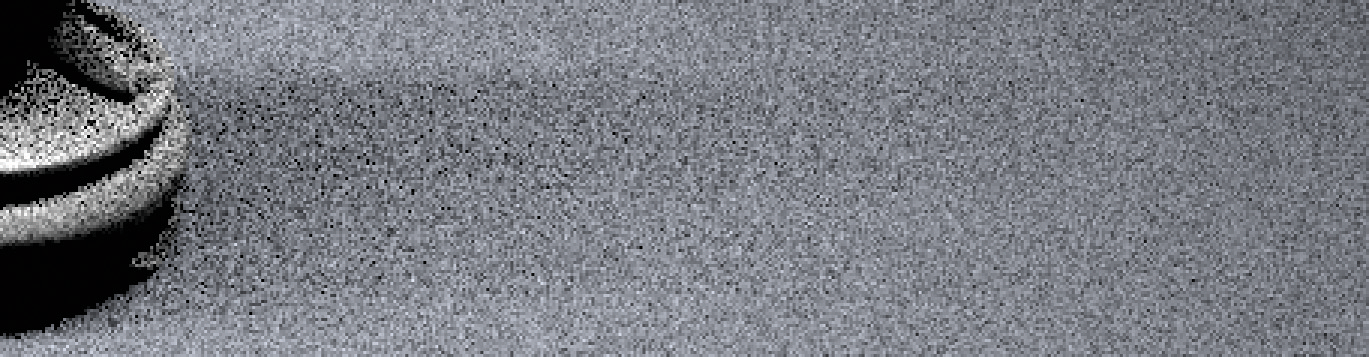
\includegraphics[width=\linewidth]{chap07/shadow-16-1.png}\label{fig:7.24.2}}
    \caption{用来自分层采样器的样本采样面光源。
        (a)展示了每个像素用1个图像样本和16个阴影样本的结果,
        而(b)展示了用16个图像样本且每个只有1个阴影样本的结果。
        两种情况阴影样本的总数是一样的,但因为每个图像样本用16个阴影样本的版本
        可以使用LHS模式,像素区域内所有阴影样本都良好分布,而第二幅图像里
        这里的实现没有办法防止它们分布得很差。差别是惊人的。}
    \label{fig:7.24}
\end{figure}

\section{Halton采样器}\label{sec:Halton采样器}
\begin{remark}
    本节含有高级内容,第一次阅读时可以跳过。
\end{remark}

\refvar{StratifiedSampler}{}的根本目标是生成
分布良好但不均匀的样本点集,使得不存在两个靠得太近的样本点且没有不含样本的过大样本空间区域。
如\reffig{7.18}{}所示,扰动的模式比随机模式做得更好,
不过当相邻层中的样本恰好靠近它们两层的公共边界时其质量可能受影响。

本节介绍\refvar{HaltonSampler}{},它基于直接生成低偏差点集的算法。不像\linebreak
\refvar{StratifiedSampler}{}生成的点集那样,
\refvar{HaltonSampler}{}不仅生成保证不会靠得太近抱团的点,
还生成能同时在样本向量所有维度上都分布良好的点——
而不是像\refvar{StratifiedSampler}{}那样每次只能在一两个维度上做到。

\subsection{Hammersley和Halton序列}\label{sub:Hammersley和Halton序列}
Halton和Hammersley序列是两种紧密相关的低偏差点集。
两者都基于称为\keyindex{倒根}{radical inverse}{}的构造法,
它基于正整数值$a$可以用下式唯一确定的数字序列$d_m(a)\ldots d_2(a)d_1(a)$
表示为$b$进制\sidenote{译者注:这里$b$是大于1的正整数,称为基(数)(base)。}的事实:
\begin{align}
    \label{eq:7.6}
    a=\sum\limits_{i=1}^m{d_i(a)b^{i-1}}\, ,
\end{align}
其中所有数字$d_i(a)$介于0到$b-1$之间。

$b$进制的倒根函数$\varPhi_b$通过将这些数字关于小数点翻转
把非负整数$a$转化为$[0,1)$的小数值:
\begin{align}
    \label{eq:7.7}
    \varPhi_b(a)=0.d_1(a)d_2(a)\ldots d_m(a)\, .
\end{align}
因此,数字$d_i(a)$对倒根的贡献为$\displaystyle\frac{d_i(a)}{b^i}$。

最简单的低偏差序列之一是van der Corput序列
\sidenote{译者注:得名自20世纪荷兰数学家Johannes Gaultherus van der Corput。},
它是由2进制倒根函数给出的1D序列:
\begin{align*}
    x_a=\varPhi_2(a)\, .
\end{align*}

\reftab{7.3}展示了van der Corput序列的前几个值。
注意它怎样递归地将1D直线上的区间对半划分,生成位于每个区间中心的的样本点。
\begin{table}[htbp]
    \centering
    \begin{tabular}{crl}
        \toprule
        $a$      & \textbf{2进制} & $\varPhi_2(a)$      \\
        \midrule
        0        & 0              & $0$                 \\
        1        & 1              & $0.1=\frac{1}{2}$   \\
        2        & 10             & $0.01=\frac{1}{4}$  \\
        3        & 11             & $0.11=\frac{3}{4}$  \\
        4        & 100            & $0.001=\frac{1}{8}$ \\
        5        & 101            & $0.101=\frac{5}{8}$ \\
        $\vdots$ &                &                     \\
        \bottomrule
    \end{tabular}
    \caption{以2进制计算的前几个非负整数的倒根$\varPhi_2(a)$。
        注意$\varPhi_2(a)$的后续值是怎样避开$\varPhi_2(a)$先前的任何值的。
        随着生成该序列越来越多的值,样本必然与之前的样本更加接近,然而仍保证了最小距离足够好。}
    \label{tab:7.3}
\end{table}

该序列的偏差为\sidenote{译者注:这里的大$O$项表明了该偏差的变化趋势。
    事实上它是有界的,相应证明非常复杂,读者可参见\citet{LARCHER2016546}整理的有关结论。}
\begin{align*}
    D^*_N(P)=O\left(\frac{\log N}{N}\right)\, ,
\end{align*}
它与$n$维无限序列取到的最优偏差相匹配,
\begin{align*}
    D^*_N(P)=O\left(\frac{(\log N)^n}{N}\right)\, .
\end{align*}

为了生成$n$维Halton序列,我们使用$b$进制倒根,且模式的每个维度用不同的基。
所用的基必须两两互质,所以自然的选择是使用
前$n$个\keyindex{质数}{prime number}{}$(p_1,\ldots,p_n)$:
\begin{align*}
    x_a=(\varPhi_2(a),\varPhi_3(a),\varPhi_5(a),\ldots,\varPhi_{p_n}(a))\, .
\end{align*}

Halton序列最有用的性质之一是即使不能提前知道所需的样本总量也能用它;
该序列的所有前缀\sidenote{译者注:即序列开头的部分。}都分布良好,
所以向该序列添加额外样本也可保持低偏差(然而对于指数$k_i$,
当样本总数为基的幂之积$\prod(p_i)^{k_i}$时其分布最好)。

$n$维Halton序列的偏差为
\begin{align*}
    D^*_N(x_a)=O\left(\frac{(\log N)^n}{N}\right)\, ,
\end{align*}
它是渐进最优的。

如果固定样本数目$N$,则可以用偏差还低点的Hammersley点集。
Hammersley点集定义为
\begin{align*}
    x_a=\left(\frac{a}{N},\varPhi_{b_1}(a),\varPhi_{b_2}(a),\ldots,\varPhi_{b_n}(a),\right)\, ,
\end{align*}
其中$N$是要取用的样本总数,像之前那样所有基$b_i$都互质。
\reffig{7.25.1}展示了2D Halton序列前216个点的图示。
\reffig{7.25.2}展示了Hammersley序列的前256个点。
\begin{figure}[htbp]
    \centering
    \subfloat[]{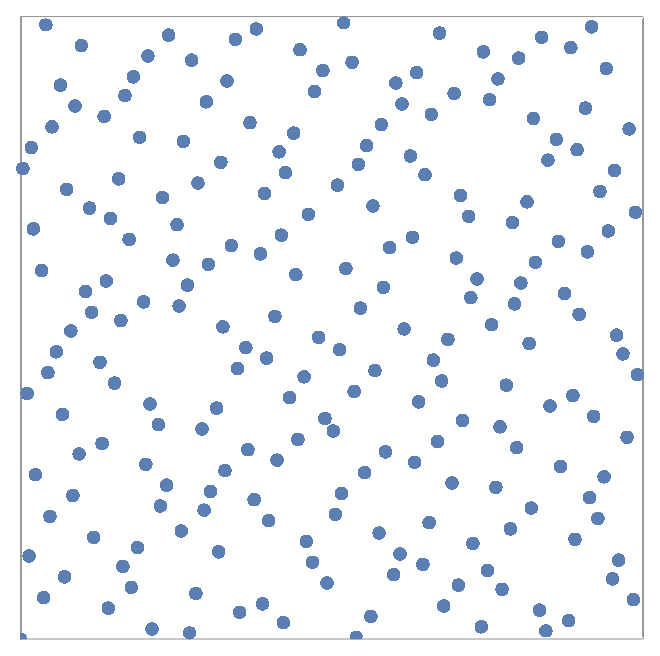
\includegraphics[width=0.49\linewidth]{chap07/halton-points.eps}\label{fig:7.25.1}}\,
    \subfloat[]{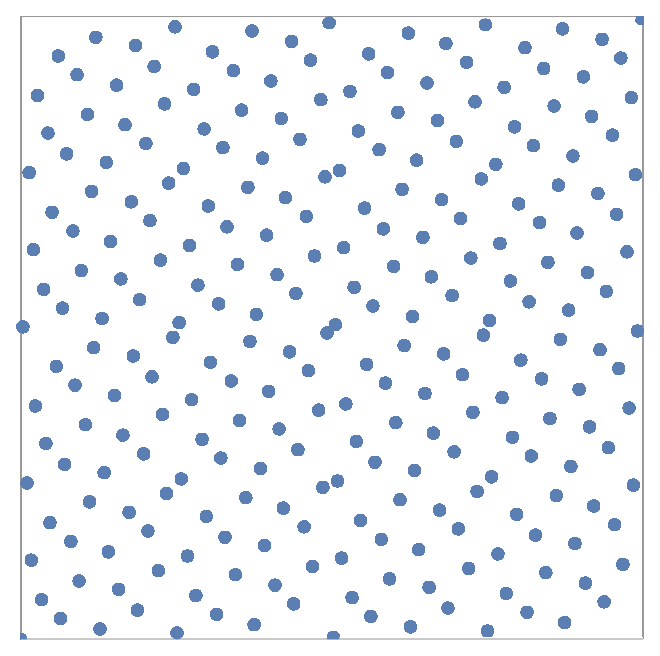
\includegraphics[width=0.49\linewidth]{chap07/hammersley-points.eps}\label{fig:7.25.2}}
    \caption{两种2D低偏差序列前面的点。(a)Halton(216个点),(b)Hammersley(256个点)。}
    \label{fig:7.25}
\end{figure}

函数\refvar{RadicalInverse}{()}用第{\ttfamily baseIndex}个质数
作为基为给定数字{\ttfamily a}计算倒根。
该函数用庞大的{\ttfamily switch}语句实现,其中{\ttfamily baseIndex}被映射到
合适的质数然后由单独的模板函数\refvar{RadicalInverseSpecialized}{()}实际计算该倒根
(稍后将解释使用少见的基于{\ttfamily switch}的结构的原因)。
\begin{lstlisting}
`\initcode{Low Discrepancy Function Definitions}{=}\initnext{LowDiscrepancyFunctionDefinitions}`
`\refvar{Float}{}` `\initvar{RadicalInverse}{}`(int baseIndex, uint64_t a) {
    switch (baseIndex) {
        case 0:
            `\refcode{Compute base-2 radical inverse}{}`
        case 1: return `\refvar{RadicalInverseSpecialized}{}`<3>(a);
        case 2: return `\refvar{RadicalInverseSpecialized}{}`<5>(a);
        case 3: return `\refvar{RadicalInverseSpecialized}{}`<7>(a);
        `\refcode{Remainder of cases for RadicalInverse()}{}`
    }
}
\end{lstlisting}

对于2进制倒根,我们可以利用数字计算机中的数字已经表示为2进制的事实
来更高效地计算倒根。对于一个64位值$a$,按\refeq{7.6}我们有
\begin{align*}
    a=\sum\limits_{i=1}^{64}{d_i(a)2^{i-1}}\, .
\end{align*}
首先考虑翻转$a$数位的结果,仍将其视作整数值,得到
\begin{align*}
    \sum\limits_{i=1}^{64}{d_i(a)2^{64-i}}\, .
\end{align*}
如果我们再用该值除以$2^{64}$,我们有
\begin{align*}
    \sum\limits_{i=1}^{64}{d_i(a)2^{-i}}\, ,
\end{align*}
它就是$\varPhi_2(a)$。因此,2进制倒根可高效地用数位翻转以及2的幂除法算得。

整数量的数位可以用一系列逻辑位运算高效翻转。
翻转32位整数数位的函数\refvar{ReverseBits32}{()}的第一行
交换了该值的低16位和高16位。下一行同时交换其结果的前8位与第二组8位、第三组8位与第四组。
该过程持续到交换相邻数位的最后一行。为了理解该代码,写出各个十六进制常数的二进制值很有帮助。
例如,{\ttfamily 0xff00ff00}的二进制是{\ttfamily 11111111000000001111111100000000};
很容易看到与该值进行按位或屏蔽了第一、三组8位数量。
\begin{lstlisting}
`\initcode{Low Discrepancy Inline Functions}{=}\initnext{LowDiscrepancyInlineFunctions}`
inline uint32_t `\initvar{ReverseBits32}{}`(uint32_t n) {
    n = (n << 16) | (n >> 16);
    n = ((n & 0x00ff00ff) << 8) | ((n & 0xff00ff00) >> 8);
    n = ((n & 0x0f0f0f0f) << 4) | ((n & 0xf0f0f0f0) >> 4);
    n = ((n & 0x33333333) << 2) | ((n & 0xcccccccc) >> 2);
    n = ((n & 0x55555555) << 1) | ((n & 0xaaaaaaaa) >> 1);
    return n;
}
\end{lstlisting}

然后通过单独翻转两个32位分量再互换它们可以翻转64位值的数位。
\begin{lstlisting}
`\refcode{Low Discrepancy Inline Functions}{+=}\lastnext{LowDiscrepancyInlineFunctions}`
inline uint64_t `\initvar{ReverseBits64}{}`(uint64_t n) {
    uint64_t n0 = `\refvar{ReverseBits32}{}`((uint32_t)n);
    uint64_t n1 = `\refvar{ReverseBits32}{}`((uint32_t)(n >> 32));
    return (n0 << 32) | n1;
}
\end{lstlisting}

然后为了计算2进制倒根,我们翻转数位并乘以$\displaystyle\frac{1}{2^{64}}$,
其中十六进制浮点常数{\ttfamily 0x1p-64}用于值$2^{-64}$。
如\refsub{浮点算术}解释的,通过相应的幂2乘法实现幂2除法
会给出以IEEE浮点数表示的相同结果(且浮点数乘法通常比浮点数除法更高效)。
\begin{lstlisting}
`\initcode{Compute base-2 radical inverse}{=}`
return `\refvar{ReverseBits64}{}`(a) * 0x1p-64;
\end{lstlisting}

对于其他基,模板函数\refvar{RadicalInverseSpecialized}{()}计算倒根
是通过计算起始于$d_1$的数字$d_i$并计算一系列$v_i$,
其中$v_1=d_1$,$v_2=bd_1+d_2$,使得
\begin{align*}
    v_n=b^{n-1}d_1+b^{n-2}d_2+\cdots+d_n\, .
\end{align*}
(例如,十进制中它会把值1234转化为4321。)
该值可完全用整数算法求得,不会积累任何舍入误差。

然后倒根的最终值通过转化为浮点并乘以$\displaystyle\frac{1}{b^n}$求得,
其中$n$是该值的位数,由此得到\refeq{7.7}中的值。
该乘法项是在处理数字时在{\ttfamily invBaseN}中构建的。
\begin{lstlisting}
`\initcode{Low Discrepancy Static Functions}{=}\initnext{LowDiscrepancyStaticFunctions}`
template <int base>
static `\refvar{Float}{}` `\initvar{RadicalInverseSpecialized}{}`(uint64_t a) {
    const `\refvar{Float}{}` invBase = (`\refvar{Float}{}`)1 / (`\refvar{Float}{}`)base;
    uint64_t reversedDigits = 0;
    `\refvar{Float}{}` invBaseN = 1;
    while (a) {
        uint64_t next  = a / base;
        uint64_t digit = a - next * base;
        reversedDigits = reversedDigits * base + digit;
        invBaseN *= invBase;
        a = next;
    }
    return std::min(reversedDigits * invBaseN, `\refvar{OneMinusEpsilon}{}`);
}
\end{lstlisting}

一个自然要问的问题是为什么这里要用对基数做参数化的模板函数
(而不是说调用一个把基数作为参数接收的常规函数,避免为每个基生成单独的代码路径)。
动机是在现代CPU上整数除法非常地慢,利用编译时常数除法的方法则能高效得多。

例如,32位值除以3的整数除法可以通过用该值乘以2863311531得到64位中间值
然后将结果右移33位算得;这俩都是非常高效的运算。
(64位值除以3可以用类似方法,但这个神奇常数大得多;
见\citet{10.5555/2462741}\sidenote{译者注:此处引用改为了新版。}了解关于该技术的更多内容。)
因此这里用模板函数允许编译器意识到在{\ttfamily while}循环中计算{\ttfamily next}值的除法时
实际上是除以常数并给它应用该优化的机会。在2015年代笔记本上用了该优化的代码比
基于整数除法指令的实现运行起来快至5.9倍。

另一个优化是我们避免计算翻转数字与倒数基之积的实时总和;
相反,该乘法会一直推迟到结尾直到循环终止。
这里的主要问题是当前处理器的浮点和整数单元是完全互相独立运算的。
在一个紧密循环里的浮点计算中引用一个整数变量会引入管道暂停
\sidenote{译者注:原文pipeline bubble。},
它与转化这些值并从一个单元移动到另一个单元所需的时间相关。

能计算倒根函数的逆会很有用;函数\refvar{InverseRadicalInverse}{()}接收
某进制翻转过的整数数字,即对应于模板函数\refvar{RadicalInverseSpecialized}{()}中
为了转化为$[0,1)$中的浮点值而乘以因子$\displaystyle\frac{1}{b^n}$之前的{\ttfamily reversedDigits}。
注意为了能正确地计算逆,必须知道原始值中的数字总数:
例如倒根算法中在只含整数的部分之后,1234和123400都能转化为4321;
尾部零变为前导零并丢失了。
\begin{lstlisting}
`\refcode{Low Discrepancy Inline Functions}{+=}\lastnext{LowDiscrepancyInlineFunctions}`
template <int base> inline uint64_t
`\initvar{InverseRadicalInverse}{}`(uint64_t inverse, int nDigits) {
    uint64_t index = 0;
    for (int i = 0; i < nDigits; ++i) {
        uint64_t digit = inverse % base;
        inverse /= base;
        index = index * base + digit;
    }
    return index;
}
\end{lstlisting}

Hammersley和Halton序列的缺点是随着基$b$的增加,样本值会展现出惊人的规律模式。
该问题可以用\keyindex{置乱}{scrambled}{}Halton和Hammersley序列解决,
其计算倒根时对数字施加了重排。
\begin{align}
    \label{eq:7.8}
    \varPsi_b(a)=0.p(d_1(a))p(d_2(a))\ldots p(d_m(a))\, ,
\end{align}
其中$p$是数字$(0,1,\ldots,b-1)$的重排。
注意每个数字用的重排是一样的,在给定基$b$下生成所有样本点用的重排也一样。
\reffig{7.26}展示了对Halton序列置乱后的效果。
\begin{figure}[htbp]
    \centering
    \subfloat[]{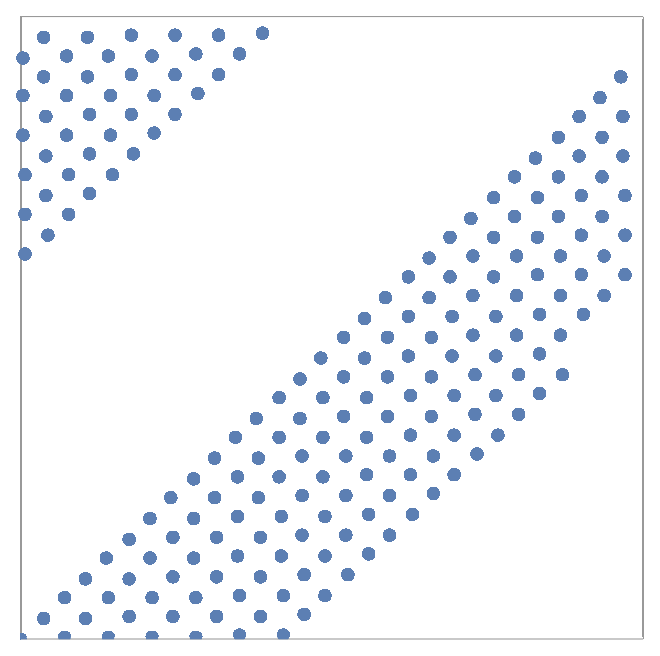
\includegraphics[width=0.45\linewidth]{chap07/halton2931.eps}\label{fig:7.26.1}}\,
    \subfloat[]{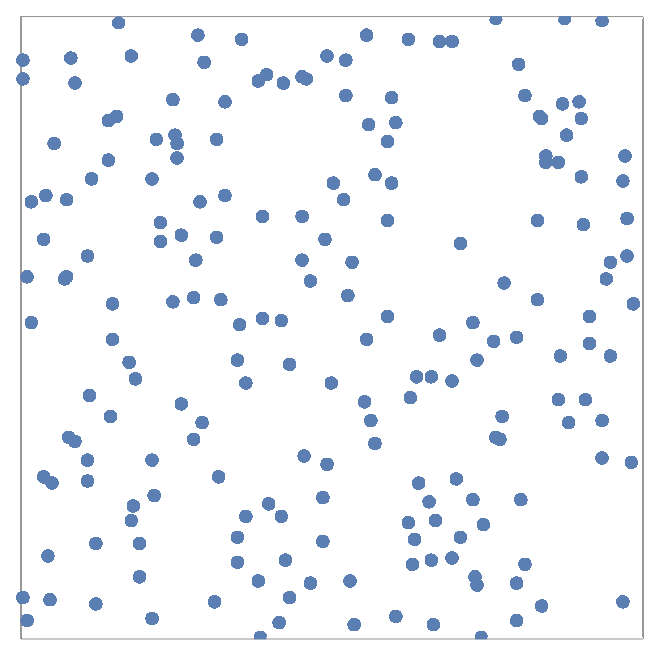
\includegraphics[width=0.45\linewidth]{chap07/halton2931-permuted.eps}\label{fig:7.26.2}}
    \caption{Halton样本值是否有置乱的图示。(a)在样本向量的高维中,
        样本值的投影开始表现出规律结构。这里展示了来自维度$(\varPhi_{29}(a),\varPhi_{31}(a))$的点。
        (b)置乱序列即\refeq{7.8}通过随机重排样本索引的数字打破了该结构。}
    \label{fig:7.26}
\end{figure}

尽管专门构造的重排能给出稍微更好的结构,但接下来我们将用随机重排;
见“扩展阅读”一节了解更多细节。

函数\refvar{ComputeRadicalInversePermutations}{()}计算这些随机重排表。
它为所有重排初始化单个连续数组,其前两个值是$b=2$时整数零和一的重排,
接下来三个值是$b=3$时0、1、2的重排,后续质数基以此类推。
在进入下面的{\ttfamily for}循环时,{\ttfamily p}指向重排数组的起点来为当前的质数基做初始化。
\begin{lstlisting}
`\refcode{Low Discrepancy Function Definitions}{+=}\lastnext{LowDiscrepancyFunctionDefinitions}`
std::vector<uint16_t> `\initvar{ComputeRadicalInversePermutations}{}`(`\refvar{RNG}{}` &rng) {
    std::vector<uint16_t> perms;
    `\refcode{Allocate space in perms for radical inverse permutations}{}`
    uint16_t *p = &perms[0];
    for (int i = 0; i < `\refvar{PrimeTableSize}{}`; ++i) {
        `\refcode{Generate random permutation for ith prime base}{}`
        p += `\refvar{Primes}{}`[i];
    }
    return perms;
}
\end{lstlisting}

重排数组的总大小由直到预先计算的质数表末尾的质数之和给出。
\begin{lstlisting}
`\initcode{Allocate space in perms for radical inverse permutations}{=}`
int permArraySize = 0;
for (int i = 0; i < `\refvar{PrimeTableSize}{}`; ++i)
    permArraySize += `\refvar{Primes}{}`[i];
perms.resize(permArraySize);
\end{lstlisting}
\begin{lstlisting}
`\initcode{Low Discrepancy Declarations}{=}\initnext{LowDiscrepancyDeclarations}`
static constexpr int `\initvar{PrimeTableSize}{}` = 1000;
extern const int `\initvar{Primes}{}`[`\refvar{PrimeTableSize}{}`];
\end{lstlisting}
\begin{lstlisting}
`\initcode{Low Discrepancy Data Definitions}{=}\initnext{LowDiscrepancyDataDefinitions}`
const int `\refvar{Primes}{}`[`\refvar{PrimeTableSize}{}`] = {
    2, 3, 5, 7, 11,
    `\refcode{Subsequent prime numbers}{}`
};
\end{lstlisting}

生成每次重排很简单:我们只需初始化{\ttfamily p}使之指向
对应当前质数长度的同一重排然后随机打乱它的值。
\begin{lstlisting}
`\initcode{Generate random permutation for ith prime base}{=}`
for (int j = 0; j < `\refvar{Primes}{}`[i]; ++j)
    p[j] = j;
`\refvar{Shuffle}{}`(p, `\refvar{Primes}{}`[i], 1, rng);
\end{lstlisting}

函数\refvar{ScrambledRadicalInverse}{()}本质上和\refvar{RadicalInverse}{()}一样,
除了它是通过重排表为给定基数放入每个数字的。
见\refvar{RadicalInverse}{()}之后的习题\ref{sub:7.11.3}了解关于2进制情况下的更高效实现的讨论。
\begin{lstlisting}
`\refcode{Low Discrepancy Function Definitions}{+=}\lastcode{LowDiscrepancyFunctionDefinitions}`
`\refvar{Float}{}` `\initvar{ScrambledRadicalInverse}{}`(int baseIndex, uint64_t a,
        const uint16_t *perm) {
    switch (baseIndex) {
        case 0: return `\refvar{ScrambledRadicalInverseSpecialized}{}`<2>(perm, a);
        case 1: return `\refvar{ScrambledRadicalInverseSpecialized}{}`<3>(perm, a);
        case 2: return `\refvar{ScrambledRadicalInverseSpecialized}{}`<5>(perm, a);
        case 3: return `\refvar{ScrambledRadicalInverseSpecialized}{}`<7>(perm, a);
        `\refcode{Remainder of cases for ScrambledRadicalInverse()}{}`
    }
}
\end{lstlisting}

下面的实现也考虑了当{\ttfamily perm}将数字0映射为非零值时可能出现的特殊情况。
该情况下,一旦{\ttfamily a}到达0迭代就提前停止,
错误地漏掉了值{\ttfamily perm[0]}构成的无限长后继。
幸运的是,这是一个有简单解析解的几何级数,最后一行加上了其值
\sidenote{译者注:以$b=4$、{\ttfamily perm}数组为$[3,2,1,0]$、$a=9$时为例:
$a$以四进制表示为$21$,翻转得$12$,变为四进制浮点数为$0.12$,准确点说是$0.120000\ldots$。
按照重排表{\ttfamily perm}替换数字后应为$0.213333\ldots$。
但代码只处理到前两位即0.21,故应手动加上后面的$0.003333\ldots$。
一般地,应补充的$b$进制数字为$0.\underbrace{0\ldots0}_{m\text{个}0}p(0)p(0)p(0)\ldots$,
其中$m$为$a$的$b$进制位数,依据等比数列求和公式可得
其值是$\displaystyle\frac{b^{-1}p(0)}{1-b^{-1}}b^{-m}$。}。
\begin{lstlisting}
`\refcode{Low Discrepancy Static Functions}{+=}\lastcode{LowDiscrepancyStaticFunctions}`
template <int base>
static `\refvar{Float}{}` `\initvar{ScrambledRadicalInverseSpecialized}{}`(const uint16_t *perm,
        uint64_t a) {
    const `\refvar{Float}{}` invBase = (`\refvar{Float}{}`)1 / (`\refvar{Float}{}`)base;
    uint64_t reversedDigits = 0;
    `\refvar{Float}{}` invBaseN = 1;
    while (a) {
        uint64_t next  = a / base;
        uint64_t digit = a - next * base;
        reversedDigits = reversedDigits * base + perm[digit];
        invBaseN *= invBase;
        a = next;
    }
    return std::min(invBaseN * (reversedDigits +
                    invBase * perm[0] / (1 - invBase)), `\refvar{OneMinusEpsilon}{}`);
}
\end{lstlisting}

\subsection{Halton采样器实现}\label{sub:Halton采样器实现}
\refvar{HaltonSampler}{}用Halton序列生成样本向量。
不像\refvar{StratifiedSampler}{}那样,它是完全确定性的;
在其运算中它没有使用伪随机数。然而,如果没有充分采样好图像,
则Halton样本可能导致混叠。\reffig{7.27}比较了用基于Halton的采样器
和用上一节的分层采样器来采样棋盘纹理的结果。
注意前景中以及朝向地平线处沿边缘的令人难受的模式。
\begin{figure}[htbp]
    \centering
    \subfloat[1个扰动样本]{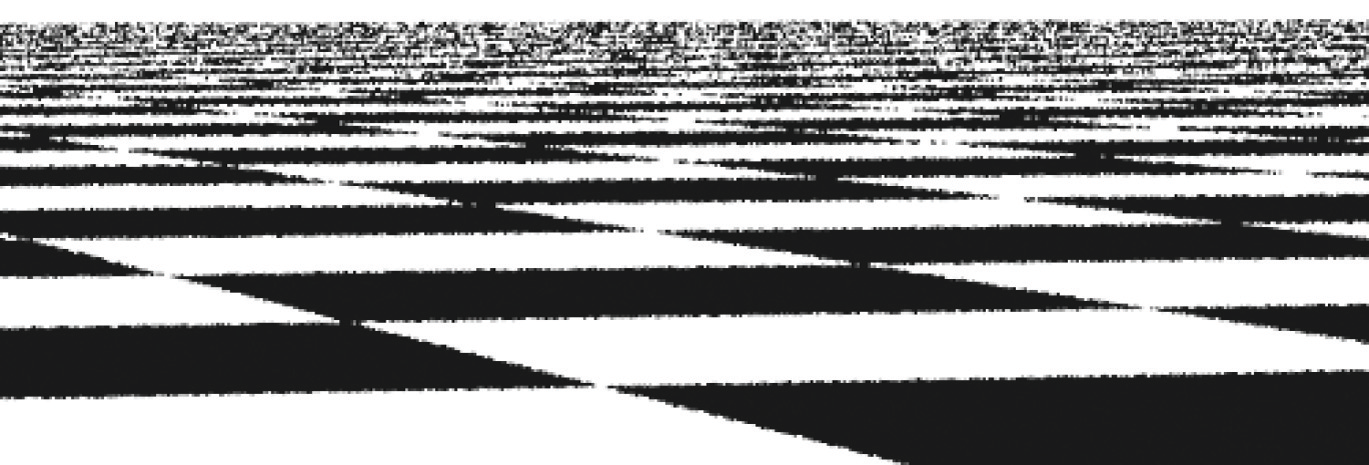
\includegraphics[width=\linewidth]{chap07/checkerboard-jitter-1spp.png}\label{fig:7.27.1}}\\
    \subfloat[1个Halton样本]{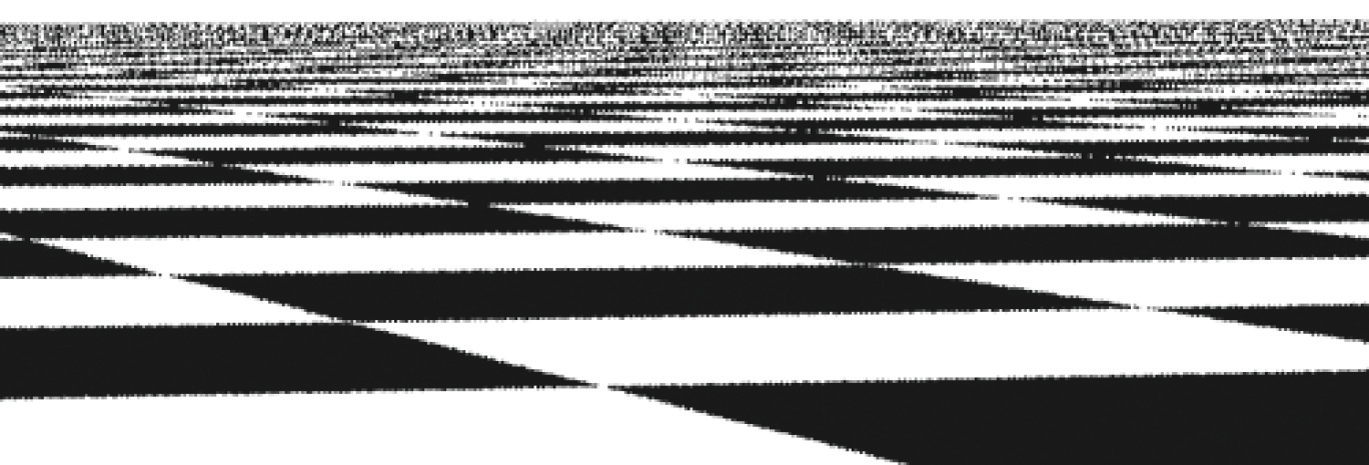
\includegraphics[width=\linewidth]{chap07/checkerboard-halton-1spp.png}\label{fig:7.27.2}}
    \caption{在图像平面上比较分层采样器和基于Halton点的低偏差采样器。
        (a)每个像素只有单个样本的扰动分层采样器与(b)每个像素只有单个样本的\refvar{HaltonSampler}{}采样器。
        注意尽管Halton模式比分层模式更能复现朝向地平线处的棋盘模式,
        但在低偏差模式中仍有干扰视觉注意力的规律性错误结构;
        它没有像扰动法那样把混叠转化为不那么讨厌的噪声。}
    \label{fig:7.27}
\end{figure}

\begin{lstlisting}
`\initcode{HaltonSampler Declarations}{=}`
class `\initvar{HaltonSampler}{}` : public `\refvar{GlobalSampler}{}` {
public:
    `\refcode{HaltonSampler Public Methods}{}`
private:
    `\refcode{HaltonSampler Private Data}{}`
    `\refcode{HaltonSampler Private Methods}{}`
};
\end{lstlisting}
\begin{lstlisting}
`\initcode{HaltonSampler Method Definitions}{=}\initnext{HaltonSamplerMethodDefinitions}`
`\refvar{HaltonSampler}{}`::`\refvar{HaltonSampler}{}`(int samplesPerPixel,
        const `\refvar{Bounds2i}{}` &sampleBounds)
    : `\refvar{GlobalSampler}{}`(samplesPerPixel) {
    `\refcode{Generate random digit permutations for Halton sampler}{}`
    `\refcode{Find radical inverse base scales and exponents that cover sampling area}{}`
    `\refcode{Compute stride in samples for visiting each pixel area}{}`
    `\refcode{Compute multiplicative inverses for baseScales}{}`
}
\end{lstlisting}
\begin{lstlisting}
`\initcode{HaltonSampler Public Methods}{=}`
`\refvar{HaltonSampler}{}`(int nsamp, const `\refvar{Bounds2i}{}` &sampleBounds);
int64_t `\refvar[HaltonSampler::GetIndexForSample]{GetIndexForSample}{}`(int64_t sampleNum) const;
`\refvar{Float}{}` `\refvar[HaltonSampler::SampleDimension]{SampleDimension}{}`(int64_t index, int dimension) const;
std::unique_ptr<`\refvar{Sampler}{}`> `\refvar{Clone}{}`(int seed);
\end{lstlisting}
\begin{lstlisting}
`\initcode{Compute multiplicative inverses for baseScales}{=}`
`\refvar{multInverse}{}`[0] = `\refvar{multiplicativeInverse}{}`(`\refvar{baseScales}{}`[1], `\refvar{baseScales}{}`[0]);
`\refvar{multInverse}{}`[1] = `\refvar{multiplicativeInverse}{}`(`\refvar{baseScales}{}`[0], `\refvar{baseScales}{}`[1]);
\end{lstlisting}

置乱倒根的重排表在所有\refvar{HaltonSampler}{}实例间
共享并在构造函数首次运行时算出。对pbrt的需求而言,该方法很好:
当前实现只是为不同图块使用不同采样器实例,而那时我们想总是使用相同的重排。
对于其他用途,对何时使用不同的重排有更强的控制是值得的。
\begin{lstlisting}
`\initcode{Generate random digit permutations for Halton sampler}{=}`
if (`\refvar{radicalInversePermutations}{}`.size() == 0) {
    `\refvar{RNG}{}` rng;
    `\refvar{radicalInversePermutations}{}` = `\refvar{ComputeRadicalInversePermutations}{}`(rng);
}
\end{lstlisting}
\begin{lstlisting}
`\initcode{HaltonSampler Private Data}{=}\initnext{HaltonSamplerPrivateData}`
static std::vector<uint16_t> `\initvar{radicalInversePermutations}{}`;
\end{lstlisting}

实用方法\refvar{PermutationForDimension}{()}为给定
维度返回指向重排数组起点的指针。
\begin{lstlisting}
`\initcode{HaltonSampler Private Methods}{=}`
const uint16_t *`\initvar{PermutationForDimension}{}`(int dim) const {
    if (dim >= `\refvar{PrimeTableSize}{}`)
        `\refvar{Severe}{}`("HaltonSampler can only sample %d dimensions.",
               `\refvar{PrimeTableSize}{}`);
    return &`\refvar{radicalInversePermutations}{}`[`\refvar{PrimeSums}{}`[dim]];
}
\end{lstlisting}

为了能为给定维度快速找到偏移量,拥有每个质数之前的所有质数之和是很有帮助的。
\begin{lstlisting}
`\refcode{Low Discrepancy Data Definitions}{+=}\lastcode{LowDiscrepancyDataDefinitions}`
const int `\initvar{PrimeSums}{}`[`\refvar{PrimeTableSize}{}`] = {
    0, 2, 5, 10, 17, 
    `\refcode{Subsequent prime sums}{}`
};
\end{lstlisting}

为了把来自$[0,1)^2$的样本前两维映射为像素坐标,
\refvar{HaltonSampler}{}在每个维度上求得比图像分辨率
和\refvar{kMaxResolution}{}中较小者更大的最小缩放因子$(2^j,3^k)$
(我们稍后将看到这一专门选出的缩放值是怎样让看出一个样本在哪个像素里变简单的)。
缩放之后,任何图像范围之外的样本都被简单忽略掉。

对于分辨率在一或两维上大于\refvar{kMaxResolution}{}的图像,
则在全图上重复一块Halton点。该分辨率限制帮助在算得的样本值中保持足够的浮点精度。
\begin{lstlisting}
`\initcode{Find radical inverse base scales and exponents that cover sampling area}{=}`
`\refvar{Vector2i}{}` res = sampleBounds.`\refvar{pMax}{}` - sampleBounds.`\refvar{pMin}{}`;
for (int i = 0; i < 2; ++i) {
    int base = (i == 0) ? 2 : 3;
    int scale = 1, exp = 0;
    while (scale < std::min(res[i], `\refvar{kMaxResolution}{}`)) {
        scale *= base;
        ++exp;
    }
    `\refvar{baseScales}{}`[i] = scale;
    `\refvar{baseExponents}{}`[i] = exp;
}
\end{lstlisting}

对于每个维度,\refvar{baseScales}{}存有缩放因子$2^j$或$3^k$,
且\refvar{baseExponents}{}存有指数$j$和$k$。
\begin{lstlisting}
`\refcode{HaltonSampler Private Data}{+=}\lastnext{HaltonSamplerPrivateData}`
`\refvar{Point2i}{}` `\initvar{baseScales}{}`, `\initvar{baseExponents}{}`;
\end{lstlisting}
\begin{lstlisting}
`\initcode{HaltonSampler Local Constants}{=}`
static constexpr int `\initvar{kMaxResolution}{}` = 128;
\end{lstlisting}

为了明白为什么\refvar{HaltonSampler}{}使用该方案来
将样本映射到像素坐标,考虑用$b$进制倒根因子$b^n$来缩放算出的值的影响。
如果$a$的数字表示为$b$进制的$d_i(a)$,则回想倒根为$b$进制的值$0.d_1(a)d_2(a)\ldots$。
例如,如果我们用$b^2$乘以该值,则我们有$d_1(a)d_2(a).d_3(a)\ldots$;
前两个数字被移到小数点左边,该值的小数部分从$d_3(a)$开始。

用$b^n$缩放的该运算构建了能够确定哪个样本索引位于哪个像素中的核心。
考虑上面例子中的前两个数字,我们可以看到缩放后的值的整数部分在0到$b^2-1$的范围内,
且随着$a$增加,在该范围内每过$b^2$个值,其$b$进制的最后两个数字就在某特定值上取得一次。

给定值$x$,$0\le x\le b^2-1$,我们可以求得首个整数部分为$x$的值$a$。
根据定义,$b$进制的$x$数字为$d_2(x)d_1(x)$。
因此,如果$d_1(a)=d_2(x)$且$d_2(a)=d_1(x)$,
则$a$的倒根被缩放后的值会有等于$x$的整数部分。

因为\refvar{HaltonSampler}{}中为像素样本用的基$b=2$和$b=3$是互质的,
所以它满足如果样本值由某个$(2^j,3^k)$缩放,则在
范围$(0,0)\rightarrow(2^j-1,3^k-1)$内的任意特定像素
每过$2^j3^k$个样本就会访问一次。该乘积存于\refvar{sampleStride}{}中。
\begin{lstlisting}
`\initcode{Compute stride in samples for visiting each pixel area}{=}`
`\refvar{sampleStride}{}` = `\refvar{baseScales}{}`[0] * `\refvar{baseScales}{}`[1];
\end{lstlisting}
\begin{lstlisting}
`\refcode{HaltonSampler Private Data}{+=}\lastnext{HaltonSamplerPrivateData}`
int `\initvar{sampleStride}{}`;
\end{lstlisting}
\begin{lstlisting}
`\refcode{HaltonSampler Private Data}{+=}\lastnext{HaltonSamplerPrivateData}`
int `\initvar{multInverse}{}`[2];
\end{lstlisting}

位于\refvar{currentPixel}{}内的首个Halton样本的样本索引存于\refvar{offsetForCurrentPixel}{}
中。在为当前像素中的首个样本算出该偏移量后,该像素中的后续样本
可在Halton序列中增量为\refvar{sampleStride}{}的样本处找到
\sidenote{译者注:指索引每增加\refvar{sampleStride}{}就出现一次该像素的样本。}。
\begin{lstlisting}
`\refcode{HaltonSampler Method Definitions}{+=}\lastnext{HaltonSamplerMethodDefinitions}`
int64_t `\refvar{HaltonSampler}{}`::`\initvar[HaltonSampler::GetIndexForSample]{\refvar{GetIndexForSample}{}}{}`(int64_t sampleNum) const {
    if (`\refvar{currentPixel}{}` != `\refvar{pixelForOffset}{}`) {
        `\refcode{Compute Halton sample offset for currentPixel}{}`
        `\refvar{pixelForOffset}{}` = `\refvar{currentPixel}{}`;
    }
    return `\refvar{offsetForCurrentPixel}{}` + sampleNum * `\refvar{sampleStride}{}`;
}
\end{lstlisting}
\begin{lstlisting}
`\refcode{HaltonSampler Private Data}{+=}\lastcode{HaltonSamplerPrivateData}`
mutable `\refvar{Point2i}{}` `\initvar{pixelForOffset}{}` = `\refvar{Point2i}{}`(std::numeric_limits<int>::max(),
                                         std::numeric_limits<int>::max());
mutable int64_t `\initvar{offsetForCurrentPixel}{}`;
\end{lstlisting}

在给定像素$(x,y)$内计算首个已被$(2^j,3^k)$缩放的样本索引
包括计算$x$的2进制最后$j$个数字的逆倒根,我们将其记作$x_r$,
以及$y$的3进制最后$k$个数字的逆倒根$y_r$。这为我们给出了方程组
\begin{align*}
    x_r & \equiv(i \mod 2^j)\, , \\
    y_r & \equiv(i \mod 3^k)\, ,
\end{align*}
其中满足该方程组的索引$i$就是位于给定像素内缩放后的样本索引。
本书中我们没有包含这里解出$i$的代码{\refcode{Compute Halton sample offset for currentPixel}{}}
\sidenote{译者注:我补充回来了。};见Gr\"{u}nschlo\ss{}和Keller \parencite*{10.1007/978-3-642-04107-5_25}
了解用于求解$i$的该算法的细节\sidenote{译者注:参考文献列表中作者名字
    中的德文字母“\ss{}”错误显示为“SS”,目前无法解决,请读者见谅。
    同时欢迎提供解决办法!此外,原文引用的文献将年份误写为2012,已修正。}。
\begin{lstlisting}
`\initcode{Compute Halton sample offset for currentPixel}{=}`
`\refvar{offsetForCurrentPixel}{}` = 0;
if (`\refvar{sampleStride}{}` > 1) {
    `\refvar{Point2i}{}` pm(`\refvar{Mod}{}`(`\refvar{currentPixel}{}`[0], `\refvar{kMaxResolution}{}`),
               `\refvar{Mod}{}`(`\refvar{currentPixel}{}`[1], `\refvar{kMaxResolution}{}`));
    for (int i = 0; i < 2; ++i) {
        uint64_t dimOffset = (i == 0) ?
            `\refvar{InverseRadicalInverse}{}`<2>(pm[i], `\refvar{baseExponents}{}`[i]) :
            `\refvar{InverseRadicalInverse}{}`<3>(pm[i], `\refvar{baseExponents}{}`[i]);
        `\refvar{offsetForCurrentPixel}{}` += dimOffset * (`\refvar{sampleStride}{}` / `\refvar{baseScales}{}`[i]) * `\refvar{multInverse}{}`[i];
    }
    `\refvar{offsetForCurrentPixel}{}` %= `\refvar{sampleStride}{}`;
}
\end{lstlisting}

样本偏移量的计算不考虑随机数字重排,所以在这里算出的样本值中没有包含它们。
此外,因为前两维中低处的\refvar{baseExponents}{[i]}个数字用于选择采样哪个样本,
所以这些数字必须在为样本向量的前两维计算倒根之前就被丢弃掉,
此后方法\refvar[HaltonSampler::SampleDimension]{SampleDimension}{()}应该返回正被采样的像素内的小数偏移量。
更高维则被直接采样,包含随机重排。
\begin{lstlisting}
`\refcode{HaltonSampler Method Definitions}{+=}\lastcode{HaltonSamplerMethodDefinitions}`
`\refvar{Float}{}` `\refvar{HaltonSampler}{}`::`\initvar[HaltonSampler::SampleDimension]{\refvar{SampleDimension}{}}{}`(int64_t index, int dim) const {
    if (dim == 0)
        return `\refvar{RadicalInverse}{}`(dim, index >> `\refvar{baseExponents}{}`[0]);
    else if (dim == 1)
        return `\refvar{RadicalInverse}{}`(dim, index / `\refvar{baseScales}{}`[1]);
    else
        return `\refvar{ScrambledRadicalInverse}{}`(dim, index,
            `\refvar{PermutationForDimension}{}`(dim));
}
\end{lstlisting}

\section{(0,2)序列采样器}\label{sec:(0,2)序列采样器}
\begin{remark}
    本节含有高级内容,第一次阅读时可以跳过。
\end{remark}

另一个生成高质量样本的方法是利用某些低偏差序列的显著性质
即允许我们满足两个想要的样本性质(其中仅一个用\refvar{StratifiedSampler}{}满足了):
它们为图像样本的一个像素值生成样本向量使得每个像素样本的样本值都彼此间分布良好,
同时该像素中所有像素样本的样本值集合也整体上分布良好。

该序列使用Sobol\footnote{\protect\refsec{Sobol采样器}的\refvar{SobolSampler}{}使用了
    Sobol序列的所有维度。}推导出的低偏差序列的前两维。
该序列是一种特殊类型的低偏差序列,称为$(0,2)$序列。
$(0,2)$序列以非常常规的方式分层。例如,$(0,2)$序列中的前16个样本
满足来自\refsec{分层采样}中分层采样的分层约束,
意味着每个范围为$\displaystyle\left(\frac{1}{4},\frac{1}{4}\right)$的矩形中只存在一个样本。
然而它们还满足拉丁超立方约束,即在每个范围为$\displaystyle\left(\frac{1}{16},1\right)$和
$\displaystyle\left(1,\frac{1}{16}\right)$的矩形中只有一个样本。
此外,在每个范围为$\displaystyle\left(\frac{1}{2},\frac{1}{8}\right)$和
$\displaystyle\left(\frac{1}{8},\frac{1}{2}\right)$的矩形中只有一个样本。

\reffig{7.28}展示了划分域的所有可能,其中$(0,2)$序列前16个样本都满足分层性质。
从该模式中获取的每组含16个样本的后续序列也都满足这些分布性质。
\begin{figure}[htbp]
    \centering
    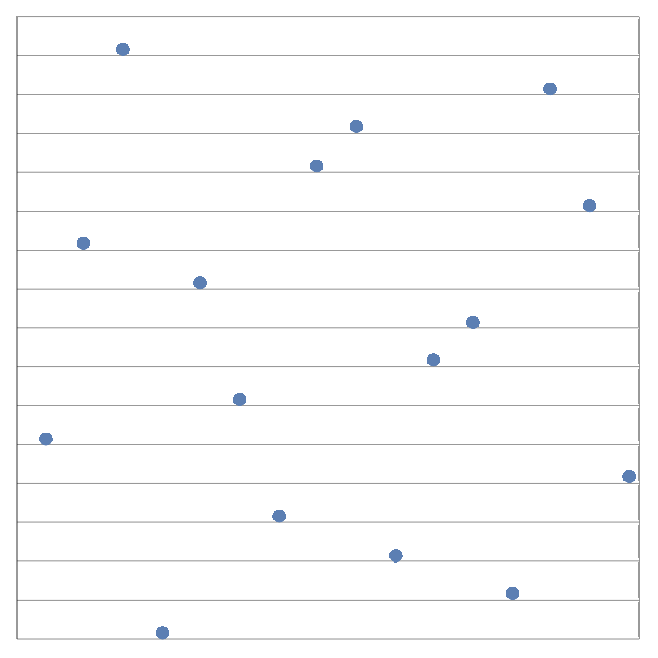
\includegraphics[width=0.49\linewidth]{chap07/elementary1x16.eps}\,
    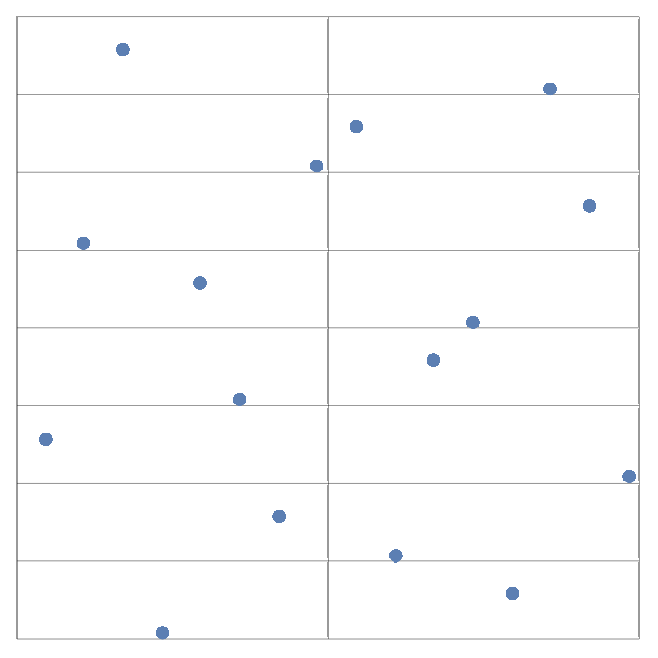
\includegraphics[width=0.49\linewidth]{chap07/elementary2x8.eps}\\
    \includegraphics[width=0.49\linewidth]{chap07/elementary4x4.eps}\,
    \includegraphics[width=0.49\linewidth]{chap07/elementary8x2.eps}\\
    \includegraphics[width=0.49\linewidth]{chap07/elementary16x1.eps}
    \caption{在所有以2为底数的基本区间中都只有单个样本的采样模式。
        它同时满足$4\times4$分层和拉丁超立方约束以及所示的其他两个分层约束。}
    \label{fig:7.28}
\end{figure}

通常任何来自$(0,2)$序列的长为$2^{l_1+l_2}$的序列(其中$l_i$为非负整数)
都满足该一般分层约束。以2为底的两维的\keyindex{基本区间}{elementary interval}{}定义为
\begin{align*}
    E=\left\{\left[\frac{a_1}{2^{l_1}},\frac{a_1+1}{2^{l_1}}\right)\times\left[\frac{a_2}{2^{l_2}},\frac{a_2+1}{2^{l_2}}\right)\right\}\, ,
\end{align*}
其中整数$a_i=0,1,2\ldots,2^{l_i}-1$.
该序列中前$2^{l_1+l_2}$个值中的每一个样本都在相应基本区间中。
此外,后续每$2^{l_1+l_2}$个值构成的集合也满足同样的性质。

现在为了理解怎样把$(0,2)$序列应用于生成2D样本,
考虑有$2\times2$图像样本的像素,每个含$4\times4$个2D样本构成的数组。
依据相应的基本区间集,$(0,2)$序列前$(2\times2)\times(4\times4)=2^6$个值相互之间分布良好。
此外依据其相应的基本区间,前$4\times4=2^4$个样本自己也分布良好,
其后的$2^4$个也是这样,以此类推。因此,我们可以为一个像素的
首个图像样本的$4\times4$数组样本使用前16个$(0,2)$序列样本,
然后下一个图像样本用接下来的16个,以此类推。
结果是分布非常良好的样本点集。

\subsection{用生成矩阵采样}\label{sub:用生成矩阵采样}
比起\refvar{HaltonSampler}{},Sobol序列基于不同的样本点生成机制,
它在各维度上使用了倒根。即使将倒根函数中的整数除法转化为乘法和位移,
高质量高分辨率渲染所需的计算数十亿样本的计算量也会很大。
大部分计算开销来自于在天生是2进制的计算机上执行不以2为底的计算
(考虑代码片\refcode{Compute base-2 radical inverse}{}和模板函数\refvar{RadicalInverseSpecialized}{()}间的差别)。

假设不以2为底的计算有很高开销,自然要尝试开发完全用2进制运算的样本生成算法。
一个这样高效的方法是用\keyindex{生成矩阵}{generator matrix}{},
它允许在相同基中完成所有计算。不像Halton采样器那样在每个维度使用不同基,
它在每个维度使用不同生成矩阵。为每个采样维度精选好矩阵,
就能生成非常好的低偏差分布点。例如,$(0,2)$序列可用两个特定的2进制生成矩阵定义。

为了看看怎样使用生成矩阵,考虑一个$n$位$b$进制数$a$,
其中$a$的第$i$个数字是$d_i(a)$,且我们有个$n\times n$生成矩阵$\bm C$.
则相应样本点$x_a\in[0,1)$定义为
\begin{align}\label{eq:7.9}
    x_a=[b^{-1}\,b^{-2}\, \cdots\,b^{-n}]\left[
        \begin{array}{cccc}
            c_{1,1} & c_{1,2} & \cdots & c_{1,n} \\
            c_{2,1} & \ddots  &        & c_{2,n} \\
            \vdots  &         & \ddots & \vdots  \\
            c_{n,1} & \cdots  & \cdots & c_{n,n}
        \end{array}
        \right]
    \left[
        \begin{array}{c}
            d_1(a) \\
            d_2(a) \\
            \vdots \\
            d_n(a)
        \end{array}
        \right]\, ,
\end{align}
其中的所有运算都在环$\mathsf{Z}_b$中执行(换句话说,所有运算都按模$b$执行)。
当$a$从0变到$b^n-1$时,这一构造给出一共$b^n$个点。
如果该生成矩阵是单位矩阵,则该定义对应于常规的基$b$倒根
(在继续之前,值得你停下来看看\refeq{7.7}与\refeq{7.9}间的联系)。

本节中,我们将只用$b=2$和$n=32$.尽管把$32\times32$矩阵引入样本生成算法
可能看似不是迈向更优性能的一步,但我们最终将看到采样代码可以映射为
以极为高效的方式用少量位运算执行该计算的实现。

迈向高性能的第一步来自我们按2进制处理的事实;
这样$\bm C$的所有元素不是0就是1,
且因此我们可以把矩阵每行或每列表示为一个无符号32位整数。
我们将选择把矩阵的列表示为{\ttfamily uint32\_t};
该抉择得到一个让$d_i$列向量和$\bm C$相乘的非常高效的算法。

现在考虑计算矩阵-向量乘积${\bm C}[d_i(a)]^{\mathrm{T}}$的任务;
利用矩阵-向量乘积的定义,我们有:
\begin{align}\label{eq:7.10}
    \left[
        \begin{array}{cccc}
            c_{1,1} & c_{1,2} & \cdots & c_{1,n} \\
            c_{2,1} & \ddots  &        & c_{2,n} \\
            \vdots  &         & \ddots & \vdots  \\
            c_{n,1} & \cdots  & \cdots & c_{n,n}
        \end{array}
        \right]\left[
        \begin{array}{c}
            d_1(a) \\
            d_2(a) \\
            \vdots \\
            d_n(a)
        \end{array}
        \right]
    =d_1\left[
        \begin{array}{c}
            c_{1,1} \\
            c_{2,1} \\
            \vdots  \\
            c_{n,1}
        \end{array}
        \right]+\cdots+d_n\left[
        \begin{array}{c}
            c_{1,n} \\
            c_{2,n} \\
            \vdots  \\
            c_{n,n}
        \end{array}
        \right]\, .
\end{align}
换句话说,对于$d_i$每个值为1的数字,$\bm C$的对应列应被求和。
该加法反过来可以在$\mathsf{Z}_2$中高效执行:
在该设置下,加法对应于异或运算(考虑两个运算值可能的组合——
0和1——相加$\mod{2}$的结果,并与同样运算值异或后算出的值比较)。
因此,乘法${\bm C}[d_i(a)]^{\mathrm{T}}$只是在$d_i(a)$位为1处
将$\bm C$的第$i$列异或在一起。该计算在函数\refvar{MultiplyGenerator}{()}中实现。
\begin{lstlisting}
`\refcode{Low Discrepancy Inline Functions}{+=}\lastnext{LowDiscrepancyInlineFunctions}`
inline uint32_t `\initvar{MultiplyGenerator}{}`(const uint32_t *C, uint32_t a) {
    uint32_t v = 0;
    for (int i = 0; a != 0; ++i, a >>= 1)
        if (a & 1)
            v ^= C[i];
    return v;
}
\end{lstlisting}

现在回到\refeq{7.9},若我们把积中的列向量
记为$v={\bm C}[d_i(a)]^{\mathrm{T}}$,则考虑向量积
\begin{align}\label{eq:7.11}
    x_a=[2^{-1}\, 2^{-2}\,\cdots\, 2^{-n}]\left[
        \begin{array}{c}
            v_1    \\
            v_2    \\
            \vdots \\
            v_n
        \end{array}
        \right]=\sum\limits_{i=1}^{32}{2^{-i}v_i}\, .
\end{align}
因为$v$的元素存于单个{\ttfamily uint32\_t},其值理解为{\ttfamily uint32\_t}时是
\begin{align*}
    v=v_1+2v_2+\cdots=\sum\limits_{i=1}^{32}{2^{i-1}v_i}\, .
\end{align*}
如果我们翻转{\ttfamily uint32\_t}内的数位顺序,则我们将有值
\begin{align*}
    v'=\sum\limits_{i=1}^{32}{2^{32-i}v_i}\, .
\end{align*}
这是更有用的值:如果我们将该值除以$2^{32}$,则我们得到\refeq{7.11},
即我们要尝试算出的$x_a$.

因此,如果我们取函数\refvar{MultiplyGenerator}{()}的结果,
颠倒返回值的数位顺序(例如用\refvar{ReverseBits32}{()}),
再用该值除以$2^{32}$以计算$[0,1)$中的浮点数,我们就算出了样本值。

为了节约翻转数位的小小开销,我们可以在传入\refvar{MultiplyGenerator}{()}之前
等价地翻转生成矩阵$\bm C$所有列的数位。接下来我们将遵循该约定。

实践中为了让$(0,2)$序列有用,我们还需要能为
每个图像样本生成多个不同的2D样本值集合,
且我们想为每个像素生成不同的样本值。
该问题的一个方法是为每个像素使用从$(0,2)$序列精选的不重叠子序列
\footnote{\refsec{Sobol采样器}的Sobol采样器采用该方法。}。
另一种方法是随机置乱$(0,2)$序列,通过把随机重排应用于原始序列值$b$进制数字
而构建得到新的$(0,2)$序列。

我们将用的置乱方法归功于\citet{10.1111/1467-8659.00706}。
它反复划分与打乱单位方形$[0,1)^2$.
在这两维的每一个中,它都先将该方形对半分再以50\%的概率交换这两半。
然后它再分别对半划分区间$[0,0.5)$和$[0.5,1)$并随机交换其两半。
该过程递归持续直到2进制表示的所有数位都处理完。
仔细设计该过程使其保留点集的低偏差性质;否则$(0,2)$序列的优势会在置乱时流失。
\reffig{7.29}展示了未置乱的$(0,2)$序列及其两个随机置乱的变种。
\begin{figure}[htbp]
    \centering
    \subfloat[]{\includegraphics[width=0.3\linewidth]{chap07/02-a.eps}\label{fig:7.29.1}}\quad
    \subfloat[]{\includegraphics[width=0.3\linewidth]{chap07/02-b.eps}\label{fig:7.29.2}}\quad
    \subfloat[]{\includegraphics[width=0.3\linewidth]{chap07/02-c.eps}\label{fig:7.29.3}}
    \caption{(a)基于低偏差$(0,2)$序列的采样模式以及(b,c)其两个随机置乱的例子。
        若我们在每个像素中用相同的采样模式,则图像中可能出现伪影,
        而低偏差模式的随机置乱是消除它的高效方法,且仍保留所用点集的低偏差性质。}
    \label{fig:7.29}
\end{figure}

函数\refvar{SampleGeneratorMatrix}{()}将这些片段组合在一起以生成样本值。
\begin{lstlisting}
`\refcode{Low Discrepancy Inline Functions}{+=}\lastnext{LowDiscrepancyInlineFunctions}`
inline `\refvar{Float}{}` `\initvar{SampleGeneratorMatrix}{}`(const uint32_t *C, uint32_t a,
        uint32_t scramble = 0) {
    return (`\refvar{MultiplyGenerator}{}`(C, a) ^ scramble) * 0x1p-32f;
}
\end{lstlisting}

函数\refvar{SampleGeneratorMatrix}{()}已经足够高效,
它每次在运行次数等于值{\ttfamily a}以2为底的对数
的\refvar{MultiplyGenerator}{()}循环中执行少量算数运算。
值得注意的是,通过改变生成样本的顺序、
以\keyindex{格雷码}{Gray code}{}顺序枚举甚至可以做得更好。

用格雷码表示的连续二进制值只相差一位;
\reftab{7.4}的第三列展示了格雷码顺序下的前八个整数。
注意不仅任意一对值之间只有一位改变,
而且在从0起的幂2个即$n$个值中,格雷码枚举了从0到$n-1$的所有值,
只是和平常的顺序不同。
\begin{table}[htbp]
    \centering
    \begin{tabular}{cccc}
        \toprule
        $n$\textbf{(10进制)} & $n$\textbf{(2进制)} & $g(n)$ & \textbf{改变的数位索引} \\
        \midrule
        0                      & 000                   & 000    & n/a                     \\
        1                      & 001                   & 001    & 0                       \\
        2                      & 010                   & 011    & 1                       \\
        3                      & 011                   & 010    & 0                       \\
        4                      & 100                   & 110    & 2                       \\
        5                      & 101                   & 111    & 0                       \\
        6                      & 110                   & 101    & 1                       \\
        7                      & 111                   & 100    & 0                       \\
        \bottomrule
    \end{tabular}
    \caption{格雷码顺序下的前八个整数。每个格雷码值$g(n)$和前一个$g(n-1)$都只有一位不同。
        改变的那位索引由2进制值$n$的尾零个数给出。注意从0起的任意$n$个即幂2个值集合中,
        0到$n-1$间的全部整数都表示了出来,只是和平常的顺序不同。}
    \label{tab:7.4}
\end{table}

可以非常高效地完成计算第$n$个格雷码值。
\begin{lstlisting}
`\refcode{Low Discrepancy Inline Functions}{+=}\lastnext{LowDiscrepancyInlineFunctions}`
inline uint32_t `\initvar{GrayCode}{}`(uint32_t n) {
    return (n >> 1) ^ n;
}
\end{lstlisting}

通过按格雷码顺序枚举样本,我们能极大利用在连续样本间$g(n)$只有一位改变的事实。
假设我们已经为某个索引$a$算出积${\bm C}[d_i(a)]^{\mathrm{T}}=v$:
如果另一个值$a'$和$a$只有一位不同,则我们只需从$v$中加上或减去$\bm C$的一列
以求得$v'={\bm C}[d_i(a')]^{\mathrm{T}}$(回想\refeq{7.10})
\sidenote{译者注:原文将$d_i(a')$误写为$d_I(a')$,已修正。}。
甚至更好的是,加法和减法$\mod{2}$都能用异或执行,
所以需要哪种运算并不重要;我们只需要知道哪一位改变了。
从\reftab{7.4}可以看出,从$g(i)$到$g(i+1)$变化的数位索引由
$i+1$的2进制表示的尾零数目给出。大部分CPU指令集可以在单条指令内数出尾零数量。

综上所述,我们可以用格雷码顺序下的生成矩阵非常高效地生成一系列样本。
\refvar{GrayCodeSample}{()}接收生成矩阵{\ttfamily C},
要生成的样本数量{\ttfamily n},并在{\ttfamily p}所指的内存位置中存储相应样本。
\begin{lstlisting}
`\refcode{Low Discrepancy Inline Functions}{+=}\lastnext{LowDiscrepancyInlineFunctions}`
inline void `\initvar{GrayCodeSample}{}`(const uint32_t *C, uint32_t n,
        uint32_t scramble, Float *p) {
    uint32_t v = scramble;
    for (uint32_t i = 0; i < n; ++i) {
        p[i] = v * 0x1p-32f;  /* 1/2^32 */
        v ^= C[`\refvar{CountTrailingZeros}{}`(i + 1)];
    }
}
\end{lstlisting}

内部循环(省略了循环控制逻辑)的核心x86汇编代码非常简单:
\begin{lstlisting}
    xorps      %xmm1, %xmm1
    cvtsi2ssq  %rax, %xmm1
    mulss      %xmm0, %xmm1
    movss      %xmm1, (%rcx,%rdx,4)
    incq       %rdx
    bsfl       %edx, %eax
    xorl       `\$`31, %eax
    xorl       (%rdi,%rax,4), %esi
\end{lstlisting}

即使不是x86汇编语言的爱好者,也能看出这是生成每个样本值的非常简短的指令序列。

还有生成2D样本的第二版\refvar{GrayCodeSample}{()}(这里没有介绍);
它为每维接收一个生成矩阵并把样本填入{\refvar{Point2f}{}}值的数组。

\subsection{采样器实现}\label{sub:采样器实现02}
\refvar{ZeroTwoSequenceSampler}{}用置乱的$(0,2)$序列
为胶片平面、透镜上的位置以及其他2D样本生成样本,
并用置乱的van der Corput序列生成1D样本。
\begin{lstlisting}
`\initcode{ZeroTwoSequenceSampler Declarations}{=}`
class `\initvar{ZeroTwoSequenceSampler}{}` : public `\refvar{PixelSampler}{}` {
public:
    `\refcode{ZeroTwoSequenceSampler Public Methods}{}`
};
\end{lstlisting}

\section{最大化最小距离采样器}\label{sec:最大化最小距离采样器}


\section{Sobol采样器}\label{sec:Sobol采样器}
\begin{remark}
    本节含有高级内容,第一次阅读时可以跳过。
\end{remark}

本章最后一个\refvar{Sampler}{}基于Sobol确定的一系列生成矩阵。
来自这些矩阵生成的序列的样本的区别在于能非常高效地实现——
因为是完全基于2进制计算的——而且在样本向量的全部$n$个维度上都分布得极好。
\reffig{7.34}展示了前几个Sobol生成矩阵。
\begin{figure}[htbp]
    \centering
    \includegraphics[width=0.24\linewidth]{chap07/sobol0.png}\,
    \includegraphics[width=0.24\linewidth]{chap07/sobol1.png}\,
    \includegraphics[width=0.24\linewidth]{chap07/sobol2.png}\,
    \includegraphics[width=0.24\linewidth]{chap07/sobol3.png}
    \caption{Sobol序列前四维的生成矩阵。注意其规则的结构。}
    \label{fig:7.34}
\end{figure}

\reffig{7.35}用景深测试场景比较了Sobol样本以及分层和Halton点。
\begin{figure}[htbp]
    \subfloat[分层采样]{\includegraphics[width=0.49\linewidth]{chap07/dof-stratified.png}\label{fig:7.35.1}}\,
    \subfloat[Halton采样]{\includegraphics[width=0.49\linewidth]{chap07/dof-halton.png}\label{fig:7.35.2}}\\
    \subfloat[Sobol采样]{\includegraphics[width=0.49\linewidth]{chap07/dof-sobol.png}\label{fig:7.35.3}}
    \caption{为渲染景深比较分层、Halton以及Sobol采样器。
        (a)用\refvar{StratifiedSampler}{}渲染的图像,
        (b)用\refvar{HaltonSampler}{}渲染的图像,以及
        (c)用\refvar{SobolSampler}{}渲染的图像。
        两个低偏差采样器都比分层采样器要好。尽管使用\refvar{SobolSampler}{}的该欠采样图像
        能看到结构化的网格伪影,但Sobol序列经常提供比Halton序列更快的收敛速度。}
    \label{fig:7.35}
\end{figure}

Sobol点的缺点是它们在收敛前容易出现结构化网格伪影;
在\reffig{7.36}展示的图像样本点中可以看出该问题。
\begin{figure}[htbp]
    \centering\includegraphics[width=0.5\linewidth]{chap07/sobol2x2pix.eps}
    \caption{$2\times2$像素的网格,每个用16个Sobol样本采样。
        注意有大量结构,且许多样本互相靠近。该序列在样本向量全部$n$个维度上
        极好的分布性质通常弥补了这些缺点。}
    \label{fig:7.36}
\end{figure}

在\reffig{7.37}的图像中该结构是可见的。
该缺点换来的是,Sobol序列在样本序列全部$n$个维度上分布得极其好。
\begin{figure}[htbp]
    \centering
    \subfloat[Halton采样器]{\includegraphics[width=\linewidth]{chap07/car-halton-undersampled.png}\label{fig:7.37.1}}\\
    \subfloat[Sobol采样器]{\includegraphics[width=\linewidth]{chap07/car-sobol-undersampled.png}\label{fig:7.37.2}}
    \caption{用(a)Halton采样器和(b)Sobol采样器渲染的欠采样图像。
        虽然具有不同的视觉特征,但两个都展现出可见的结构。
        特别是Sobol序列展现出清晰可见的棋盘结构。}
    \label{fig:7.37}
\end{figure}

\begin{lstlisting}
`\initcode{SobolSampler Declarations}{=}`
class `\initvar{SobolSampler}{}` : public `\refvar{GlobalSampler}{}` {
public:
    `\refcode{SobolSampler Public Methods}{}`
private:
    `\refcode{SobolSampler Private Data}{}`
};
\end{lstlisting}

\refvar{SobolSampler}{}用能让样本域$[0,1)^2$覆盖住要采样的图像区域
的最小幂2值来均匀缩放前两维。像\refvar{HaltonSampler}{}那样,
选择该特定缩放方案是为了更容易计算从像素坐标到每个像素内样本索引的逆映射。
\begin{lstlisting}
`\initcode{SobolSampler Public Methods}{=}`
`\refvar{SobolSampler}{}`(int64_t samplesPerPixel, const `\refvar{Bounds2i}{}` &sampleBounds)
    : `\refvar{GlobalSampler}{}`(`\refvar{RoundUpPow2}{}`(samplesPerPixel)),
      `\refvar{sampleBounds}{}`(sampleBounds) {
    `\refvar{resolution}{}` = `\refvar{RoundUpPow2}{}`(std::max(sampleBounds.`\refvar{Diagonal}{}`().x,
                                      sampleBounds.`\refvar{Diagonal}{}`().y));
    `\refvar{log2Resolution}{}` = `\refvar{Log2Int}{}`(`\refvar{resolution}{}`);
}
\end{lstlisting}
\begin{lstlisting}
`\initcode{SobolSampler Private Data}{=}`
const `\refvar{Bounds2i}{}` `\initvar{sampleBounds}{}`;
int `\initvar{resolution}{}`, `\initvar{log2Resolution}{}`;
\end{lstlisting}

如果采样域$[0,1)^2$已被缩放$2^{\text{\refvar{log2Resolution}{}}}$倍
以覆盖像素采样区域,则函数\refvar{SobolIntervalToIndex}{()}返回
像素{\ttfamily p}内第{\ttfamily sampleNum}个样本的索引。
\begin{lstlisting}
`\refcode{Low Discrepancy Declarations}{+=}\lastcode{LowDiscrepancyDeclarations}`
inline uint64_t `\initvar{SobolIntervalToIndex}{}`(const uint32_t log2Resolution,
    uint64_t sampleNum, const `\refvar{Point2i}{}` &p);
\end{lstlisting}

用于推导它所实现的算法的一般方法和Halton采样器在其方法\linebreak
\refvar[HaltonSampler::GetIndexForSample]{GetIndexForSample}{()}中用的一样。
积${\bm C}[d_i(a)]^{\mathrm{T}}$构建了缩放后样本的整数部分,
这里用幂2缩放意味着缩放值以2为底的对数给出了它的位数。
为了求得缩放后能给出特定整数值的$a$值,我们可以计算$\bm C$的逆:设
\begin{align*}
    v={\bm C}[d_i(a)]^{\mathrm{T}}\, ,
\end{align*}
则等价地
\begin{align*}
    {\bm C}^{-1}v=[d_i(a)]^{\mathrm{T}}\, .
\end{align*}
我们这里不会介绍该方法的实现。
\begin{lstlisting}
`\initcode{SobolSampler Method Definitions}{=}\initnext{SobolSamplerMethodDefinitions}`
int64_t `\refvar{SobolSampler}{}`::`\initvar[SobolSampler::GetIndexForSample]{\refvar{GetIndexForSample}{}}{}`(int64_t sampleNum) const {
    return `\refvar{SobolIntervalToIndex}{}`(`\refvar{log2Resolution}{}`, sampleNum,
        `\refvar{Point2i}{}`(`\refvar{currentPixel}{}` - `\refvar{sampleBounds}{}`.`\refvar{pMin}{}`));
}
\end{lstlisting}

有了函数\refvar{SobolSample}{()},为给定样本索引和维度计算样本值很简单。
\begin{lstlisting}
`\refcode{SobolSampler Method Definitions}{+=}\lastcode{SobolSamplerMethodDefinitions}`
`\refvar{Float}{}` `\refvar{SobolSampler}{}`::`\initvar[SobolSampler::SampleDimension]{\refvar{SampleDimension}{}}{}`(int64_t index, int dim) const {
    `\refvar{Float}{}` s = `\refvar{SobolSample}{}`(index, dim);
    `\refcode{Remap Sobol dimensions used for pixel samples}{}`
    return s;
}
\end{lstlisting}

计算Sobol样本值的代码对32和64位浮点值采用不同的路径。
两种情况使用不同的生成矩阵,为64位双精度给出更多精度位数。
\begin{lstlisting}
`\refcode{Low Discrepancy Inline Functions}{+=}\lastnext{LowDiscrepancyInlineFunctions}`
inline `\refvar{Float}{}` `\initvar{SobolSample}{}`(int64_t index, int dimension,
                         uint64_t scramble = 0) {
#ifdef PBRT_FLOAT_AS_DOUBLE
    return `\refvar{SobolSampleDouble}{}`(index, dimension, scramble);
#else
    return `\refvar{SobolSampleFloat}{}`(index, dimension, scramble);
#endif
}
\end{lstlisting}

函数\refvar{SobolSampleFloat}{()}的实现和\refvar{MultiplyGenerator}{()}非常像,
区别是它接收64位索引,所用的矩阵尺寸是$32\times52$.
这些更大的矩阵允许它生成不同的样本值至$a=2^{52}-1$,
而不是之前所用$32\times32$矩阵的$2^{32}-1$。
\begin{lstlisting}
`\refcode{Low Discrepancy Inline Functions}{+=}\lastcode{LowDiscrepancyInlineFunctions}`
inline float `\initvar{SobolSampleFloat}{}`(int64_t a, int dimension,
                              uint32_t scramble) {
    uint32_t v = scramble;
    for (int i = dimension * `\refvar{SobolMatrixSize}{}`; a != 0; a >>= 1, ++i)
        if (a & 1)
            v ^= `\refvar{SobolMatrices32}{}`[i];
    return v * 0x1p-32f; /* 1/2^32 */
}
\end{lstlisting}
\begin{lstlisting}
`\initcode{Sobol Matrix Declarations}{=}`
static constexpr int `\initvar{NumSobolDimensions}{}` = 1024;
static constexpr int `\initvar{SobolMatrixSize}{}` = 52;
extern const uint32_t `\initvar{SobolMatrices32}{}`[`\refvar{NumSobolDimensions}{}` *
                                      `\refvar{SobolMatrixSize}{}`];
\end{lstlisting}

函数{\initvar{SobolSampleDouble}{()}}类似,除了它用64位的Sobol矩阵。
这里没有在文中介绍它。

因为\refvar{SobolSampler}{}是种\refvar{GlobalSampler}{},
所以为前两维返回的值需要被调整使其变为对当前像素的偏移量。
这里用构造函数算出的幂2系数放大样本值,再对样本框的左下角
\sidenote{译者注:原文lower corner,确切翻译的话指坐标值最小的角点。}偏移
以求得对应的栅格样本位置。减去当前整数像素坐标就得到$[0,1)$内的结果。
\begin{lstlisting}
`\initcode{Remap Sobol dimensions used for pixel samples}{=}`
if (dim == 0 || dim == 1)  {
    s = s * `\refvar{resolution}{}` + `\refvar{sampleBounds}{}`.`\refvar{pMin}{}`[dim];
    s = `\refvar{Clamp}{}`(s - `\refvar{currentPixel}{}`[dim], (`\refvar{Float}{}`)0, `\refvar{OneMinusEpsilon}{}`);
}
\end{lstlisting}

\section{图像重建}\label{sec:图像重建}
有了精心选好的图像样本后,我们需要把样本及其算出的辐射值
转化为用于显示或存储的像素值。根据信号处理理论,
我们需要做三件事来为输出图像中的每个像素计算最终值:
\begin{enumerate}
    \item 从图像样本集中重建连续的图像函数$\tilde{L}$.
    \item 对函数$\tilde{L}$预滤波以移除任何超过像素间隔对应的奈奎斯特上限的频率。
    \item 在像素位置采样$\tilde{L}$以计算最终像素值。
\end{enumerate}

因为我们知道我们将只在像素位置处重采样函数$\tilde{L}$,
所以没有必要构建该函数的显式表示。
相反,我们可以用单个滤波函数把前两步结合起来。

回想如果已经用大于奈奎斯特频率的频率对原始函数进行均匀采样
并用sinc滤波器重建,则第一步中的重建函数会完美匹配原始图像函数——
这是个壮举,毕竟我们只有样本点。
但因为图像函数几乎总是有比采样率所能处理的还高的频率(由边缘等造成),
我们选择对其不均匀地采样,把混叠换成噪声。

理想重建背后的理论依赖于均匀间隔的样本。
尽管已有大量将该理论拓展到非均匀采样的尝试,
但目前该问题还没有公认的解决方法。
此外,因为知道采样率不足以刻画函数,所以完美重建是不可能的。
采样理论领域最近的研究重新看待了重建问题,
明确承认实践中完美重建通常是不可能的。
这一观点的微小转变带来了强大的重建新技术。
例如参见\citet{843002}了解关于这些进展的调研。
特别地,重建理论的研究目标已经从完美重建转为
开发能被证明可最小化重建函数与原始函数间差异的重建技术,
\emph{而不管原始函数是否是带限的}。

尽管pbrt中用的重建技术不是直接建立在这些新方法上的,
但它们能解释实践者的经验,即对图像合成所取的样本应用
完美重建技术通常不会得到最高质量的图像。
\begin{figure}[htbp]
    \centering\includegraphics[width=0.5\linewidth]{chap07/2dimagefiltering.eps}
    \caption{2D图像滤波。为了给位于$(x,y)$处标为实心圆的像素
    计算滤波后的像素值,要考虑在$(x,y)$周围范围{\ttfamily radius.x}和
    {\ttfamily radius.y}以内方盒中的所有图像样本。
    每个表示为空心圆的图像样本$(x_i,y_i)$,都被2D滤波函数$f(x-x_i,y-y_i)$赋权。
    所有样本的加权平均即是最终的像素值。}
    \label{fig:7.38}
\end{figure}

为了重建像素值,我们将考虑在一特定像素旁对样本插值的问题。
为了给像素$I(x,y)$计算最终值,插值结果是计算加权平均
\begin{align}\label{eq:7.12}
    I(x,y)=\frac{\sum\limits_i {f(x-x_i,y-y_i)w(x_i,y_i)L(x_i,y_i)}}{\sum\limits_i {f(x-x_i,y-y_i)}}\, ,
\end{align}
其中
\begin{itemize}
    \item $L(x_i,y_i)$是位于$(x_i,y_i)$的第$i$个样本的辐亮度值;
    \item $w(x_i,y_i)$是\refvar{Camera}{}返回的样本贡献权重。
          如\refsub{相机测量方程}和\refsub{采样相机1}所述,
          计算这些权重的方法决定了胶片度量哪个辐射度学量;
    \item $f$是滤波函数。
\end{itemize}

\reffig{7.38}展示了位于$(x,y)$的像素,它有个在$x$和$y$方向
范围分别为{\ttfamily radius.x}和{\ttfamily radius.y}的像素滤波器。
在滤波器范围给出的方盒内的所有样本都可能对该像素值有贡献,
这取决于滤波函数值$f(x-x_i,y-y_i)$.

这里sinc滤波器不是合适的选择:回想当基本函数有超过奈奎斯特上限的频率时
理想sinc滤波器容易振铃(吉布斯现象),这意味着图像中的边缘在附近像素处
有微弱重复的边缘副本。此外,sinc滤波器有\emph{无限支撑}:
距离其中心的有限距离内它不会衰减到零,
所以对于每个输出像素都会需要滤波所有图像样本。实践中没有唯一最好的滤波函数。
为特定场景选择最好的需要结合定量评估与定性判断。

\subsection{滤波函数}\label{sub:滤波函数}
pbrt中的所有滤波器实现都从抽象类\refvar{Filter}{}派生,
它为滤波中用的函数$f(x,y)$提供了接口;见\refeq{7.12}。
(\refsec{胶片与成像管道}描述的)类\refvar{Film}{}存有指向\refvar{Filter}{}的指针
并在把图像样本的贡献累加到最终图像时对其滤波。
(\reffig{7.39}展示比较了用本节各种滤波器来重建像素值而渲染出的图像放大区域。)
基类\refvar{Filter}{}定义在文件\href{https://github.com/mmp/pbrt-v3/blob/master/src/core/filter.h}{\ttfamily core/filter.h}
和\href{https://github.com/mmp/pbrt-v3/blob/master/src/core/filter.cpp}{\ttfamily core/filter.cpp}中。
\begin{figure}[htbp]
    \centering
    \subfloat[矩形滤波器]{\includegraphics[width=0.65\linewidth]{chap07/crown-box.png}\label{fig:7.39.1}}\\
    \subfloat[高斯滤波器]{\includegraphics[width=0.65\linewidth]{chap07/crown-gaussian.png}\label{fig:7.39.2}}\\
    \subfloat[Mitchell-Netravali滤波器]{\includegraphics[width=0.65\linewidth]{chap07/crown-mitchell.png}\label{fig:7.39.3}}\\
    \caption{用来将图像样本转化为像素值的像素重建滤波器对最终图像的质量有明显的影响。
        这里我们看到用(a)矩形滤波器、(b)高斯以及(c) Mitchell-Netravali滤波器滤波的皇冠模型放大区域。
        注意Mitchell滤波器给出了最清晰的图像,而高斯则模糊了它。
        矩形是最不可取的,因为它允许高频混叠泄漏到最终图像中
        (例如注意沿明亮金色边缘的阶梯状模式)。}
    \label{fig:7.39}
\end{figure}

\begin{lstlisting}
`\initcode{Filter Declarations}{=}`
class `\initvar{Filter}{}` {
public:
    `\refcode{Filter Interface}{}`
    `\refcode{Filter Public Data}{}`
};
\end{lstlisting}

\begin{figure}[htbp]
    \centering\includegraphics[width=0.6\linewidth]{chap07/filter-extent-radius.eps}
    \caption{pbrt中滤波器的范围是依据从原点到其截断点的半径来指定的。
        滤波器的支撑域是其整个非零范围,这里等于其半径的两倍。}
    \label{fig:7.40}
\end{figure}

所有滤波器中心都在原点$(0,0)$且定义了半径,超出半径时它们都取值为0;
该宽度也许在$x$和$y$方向是不同的。
构造函数接收半径值并和其倒数一块儿保存,以供滤波器实现使用。
滤波器在每个方向的整个范围(它的支撑域)是其相应半径值的两倍(\reffig{7.40})。
\begin{lstlisting}
`\initcode{Filter Interface}{=}\initnext{FilterInterface}`
`\refvar{Filter}{}`(const `\refvar{Vector2f}{}` &radius)
    : `\refvar[Filter::radius]{radius}{}`(radius),
      `\refvar[Filter::invRadius]{invRadius}{}`(`\refvar{Vector2f}{}`(1 / radius.x, 1 / radius.y)) { }
\end{lstlisting}
\begin{lstlisting}
`\initcode{Filter Public Data}{=}`
const `\refvar{Vector2f}{}` `\initvar[Filter::radius]{radius}{}`, `\initvar[Filter::invRadius]{invRadius}{}`;
\end{lstlisting}

\refvar{Filter}{}实现需要提供的唯一方法是\refvar[Filter::Evaluate]{Evaluate}{()}。
它接收一个给出了样本点相对于滤波器中心位置的2D点参数。
返回滤波器在该点的值。系统中别处的代码永远不会用滤波器范围外的点来调用滤波函数,
所以滤波器实现不需要检查这种情况。
\begin{lstlisting}
`\refcode{Filter Interface}{+=}\lastcode{FilterInterface}`
virtual `\refvar{Float}{}` `\initvar[Filter::Evaluate]{Evaluate}{}`(const `\refvar{Point2f}{}` &p) const = 0;
\end{lstlisting}

\subsubsection*{矩形滤波器}
图形学中最常用的滤波器之一是\keyindex{矩形滤波器}{box filter}{filter滤波器}
(且实际上当没有明确解决滤波和重建时,矩形滤波器就是\emph{事实上}的结果)。
矩形滤波器对图像的一个方形区域内的所有样本等值赋权。
尽管计算很高效,但它可能是最差的滤波器。
从\refsub{理想采样与重建}的讨论中回想矩形滤波器允许高频样本数据
泄漏到重建的值中。这会造成后混叠——
即使原始样本值足够高频以避免混叠,糟糕的滤波还是会引入误差。

\reffig{7.41}(a)展示了矩形滤波器的图像,
\reffig{7.42}展示了用矩形滤波器重建两个1D函数的结果。

对于之前我们用来说明吉布斯现象的阶跃函数,矩形滤波器尚能做得很好。
然而对于频率沿$x$轴增加的正弦函数结果则差得多。
不仅在低频时矩形滤波器把函数重建得很差,即使原始函数是光滑的也给出不连续的结果,
而且它在函数频率接近和超过奈奎斯特上限时也重建得很差。
\begin{lstlisting}
`\initcode{BoxFilter Declarations}{=}`
class `\initvar{BoxFilter}{}` : public `\refvar{Filter}{}` {
public:
    `\refvar{BoxFilter}{}`(const `\refvar{Vector2f}{}` &radius) : `\refvar{Filter}{}`(radius) { }
    `\refvar{Float}{}` `\refvar[BoxFilter::Evaluate]{Evaluate}{}`(const `\refvar{Point2f}{}` &p) const;
};
\end{lstlisting}

\begin{figure}[htbp]
    \centering
    \includegraphics[width=0.45\linewidth]{chap07/box-filter.eps}\,
    \includegraphics[width=0.45\linewidth]{chap07/triangle-filter.eps}
    \caption{(a)矩形滤波器和(b)三角滤波器的图示。尽管两者都不是特别好的滤波器,
        但它们的计算都很高效,易于实现,且对于评估其他滤波器是很好的基准线。}
    \label{fig:7.41}
\end{figure}
\begin{figure}[htbp]
    \centering
    \subfloat[]{\includegraphics[width=0.49\linewidth]{chap07/box-recon-a.eps}\label{fig:7.42.1}}\,
    \subfloat[]{\includegraphics[width=0.49\linewidth]{chap07/box-recon-b.eps}\label{fig:7.42.2}}
    \caption{矩形滤波器重建(a)阶跃函数和(b)频率随着$x$增加而增加的正弦函数。
        该滤波器对阶跃函数如料想那样工作得很好,但对于正弦函数则工作得极其糟糕。}
    \label{fig:7.42}
\end{figure}

因为不会在$(x,y)$值超出滤波器范围时调用求值函数,
所以对于滤波函数值它可以总是返回1.
\begin{lstlisting}
`\initcode{BoxFilter Method Definitions}{=}`
`\refvar{Float}{}` `\refvar{BoxFilter}{}`::`\initvar[BoxFilter::Evaluate]{\refvar[Filter::Evaluate]{Evaluate}{}}{}`(const `\refvar{Point2f}{}` &p) const {
    return 1.;
}
\end{lstlisting}

\subsubsection*{三角滤波器}
\keyindex{三角滤波器}{triangle filter}{filter滤波器}给出了比矩形稍好的结果:在滤波器的方形范围上权重从滤波器中心起线性下降。
参见\reffig{7.41}(b)的三角滤波器图示。
\begin{lstlisting}
`\initcode{TriangleFilter Declarations}{=}`
class `\initvar{TriangleFilter}{}` : public `\refvar{Filter}{}` {
public:
    `\refvar{TriangleFilter}{}`(const `\refvar{Vector2f}{}` &radius) : `\refvar{Filter}{}`(radius) { }
    `\refvar{Float}{}` `\refvar[TriangleFilter::Evaluate]{Evaluate}{}`(const `\refvar{Point2f}{}` &p) const;
};
\end{lstlisting}

三角滤波器求值很简单:该实现只需计算同时基于滤波器在$x$和$y$方向上宽度的线性函数。
\begin{lstlisting}
`\initcode{TriangleFilter Method Definitions}{=}`
`\refvar{Float}{}` `\refvar{TriangleFilter}{}`::`\initvar[TriangleFilter::Evaluate]{\refvar[Filter::Evaluate]{Evaluate}{}}{}`(const `\refvar{Point2f}{}` &p) const {
    return std::max((`\refvar{Float}{}`)0, `\refvar[Filter::radius]{radius}{}`.x - std::abs(p.x)) *
           std::max((`\refvar{Float}{}`)0, `\refvar[Filter::radius]{radius}{}`.y - std::abs(p.y));
}
\end{lstlisting}

\subsubsection*{高斯滤波器}
不像矩形和三角滤波器那样,\keyindex{高斯滤波器}{Gaussian filter}{filter滤波器}在实践中给出了较好的结果。
该滤波器应用了中心在像素处且绕其径向对称的高斯凸块。
高斯从滤波器值中减去了它在范围末端的值,
好让滤波器在其界限处变为0(\reffig{7.43})。
比起其他一些滤波器,高斯确实倾向于造成最终图像轻微模糊,
但该模糊实际上能帮助遮住图像中留下的任何混叠。

\begin{figure}[htbp]
    \centering
    \subfloat[]{\includegraphics[width=0.49\linewidth]{chap07/gaussian-filter.eps}\label{fig:7.43.1}}\,
    \subfloat[]{\includegraphics[width=0.49\linewidth]{chap07/mitchell-filter.eps}\label{fig:7.43.2}}
    \caption{(a)高斯滤波器和(b) $\displaystyle B=\frac{1}{3}$
        且$\displaystyle C=\frac{1}{3}$的Mitchell滤波器的图示,每个的宽度是2.
        高斯给出倾向于有点模糊的图像,而Mitchell滤波器的负波瓣有助于强调和
        锐化最终图像中的边界。}
    \label{fig:7.43}
\end{figure}

\begin{lstlisting}
`\initcode{GaussianFilter Declarations}{=}`
class `\initvar{GaussianFilter}{}` : public `\refvar{Filter}{}` {
public:
    `\refcode{GaussianFilter Public Methods}{}`
private:
    `\refcode{GaussianFilter Private Data}{}`
    `\refcode{GaussianFilter Utility Functions}{}`
};
\end{lstlisting}

半径为$r$的1D高斯滤波函数是
\begin{align*}
    f(x)={\mathrm{e}}^{-\alpha x^2}-{\mathrm{e}}^{-\alpha r^2}\, ,
\end{align*}
其中$\alpha$控制滤波器的衰减速率。更小的值使衰减更慢,给出更模糊的图像。
这里第二项保证高斯在其范围末端变为0而不是有个陡崖。
为了效率,构造函数在每个方向上预先计算了常数项${\mathrm{e}}^{-\alpha r^2}$.
\begin{lstlisting}
`\initcode{GaussianFilter Public Methods}{=}`
`\refvar{GaussianFilter}{}`(const `\refvar{Vector2f}{}` &radius, `\refvar{Float}{}` alpha)
    : `\refvar{Filter}{}`(radius), `\refvar[GaussianFilter::alpha]{alpha}{}`(alpha),
      `\refvar{expX}{}`(std::exp(-alpha * radius.x * radius.x)),
      `\refvar{expY}{}`(std::exp(-alpha * radius.y * radius.y)) { }
\end{lstlisting}
\begin{lstlisting}
`\initcode{GaussianFilter Private Data}{=}`
const `\refvar{Float}{}` `\initvar[GaussianFilter::alpha]{alpha}{}`;
const `\refvar{Float}{}` `\initvar{expX}{}`, `\initvar{expY}{}`;
\end{lstlisting}

因为2D高斯函数可分解为两个1D高斯的乘积,
所以实现调用函数\refvar{Gaussian}{()}
两次并把结果相乘。
\begin{lstlisting}
`\initcode{GaussianFilter Method Definitions}{=}`
`\refvar{Float}{}` `\refvar{GaussianFilter}{}`::`\initvar[GaussianFilter::Evaluate]{\refvar[Filter::Evaluate]{Evaluate}{}}{}`(const `\refvar{Point2f}{}` &p) const {
    return `\refvar{Gaussian}{}`(p.x, `\refvar{expX}{}`) * `\refvar{Gaussian}{}`(p.y, `\refvar{expY}{}`);
}
\end{lstlisting}
\begin{lstlisting}
`\initcode{GaussianFilter Utility Functions}{=}`
`\refvar{Float}{}` `\initvar{Gaussian}{}`(`\refvar{Float}{}` d, `\refvar{Float}{}` expv) const {
    return std::max((`\refvar{Float}{}`)0, `\refvar{Float}{}`(std::exp(-`\refvar[GaussianFilter::alpha]{alpha}{}` * d * d) - expv));
}
\end{lstlisting}

\subsubsection*{Mitchell滤波器}
设计滤波器是出了名的难,混合了数学分析与感知实验。
\citet{10.1145/54852.378514}为了能以系统的方式
探索该空间而开发了一系列参数化滤波函数。
在分析了受试者对用各种参数值滤波后的图像的主观反应后,
它们开发的滤波器能很好地权衡\emph{振铃}(图像中的幻影边缘挨着实际边缘)
与\emph{模糊}(过于模糊的结果)——两种来自糟糕重建滤波器的常见伪影。

从\reffig{7.43.2}中注意到该滤波函数在其边缘处取负值;
它有\keyindex{负波瓣}{negative lobe}{}。
实践中这些负区域提升了边缘的清晰度,给出更保真的
\sidenote{译者注:原文crisper。}图像(降低模糊)。
然而如果它们变得太大,则振铃就开始进入图像。
此外,因为最终像素值可能因此变为负数,
所以最终需要将它们截断到合法输出范围。

\reffig{7.44}展示了该滤波器重建的两个测试函数。
它对于两者都做得非常好:对于阶跃函数有最小的振铃,
对于正弦函数也做得非常好,直到采样率不足以刻画函数细节。
\begin{figure}[htbp]
    \centering
    \subfloat[]{\includegraphics[width=0.49\linewidth]{chap07/mitchell-recon-a.eps}\label{fig:7.44.1}}\,
    \subfloat[]{\includegraphics[width=0.49\linewidth]{chap07/mitchell-recon-b.eps}\label{fig:7.44.2}}
    \caption{Mitchell-Netravali滤波器用于重建示例函数。
        它对这两个函数都工作得很好,(a)对阶跃函数引入了最小振铃
        且(b)准确地表示了正弦曲线直到来自欠采样的混叠开始占主要地位。}
    \label{fig:7.44}
\end{figure}

\begin{lstlisting}
`\initcode{MitchellFilter Declarations}{=}`
class `\initvar{MitchellFilter}{}` : public `\refvar{Filter}{}` {
public:
    `\refcode{MitchellFilter Public Methods}{}`
private:
    const `\refvar{Float}{}` `\initvar[MitchellFilter::B]{B}{}`, `\initvar[MitchellFilter::C]{C}{}`;
};
\end{lstlisting}

Mitchell滤波器有两个参数叫$B$和$C$.
尽管这些参数可用任意值,但\citeauthor{10.1145/54852.378514}
建议它们位于直线$B+2C=1$上。
\begin{lstlisting}
`\initcode{MitchellFilter Public Methods}{=}\initnext{MitchellFilterPublicMethods}`
`\refvar{MitchellFilter}{}`(const `\refvar{Vector2f}{}` &radius, `\refvar{Float}{}` B, `\refvar{Float}{}` C)
    : `\refvar{Filter}{}`(radius), `\refvar[MitchellFilter::B]{B}{}`(B), `\refvar[MitchellFilter::C]{C}{}`(C) {
}
\end{lstlisting}

Mitchell-Netravali滤波器是在$x$和$y$方向上的1D滤波函数的乘积,
因此像高斯滤波器那样是可分离的(事实上pbrt中提供的所有滤波器都是可分离的)。
然而接口\refvar{Filter::Evaluate}{()}并不这样强制要求,
给将来实现新的滤波器提供更多灵活性。
\begin{lstlisting}
`\initcode{MitchellFilter Method Definitions}{=}`
`\refvar{Float}{}` `\refvar{MitchellFilter}{}`::`\initvar[MitchellFilter::Evaluate]{\refvar[Filter::Evaluate]{Evaluate}{}}{}`(const `\refvar{Point2f}{}` &p) const {
    return `\refvar{Mitchell1D}{}`(p.x * `\refvar[Filter::invRadius]{invRadius}{}`.x) * `\refvar{Mitchell1D}{}`(p.y * `\refvar[Filter::invRadius]{invRadius}{}`.y);
}
\end{lstlisting}

Mitchell滤波器中用的1D函数是个定义在范围$[-2,2]$上的偶函数。
通过联合定义在$[0,1]$上的三次多项式和另一个定义在$[1,2]$上的三次多项式得出了该函数。
这个结合的多项式还被平面$x=0$反射以得到完整的函数。
这些多项式由参数$B$和$C$控制,且被精心挑选以保证在$x=0$,$x=1$和$x=2$处
的$C^0$和$C^1$连续性。该多项式是
\begin{align*}
    f(x)=\frac{1}{6}\left\{
    \begin{array}{ll}
        (12-9B-6C)|x|^3+(-18+12B+6C)|x|^2+(6-2B),          & |x|<1\, ,      \\
        (-B-6C)|x|^3+(6B+30C)|x|^2+(-12B-48C)|x|+(8B+24C), & 1\le |x|<2\, , \\
        0,                                                 & \text{其他。}
    \end{array}
    \right.
\end{align*}

\begin{lstlisting}
`\refcode{MitchellFilter Public Methods}{+=}\lastcode{MitchellFilterPublicMethods}`
`\refvar{Float}{}` `\initvar{Mitchell1D}{}`(`\refvar{Float}{}` x) const {
    x = std::abs(2 * x);
    if (x > 1)
        return ((-`\refvar[MitchellFilter::B]{B}{}` - 6*`\refvar[MitchellFilter::C]{C}{}`) * x*x*x + (6*`\refvar[MitchellFilter::B]{B}{}` + 30*`\refvar[MitchellFilter::C]{C}{}`) * x*x +
                (-12*`\refvar[MitchellFilter::B]{B}{}` - 48*`\refvar[MitchellFilter::C]{C}{}`) * x + (8*`\refvar[MitchellFilter::B]{B}{}` + 24*`\refvar[MitchellFilter::C]{C}{}`)) * (1.f/6.f);
    else
        return ((12 - 9*`\refvar[MitchellFilter::B]{B}{}` - 6*`\refvar[MitchellFilter::C]{C}{}`) * x*x*x + 
                (-18 + 12*`\refvar[MitchellFilter::B]{B}{}` + 6*`\refvar[MitchellFilter::C]{C}{}`) * x*x +
                (6 - 2*`\refvar[MitchellFilter::B]{B}{}`)) * (1.f/6.f);
}
\end{lstlisting}

\subsubsection*{窗sinc滤波器}
最后,类\refvar{LanczosSincFilter}{}实现了基于sinc函数的滤波器。
实践中,sinc滤波器常常乘以另一个在一定距离后变为0的函数。
这得到了有限范围的滤波函数,它对具有合理性能的实现是必要的。
一个额外的参数$\tau$控制sinc函数在把值截断为0前要经过多少个周期
\sidenote{译者注:原文cycle,此处翻译为“周期”是折中做法,不是指严格意义上周期函数的周期。}。
\reffig{7.45}展示了三个周期的sinc函数图示,以及我们用的窗函数图示,
它由Lanczos开发。Lanczos窗就是sinc函数的中心波瓣,它被缩放以覆盖$\tau$个周期:
\begin{align*}
    w(x)=\frac{\sin\left(\displaystyle\frac{\pi x}{\tau}\right)}{\displaystyle\frac{\pi x}{\tau}}\, .
\end{align*}

\reffig{7.45}也展示了我们这里实现的滤波器,它是sinc函数和窗函数的乘积。
\begin{figure}[htbp]
    \centering
    \subfloat[]{\includegraphics[width=0.49\linewidth]{chap07/sinc-and-window.eps}\label{fig:7.45.1}}\,
    \subfloat[]{\includegraphics[width=0.49\linewidth]{chap07/sinc-times-window.eps}\label{fig:7.45.2}}
    \caption{sinc滤波器的图示。(a)三个周期后被截断了的sinc函数(蓝线)
        以及Lanczos窗函数(橙线)。(b)这两个函数的乘积,正如在\refvar{LanczosSincFilter}{}中的实现。}
    \label{fig:7.45}
\end{figure}

\reffig{7.46}为均匀1D样本展示了加窗的sinc重建结果。
因为加窗,重建的阶跃函数比用无限范围sinc函数重建的展现出小得多的振铃
(和\reffig{7.11}比较)。加窗的sinc滤波器在重建正弦函数时也做得极好,直到预混叠开始。
\begin{figure}[htbp]
    \centering
    \subfloat[]{\includegraphics[width=0.49\linewidth]{chap07/sinc-recon-a.eps}\label{fig:7.46.1}}\,
    \subfloat[]{\includegraphics[width=0.49\linewidth]{chap07/sinc-recon-b.eps}}
    \caption{用加窗sinc滤波器重建示例函数的结果。这里$\tau=3$.
        (a)像无限sinc那样,对于阶跃函数它也遭受了振铃,尽管在加窗版本中的振铃要少得多。
        (b)然而滤波器对于正弦函数做得很好。}
    \label{fig:7.46}
\end{figure}

\begin{lstlisting}
`\initcode{Sinc Filter Declarations}{=}`
class `\initvar{LanczosSincFilter}{}` : public `\refvar{Filter}{}` {
public:
    `\refcode{LanczosSincFilter Public Methods}{}`
private:
    const `\refvar{Float}{}` `\initvar[LanczosSincFilter::tau]{tau}{}`;
};
\end{lstlisting}
\begin{lstlisting}
`\initcode{LanczosSincFilter Public Methods}{=}\initnext{LanczosSincFilterPublicMethods}`
`\refvar{LanczosSincFilter}{}`(const `\refvar{Vector2f}{}` &radius, `\refvar{Float}{}` tau)
    : `\refvar{Filter}{}`(radius), `\refvar[LanczosSincFilter::tau]{tau}{}`(tau) { }
\end{lstlisting}
\begin{lstlisting}
`\initcode{Sinc Filter Method Definitions}{=}`
`\refvar{Float}{}` `\refvar{LanczosSincFilter}{}`::`\initvar[LanczosSincFilter::Evaluate]{\refvar[Filter::Evaluate]{Evaluate}{}}{}`(const `\refvar{Point2f}{}` &p) const {
    return `\refvar{WindowedSinc}{}`(p.x, `\refvar[Filter::radius]{radius}{}`.x) * `\refvar{WindowedSinc}{}`(p.y, `\refvar[Filter::radius]{radius}{}`.y);
}
\end{lstlisting}

该实现计算sinc函数值然后乘以Lanczos窗函数值。
\begin{lstlisting}
`\refcode{LanczosSincFilter Public Methods}{+=}\lastnext{LanczosSincFilterPublicMethods}`
`\refvar{Float}{}` `\initvar{Sinc}{}`(`\refvar{Float}{}` x) const {
    x = std::abs(x);
    if (x < 1e-5)  return 1;
    return std::sin(`\refvar{Pi}{}` * x) / (`\refvar{Pi}{}` * x);
}
\end{lstlisting}
\begin{lstlisting}
`\refcode{LanczosSincFilter Public Methods}{+=}\lastcode{LanczosSincFilterPublicMethods}`
`\refvar{Float}{}` `\initvar{WindowedSinc}{}`(`\refvar{Float}{}` x, `\refvar{Float}{}` radius) const {
    x = std::abs(x);
    if (x > radius) return 0;
    `\refvar{Float}{}` lanczos = `\refvar{Sinc}{}`(x / `\refvar[LanczosSincFilter::tau]{tau}{}`);
    return `\refvar{Sinc}{}`(x) * lanczos;
}
\end{lstlisting}

{\noindent\hfil$=========$\hfil{\color{red}{施工分割线}}\hfil$=========$\
\section{胶片与成像管道}\label{sec:胶片与成像管道}
相机中胶片或传感器类型对入射光转换为图像中颜色的方式具有戏剧性影响。
在pbrt中,类\refvar{Film}{}在模拟相机中对传感设备建模。
在为每条相机光线求得辐亮度后,\refvar{Film}{}的实现
决定了样本对胶片平面上的相机光线起始点周围像素的贡献并更新其图像表示。
当主渲染循环退出时,\refvar{Film}{}将最终图像写入文件。

对于真实相机模型,\refsub{相机测量方程}介绍了测量方程,
它描述了相机中的传感器怎样度量一段时间内到达传感器区域上的能量大小。
对于更简单的相机模型,我们可将传感器视作度量某段时间内一小片区域上的平均辐亮度。
选择采用哪种度量的影响被封装在\refvar[GenerateRayDifferential]{Camera::GenerateRayDifferential}{()}为
光线返回的权重中。因此,\refvar{Film}{}的实现
可在不考虑这些变化的情况下处理,只需用这些权重缩放提供的辐亮度。

本节介绍了单个\refvar{Film}{}实现,它将像素重建方程应用于计算最终像素值。
对于基于物理的渲染器,通常最好是把结果图像存于浮点图像格式。
这样做在如何使用输出方面比起用8位无符号整数值的传统图像格式提供了更多的灵活性;
浮点格式避免了将图像量化为8位时造成的大量信息损失。

为了在现代显示设备上显示这样的图像,有必要将这些浮点像素值映射为离散值。
例如,计算机监视器通常希望每个像素的颜色由一个RGB颜色三元组描述,
而不是用任意的光谱功率分布。因此通用基函数系数描述的光谱在能显示之前必须转化为RGB表示。
一个相关问题是,比起许多真实世界场景中出现的范围,
显示器具有小得多的可显示辐亮度值范围。因此,像素值必须
以让最终显示的图像看起来尽可能接近其在无限制的理想显示设备上的样子的方式映射到可显示的范围。
这些问题是通过研究\keyindex{色调映射}{tone mapping}{}来解决的;
“扩展阅读”一节有关于该话题的更多信息。

\subsection{胶片类}\label{sub:胶片类}
\refvar{Film}{}定义在文件\href{https://github.com/mmp/pbrt-v3/blob/master/src/core/film.h}{\ttfamily core/film.h}
和\href{https://github.com/mmp/pbrt-v3/blob/master/src/core/film.cpp}{\ttfamily core/film.cpp}中。
\begin{lstlisting}
`\initcode{Film Declarations}{=}\initnext{FilmDeclarations}`
class `\initvar{Film}{}` {
public:
    `\refcode{Film Public Methods}{}`
    `\refcode{Film Public Data}{}`
private:
    `\refcode{Film Private Data}{}`
    `\refcode{Film Private Methods}{}`
};
\end{lstlisting}
\begin{lstlisting}
`\initcode{Film Public Methods}{=}`
`\refvar{Film}{}`(const `\refvar{Point2i}{}` &resolution, const `\refvar{Bounds2f}{}` &cropWindow,
    std::unique_ptr<`\refvar{Filter}{}`> filter,
    `\refvar{Float}{}` diagonal, const std::string &filename, `\refvar{Float}{}` scale);
`\refvar{Bounds2i}{}` `\refvar{GetSampleBounds}{}`() const;
`\refvar{Bounds2f}{}` `\refvar{GetPhysicalExtent}{}`() const;
std::unique_ptr<`\refvar{FilmTile}{}`> `\refvar{GetFilmTile}{}`(const `\refvar{Bounds2i}{}` &sampleBounds);
void `\refvar{MergeFilmTile}{}`(std::unique_ptr<`\refvar{FilmTile}{}`> tile);
void `\refvar{SetImage}{}`(const `\refvar{Spectrum}{}` *img) const;
void `\refvar{AddSplat}{}`(const `\refvar{Point2f}{}` &p, const `\refvar{Spectrum}{}` &v);
void `\refvar[Film::WriteImage]{WriteImage}{}`(`\refvar{Float}{}` splatScale = 1);
void `\refvar[Film::Clear]{Clear}{}`();
\end{lstlisting}

许多值传给了构造函数:图像以像素为单位的整个分辨率;
可能指定了要渲染的图像子集的裁剪窗口;
胶片物理区域的对角线长度,它在构造函数中单位是毫米,但这里转换为了米;
一个滤波函数;输出图像的文件名以及控制图像像素值如何存于文件的参数。
\begin{lstlisting}
`\initcode{Film Method Definitions}{=}\initnext{FilmMethodDefinitions}`
`\refvar{Film}{}`::`\refvar{Film}{}`(const `\refvar{Point2i}{}` &resolution, const `\refvar{Bounds2f}{}` &cropWindow,
        std::unique_ptr<`\refvar{Filter}{}`> filt, `\refvar{Float}{}` diagonal,
        const std::string &filename, `\refvar{Float}{}` scale)
    : `\refvar{fullResolution}{}`(resolution), `\refvar{diagonal}{}`(diagonal * .001),
    `\refvar{filter}{}`(std::move(filt)), `\refvar{filename}{}`(filename), `\refvar{scale}{}`(scale) {
    `\refcode{Compute film image bounds}{}`
    `\refcode{Allocate film image storage}{}`
    `\refcode{Precompute filter weight table}{}`
}
\end{lstlisting}

\begin{lstlisting}
`\initcode{Film Public Data}{=}\initnext{FilmPublicData}`
const `\refvar{Point2i}{}` `\initvar{fullResolution}{}`;
const `\refvar{Float}{}` `\initvar{diagonal}{}`;
std::unique_ptr<`\refvar{Filter}{}`> `\initvar{filter}{}`;
const std::string `\initvar{filename}{}`;
\end{lstlisting}

裁剪窗口与整体图像分辨率结合起来给出了实际需要存储和写出的像素边界。
裁剪窗口对于调试或将大图像分解为可在不同电脑上渲染的小块然后重新组装很有用。
裁剪窗口是在NDC空间中指定的,每个坐标范围是0到1(\reffig{7.47})。
\begin{figure}[htbp]
    \centering\includegraphics[width=0.4\linewidth]{chap07/Cropwindow.eps}
    \caption{图像裁剪窗口指定要渲染的图像子集。
    它在NDC空间中给出,坐标范围为从$(0,0)$到$(1,1)$.
    类\refvar{Film}{}仅为裁剪窗口内的区域分配空间存储像素值。}
    \label{fig:7.47}
\end{figure}

\refvar[croppedPixelBounds]{Film::croppedPixelBounds}{}保存了
裁剪窗口从左上角到右下角的像素边界。小数像素坐标被舍入;
这保证了如果图像按邻接的裁剪窗口分块渲染,则最终像素只在一个子图像内出现。
\begin{lstlisting}
`\initcode{Compute film image bounds}{=}`
`\refvar{croppedPixelBounds}{}` =
    `\refvar{Bounds2i}{}`(`\refvar{Point2i}{}`(std::ceil(`\refvar{fullResolution}{}`.x * cropWindow.`\refvar{pMin}{}`.x),
                     std::ceil(`\refvar{fullResolution}{}`.y * cropWindow.`\refvar{pMin}{}`.y)),
             `\refvar{Point2i}{}`(std::ceil(`\refvar{fullResolution}{}`.x * cropWindow.`\refvar{pMax}{}`.x),
                     std::ceil(`\refvar{fullResolution}{}`.y * cropWindow.`\refvar{pMax}{}`.y)));
\end{lstlisting}
\begin{lstlisting}
`\refcode{Film Public Data}{+=}\lastcode{FilmPublicData}`
`\refvar{Bounds2i}{}` `\initvar{croppedPixelBounds}{}`;
\end{lstlisting}

有了(可能被裁的)图像像素分辨率后,构造函数
为每个像素分配一个\refvar{Pixel}{}结构体数组。
光谱像素贡献值的运行加权和用XYZ颜色(\refsub{XYZ颜色})表示
并保存于成员变量\refvar[Pixel:xyz]{xyz}{}中。
\refvar[Pixel:filterWeightSum]{filterWeightSum}{}
持有表示样本对像素的贡献的滤波权重值之和。
\refvar[Pixel:splatXYZ]{splatXYZ}{}持有样本背板
\sidenote{译者注:此短语翻译不确定,原文sample splats。欢迎读者提供帮助。}(不加权)的和。
成员\refvar[Pixel:pad]{pad}{}是没用的;
它唯一的目的是保证结构体\refvar{Pixel}{}是32字节大小,而不是28
(这里假设\refvar{Float}{}是4字节;否则它保证是64字节结构体)。
该填充保证了\refvar{Pixel}{}不会跨越缓存行,
这样当获取\refvar{Pixel}{}时引发的缓存缺失不超过一次
(只要数组的首个\refvar{Pixel}{}是在缓存行开头分配的)。
\begin{lstlisting}
`\initcode{Film Private Data}{=}\initnext{FilmPrivateData}`
struct `\initvar{Pixel}{}` {
    `\refvar{Float}{}` `\initvar[Pixel:xyz]{xyz}{}`[3] = { 0, 0, 0 };
    `\refvar{Float}{}` `\initvar[Pixel:filterWeightSum]{filterWeightSum}{}` = 0;
    `\refvar{AtomicFloat}{}` `\initvar[Pixel:splatXYZ]{splatXYZ}{}`[3];
    `\refvar{Float}{}` `\initvar[Pixel:pad]{pad}{}`;
};
std::unique_ptr<`\refvar{Pixel}{}`[]> `\initvar[Pixel::pixels]{pixels}{}`;
\end{lstlisting}
\begin{lstlisting}
`\initcode{Allocate film image storage}{=}`
`\refvar[Pixel::pixels]{pixels}{}` = std::unique_ptr<`\refvar{Pixel}{}`[]>(new `\refvar{Pixel}{}`[`\refvar{croppedPixelBounds}{}`.Area()]);
\end{lstlisting}

用XYZ颜色存储像素值的两个自然选择是使用\refvar{Spectrum}{}值或存储RGB值。
这里即使是在进行全光谱渲染时也不值得保存完整的\refvar{Spectrum}{}值。
因为写入到输出文件的最终颜色不包括\refvar{Spectrum}{}样本全集,
所以这里转换为三刺激值和先保存\refvar{Spectrum}{}再转换
为图像输出上的三刺激值相比并不代表损失了信息。
该情况下如果\refvar{Spectrum}{}有大量样本,
则不保存完整的\refvar{Spectrum}{}值能节约大量内存
(如果pbrt支持把\refvar{SampledSpectrum}{}值保存到文件,则需要重新考虑该设计选择)。

我们已选择用XYZ颜色而不是RGB以强调XYZ是独立于显示器的颜色表示,
而RGB需要假定显示器响应曲线的特定集合(\refsub{RGB颜色})。
(然而最后我们还是不得不转换为RGB,因为很少有图像文件格式保存XYZ颜色。)

有了典型的滤波器设置,每个图像样本都可能对最终图像中的16个或更多像素作出贡献。
特别是对于在光线相交测试和着色计算上花费相对较少时间的简单场景,
花在为每个样本更新图像上的时间会很多。
因此,\refvar{Film}{}预先计算滤波值的表使得
我们可以免去对方法\refvar{Filter::Evaluate}{()}的虚函数调用开销
以及推算滤波器的开销,而可以为滤波使用来自表中的值。
实践中不在每个样本的精确位置上推算滤波而引入的误差并不明显。

这里的实现做了合理假设即滤波器定义满足$f(x,y)=f(|x|,|y|)$,
所以表格只需要为滤波偏移量正象限存储值。
该假设对于目前pbrt中所有可用的\refvar{Filter}{}
都成立且在实践中对大多数滤波器成立。
这让表的大小变为四分之一并改进了内存访问的一致性,
使缓存性能更好\footnote{这里该实现可进一步利用目前pbrt中所有滤波器都是可分离的事实,
只分配两个1D表。然而,为了允许更容易地添加不同滤波函数,我们这里没有假定可分离性。}。
\begin{lstlisting}
`\initcode{Precompute filter weight table}{=}`
int offset = 0;
for (int y = 0; y < `\refvar{filterTableWidth}{}`; ++y) {
    for (int x = 0; x < `\refvar{filterTableWidth}{}`; ++x, ++offset) {
        `\refvar{Point2f}{}` p;
        p.x = (x + 0.5f) * `\refvar{filter}{}`->`\refvar[Filter::radius]{radius}{}`.x / `\refvar{filterTableWidth}{}`;
        p.y = (y + 0.5f) * `\refvar{filter}{}`->`\refvar[Filter::radius]{radius}{}`.y / `\refvar{filterTableWidth}{}`;
        `\refvar{filterTable}{}`[offset] = `\refvar{filter}{}`->`\refvar[Filter::Evaluate]{Evaluate}{}`(p);
    }
}
\end{lstlisting}
\begin{lstlisting}
`\refcode{Film Private Data}{+=}\lastnext{FilmPrivateData}`
static constexpr int `\initvar{filterTableWidth}{}` = 16;
`\refvar{Float}{}` `\initvar{filterTable}{}`[`\refvar{filterTableWidth}{}` * `\refvar{filterTableWidth}{}`];
\end{lstlisting}

\begin{lstlisting}
`\refcode{Film Method Definitions}{+=}\lastnext{FilmMethodDefinitions}`
`\refvar{Bounds2i}{}` `\refvar{Film}{}`::`\initvar{GetSampleBounds}{()}` const {
    `\refvar{Bounds2f}{}` floatBounds(
        `\refvar{Floor}{}`(`\refvar{Point2f}{}`(`\refvar{croppedPixelBounds}{}`.pMin) + `\refvar{Vector2f}{}`(0.5f, 0.5f) -
              `\refvar{filter}{}`->`\refvar[Filter::radius]{radius}{}`),
        `\refvar{Ceil}{}`( `\refvar{Point2f}{}`(`\refvar{croppedPixelBounds}{}`.pMax) - `\refvar{Vector2f}{}`(0.5f, 0.5f) +
              `\refvar{filter}{}`->`\refvar[Filter::radius]{radius}{}`));
    return (`\refvar{Bounds2i}{}`)floatBounds;
}
\end{lstlisting}
\begin{lstlisting}
`\refcode{Film Method Definitions}{+=}\lastnext{FilmMethodDefinitions}`
`\refvar{Bounds2f}{}` `\refvar{Film}{}`::`\initvar{GetPhysicalExtent}{}`() const {
    `\refvar{Float}{}` aspect = (`\refvar{Float}{}`)`\refvar{fullResolution}{}`.y / (`\refvar{Float}{}`)`\refvar{fullResolution}{}`.x;
    `\refvar{Float}{}` x = std::sqrt(`\refvar{diagonal}{}` * `\refvar{diagonal}{}` / (1 + aspect * aspect));
    `\refvar{Float}{}` y = aspect * x;
    return `\refvar{Bounds2f}{}`(`\refvar{Point2f}{}`(-x / 2, -y / 2), `\refvar{Point2f}{}`(x / 2, y / 2));
}
\end{lstlisting}
\subsection{为胶片提供像素值}\label{sub:为胶片提供像素值}
\begin{lstlisting}
`\refcode{Film Method Definitions}{+=}\lastnext{FilmMethodDefinitions}`
std::unique_ptr<`\refvar{FilmTile}{}`> `\refvar{Film}{}`::`\initvar{GetFilmTile}{}`(
        const `\refvar{Bounds2i}{}` &sampleBounds) {
    `\refcode{Bound image pixels that samples in sampleBounds contribute to}{}`
    return std::unique_ptr<`\refvar{FilmTile}{}`>(new FilmTile(tilePixelBounds,
        filter->radius, filterTable, filterTableWidth));
}
\end{lstlisting}

\begin{lstlisting}
`\refcode{Film Declarations}{+=}\lastcode{FilmDeclarations}`
class `\initvar{FilmTile}{}` {
public:
    `\refcode{FilmTile Public Methods}{}`
private:
    `\refcode{FilmTile Private Data}{}`
};
\end{lstlisting}

\begin{lstlisting}
`\initcode{FilmTile Public Methods}{=}\initnext{FilmTilePublicMethods}`
`\refvar{FilmTile}{}`(const `\refvar{Bounds2i}{}` &pixelBounds, const `\refvar{Vector2f}{}` &filterRadius,
    const `\refvar{Float}{}` *filterTable, int filterTableSize)
    : `\refvar{pixelBounds}{}`(pixelBounds), `\refvar{filterRadius}{}`(filterRadius),
    `\refvar{invFilterRadius}{}`(1 / filterRadius.x, 1 / filterRadius.y),
    `\refvar{filterTable}{}`(filterTable), `\refvar{filterTableSize}{}`(filterTableSize) {
    `\refvar[FilmTile::pixels]{pixels}{}` = std::vector<`\refvar{FilmTilePixel}{}`>(std::max(0, pixelBounds.Area()));
}
\end{lstlisting}

\begin{lstlisting}
`\initcode{FilmTile Private Data}{=}`
const `\refvar{Bounds2i}{}` `\initvar{pixelBounds}{}`;
const `\refvar{Vector2f}{}` `\initvar{filterRadius}{}`, `\initvar{invFilterRadius}{}`;
const `\refvar{Float}{}` *`\initvar{filterTable}{}`;
const int `\initvar{filterTableSize}{}`;
std::vector<`\refvar{FilmTilePixel}{}`> `\initvar[FilmTile::pixels]{pixels}{}`;
\end{lstlisting}

\begin{lstlisting}
`\refcode{FilmTile Public Methods}{+=}\lastnext{FilmTilePublicMethods}`
void `\initvar{AddSample}{}`(const `\refvar{Point2f}{}` &pFilm, const `\refvar{Spectrum}{}` &L,
    `\refvar{Float}{}` sampleWeight = 1.) {
    `\refcode{Compute sample's raster bounds}{}`
    `\refcode{Loop over filter support and add sample to pixel arrays}{}`
}
\end{lstlisting}

\begin{lstlisting}
`\initcode{Compute sample's raster bounds}{=}`
`\refvar{Point2f}{}` pFilmDiscrete = pFilm - `\refvar{Vector2f}{}`(0.5f, 0.5f);
`\refvar{Point2i}{}` p0 = (`\refvar{Point2i}{}`)`\refvar{Ceil}{}`(pFilmDiscrete - filterRadius);
`\refvar{Point2i}{}` p1 = (`\refvar{Point2i}{}`)`\refvar{Floor}{}`(pFilmDiscrete + filterRadius) + `\refvar{Point2i}{}`(1, 1);
p0 = `\refvar[Point3::Max]{Max}{}`(p0, pixelBounds.pMin);
p1 = `\refvar[Point3::Min]{Min}{}`(p1, pixelBounds.pMax);
\end{lstlisting}

\begin{lstlisting}
`\refcode{Film Method Definitions}{+=}\lastnext{FilmMethodDefinitions}`
void `\refvar{Film}{}`::`\initvar{MergeFilmTile}{}`(std::unique_ptr<`\refvar{FilmTile}{}`> tile) {
    std::lock_guard<std::mutex> lock(`\refvar{mutex}{}`);
    for (`\refvar{Point2i}{}` pixel : tile->`\refvar{GetPixelBounds}{}`()) {
        `\refcode{Merge pixel into Film::pixels}{}`
    }
}
\end{lstlisting}
\begin{lstlisting}
`\refcode{Film Private Data}{+=}\lastnext{FilmPrivateData}`
std::mutex `\initvar{mutex}{}`;
\end{lstlisting}
\begin{lstlisting}
`\refcode{FilmTile Public Methods}{+=}\lastcode{FilmTilePublicMethods}`
`\refvar{Bounds2i}{}` `\initvar{GetPixelBounds}{}`() const { return `\refvar{pixelBounds}{}`; }
\end{lstlisting}
\begin{lstlisting}
`\refcode{Film Private Data}{+=}\lastcode{FilmPrivateData}`
const `\refvar{Float}{}` `\initvar{scale}{}`;
\end{lstlisting}

\subsection{图像输出}\label{sub:图像输出}
\begin{lstlisting}
`\refcode{Film Method Definitions}{+=}\lastcode{FilmMethodDefinitions}`
void `\refvar{Film}{}`::`\initvar[Film::WriteImage]{WriteImage}{}`(`\refvar{Float}{}` splatScale) {
    `\refcode{Convert image to RGB and compute final pixel values}{}`
    `\refcode{Write RGB image}{}`
}
\end{lstlisting}

\section{扩展阅读}\label{sec:扩展阅读07}
\begin{enumerate}
    \item xxx
    \item xxx
    \item \label{sub:7.11.3}\circletwo
\end{enumerate}

\section{译者补充:信号处理}\label{sec:译者补充:信号处理}
\begin{remark}
    本节内容不是原书内容,而是译者根据\citet{DigitalSignalProcessing}、
    \citet{enwiki:1115652231}补充的,请酌情参考和斧正。
\end{remark}

\subsection{单位冲激函数}\label{sub:单位冲激函数}
\begin{definition}
    数学中,\keyindex{狄拉克$\delta$分布}{Dirac delta distribution}{}是定义在实数域上的广义分布或函数。
    它在除零以外的点上都取零,且在整个实数域上的积分等于一。通常记作$\delta(\cdot)$.
\end{definition}

狄拉克$\delta$分布也称\keyindex{狄拉克$\delta$函数}{Dirac delta function}{},
简称\keyindex{$\delta$分布}{delta distribution}{}或
\keyindex{$\delta$函数}{delta function}{},
它最早由英国理论物理学家保罗·狄拉克(Paul Adrien Maurice Dirac)提出,
在物理和工程界有广泛应用,也称作\keyindex{单位冲激函数}{unit impulse function}{}。

单位冲激函数不是严格意义上的函数,但形式上遵守微积分运算法则。
可以将其视作在非零处取零,在零处取无穷大,即
\begin{align}
    \delta(t)\approx\left\{
    \begin{array}{ll}
        +\infty, & \text{当}t=0,     \\
        0,       & \text{当}t\neq 0.
    \end{array}
    \right.
\end{align}
且满足如下积分约束的函数:
\begin{align}
    \int_{-\infty}^{\infty}\delta(t)\mathrm{d}t=1\, .
\end{align}

依据单位冲激函数的定义,可推导出以下性质:
\begin{theorem}
    单位冲激函数具有缩放性质:对任意实数$\alpha\neq0$,有
    \begin{align}
        \delta(\alpha t)=\frac{\delta(t)}{|\alpha|}\, .
    \end{align}
\end{theorem}
\begin{corollary}
    单位冲激函数具有对称性,即
    \begin{align}
        \delta(t)=\delta(-t)\, .
    \end{align}
\end{corollary}
\begin{theorem}
    单位冲激函数具有时延性质,也称平移性质或筛选性质,
    即对于可积函数$f$,它可以采样出$t=\tau$处的值:
    \begin{align}
        \int_{-\infty}^{\infty}\delta(t-\tau)f(t)\mathrm{d}t=f(\tau)\, .
    \end{align}
\end{theorem}
\subsection{关于傅里叶变换的推导}\label{sub:关于傅里叶变换的推导}
\subsubsection*{矩形函数}
对于矩形函数
\begin{align}
    f(t)=\left\{\begin{array}{ll}
        1, & \displaystyle\text{若}|t|<\frac{1}{2}, \\
        0, & \text{其他}.
    \end{array}\right.
\end{align}
其频率表示为
\begin{align}
    F(\omega) & =\int_{-\infty}^{\infty}f(t)\mathrm{e}^{-\mathrm{i}2\pi\omega t}\mathrm{d}t
    =\int_{-\frac{1}{2}}^{\frac{1}{2}}\mathrm{e}^{-\mathrm{i}2\pi\omega t}\mathrm{d}t
    =-\frac{\mathrm{e}^{-\mathrm{i}2\pi\omega t}}{\mathrm{i}2\pi\omega}\bigg|_{t=-\frac{1}{2}}^{\frac{1}{2}}\nonumber \\
              & =-\frac{\mathrm{e}^{-\mathrm{i}\pi\omega}-\mathrm{e}^{\mathrm{i}\pi\omega}}{\mathrm{i}2\pi\omega}
    =\frac{\mathrm{i}2\sin(\pi\omega)}{\mathrm{i}2\pi\omega}
    =\frac{\sin(\pi\omega)}{\pi\omega}\, .
\end{align}

\subsubsection*{高斯函数}
对于高斯函数
\begin{align}
    f(t)=\mathrm{e}^{-\pi t^2}\, ,
\end{align}
其频率表示为
\begin{align}
    F(\omega) & =\int_{-\infty}^{\infty}f(t)\mathrm{e}^{-\mathrm{i}2\pi\omega t}\mathrm{d}t
    =\int_{-\infty}^{\infty}\mathrm{e}^{-\pi t^2}\mathrm{e}^{-\mathrm{i}2\pi\omega t}\mathrm{d}t
    =\int_{-\infty}^{\infty}\mathrm{e}^{-\pi((t+\mathrm{i}\omega)^2+\omega^2)}\mathrm{d}t\nonumber                  \\
              & =\mathrm{e}^{-\pi\omega^2}\int_{-\infty}^{\infty}\mathrm{e}^{-\pi(t+\mathrm{i}\omega)^2}\mathrm{d}t
    =\mathrm{e}^{-\pi\omega^2}\int_{-\infty}^{\infty}\mathrm{e}^{-\pi t^2}\mathrm{d}t
    =\mathrm{e}^{-\pi\omega^2}\, .
\end{align}
\subsubsection*{单位冲激函数}
对于单位冲激函数
\begin{align}
    f(t)=\delta(t)\, ,
\end{align}
其频率表示为
\begin{align}
    F(\omega)=\int_{-\infty}^{\infty}f(t)\mathrm{e}^{-\mathrm{i}2\pi\omega t}\mathrm{d}t
    =\int_{-\infty}^{\infty}\delta(t)\mathrm{e}^{-\mathrm{i}2\pi\omega t}\mathrm{d}t
    =\mathrm{e}^{-\mathrm{i}2\pi\omega\cdot0}
    =1\, .
\end{align}
\subsection*{单位常函数}
定义指数衰减函数为
\begin{align}
    f_a(t)=\mathrm{e}^{-a|t|},\quad (a>0)\, .
\end{align}
则单位常函数可视作指数衰减函数的极限,即
\begin{align}
    f(t)=\lim\limits_{a\rightarrow0^+}f_a(t)=1\, .
\end{align}
于是常函数的频率表示满足
\begin{align}
    F(\omega) & =\int_{-\infty}^{\infty}f(t)\mathrm{e}^{-\mathrm{i}2\pi\omega t}\mathrm{d}t
    =\int_{-\infty}^{\infty}\lim\limits_{a\rightarrow0^+}\mathrm{e}^{-a|t|}\mathrm{e}^{-\mathrm{i}2\pi\omega t}\mathrm{d}t
    =\lim\limits_{a\rightarrow0^+}\int_{-\infty}^{\infty}\mathrm{e}^{-a|t|-\mathrm{i}2\pi\omega t}\mathrm{d}t\nonumber                                                                                  \\
              & =\lim\limits_{a\rightarrow0^+}\left(\int_{-\infty}^0\mathrm{e}^{(a-\mathrm{i}2\pi\omega)t}\mathrm{d}t+\int_0^{\infty}\mathrm{e}^{-(a+\mathrm{i}2\pi\omega)t}\mathrm{d}t\right)\nonumber \\
              & =\lim\limits_{a\rightarrow0^+}\left(\frac{\mathrm{e}^{(a-\mathrm{i}2\pi\omega)t}}{a-\mathrm{i}2\pi\omega}\bigg|_{t=-\infty}^0
    +\frac{\mathrm{e}^{-(a+\mathrm{i}2\pi\omega)t}}{-(a+\mathrm{i}2\pi\omega)}\bigg|_{t=0}^{\infty}\right)\nonumber                                                                                     \\
              & =\lim\limits_{a\rightarrow0^+}\left(\frac{1}{a-\mathrm{i}2\pi\omega}+\frac{1}{a+\mathrm{i}2\pi\omega}\right)=\lim\limits_{a\rightarrow0^+}\frac{2a}{a^2+4\pi^2\omega^2}\nonumber        \\
              & =\left\{\begin{array}{ll}
        0,      & \text{若}\omega\neq0, \\
        \infty, & \text{若}\omega=0.
    \end{array}\right.
\end{align}
注意到该频率表示取极限的部分在实数域上积分与$a$无关且为
\begin{align}
    \int_{-\infty}^{\infty}\frac{2a}{a^2+4\pi^2\omega^2}\mathrm{d}\omega
    =\frac{1}{\pi}\int_{-\infty}^{\infty}\frac{1}{1+\left(\frac{2\pi\omega}{a}\right)^2}\mathrm{d}\frac{2\pi\omega}{a}
    =\frac{1}{\pi}\arctan\frac{2\pi\omega}{a}\bigg|_{\omega=-\infty}^{\infty}=1\, .
\end{align}
于是该频率表示实际上就是单位冲激函数,即
\begin{align}
    F(\omega)=\delta(\omega)\, .
\end{align}

\subsubsection*{傅里叶变换的性质}
\begin{theorem}
    傅里叶变换具有频移与时移性质,即对于傅里叶变换对$f(t)\leftrightarrow F(\omega)$,
    给定任意常数$\tau$和$\omega_0$,则有相应的变换对
    \begin{align}
        f(t)\mathrm{e}^{\mathrm{i}2\pi\omega_0 t} & \leftrightarrow F(\omega-\omega_0)\, ,                              \\
        f(t-\tau)                                 & \leftrightarrow F(\omega)\mathrm{e}^{-\mathrm{i}2\pi\omega\tau}\, .
    \end{align}
\end{theorem}
\begin{prove}
    对于时域表示$f(t)\mathrm{e}^{\mathrm{i}2\pi\omega_0 t}$,其傅里叶变换为
    \begin{align}
        \int_{-\infty}^{\infty}f(t)\mathrm{e}^{\mathrm{i}2\pi\omega_0 t}\mathrm{e}^{-\mathrm{i}2\pi\omega t}\mathrm{d}t
        =\int_{-\infty}^{\infty}f(t)\mathrm{e}^{-\mathrm{i}2\pi(\omega-\omega_0) t}\mathrm{d}t=F(\omega-\omega_0)\, .
    \end{align}
    对于频率表示$F(\omega)\mathrm{e}^{-\mathrm{i}2\pi\omega\tau}$,其傅里叶逆变换为
    \begin{align}
        \int_{-\infty}^{\infty}F(\omega)\mathrm{e}^{-\mathrm{i}2\pi\omega\tau}\mathrm{e}^{\mathrm{i}2\pi\omega t}\mathrm{d}\omega
        =\int_{-\infty}^{\infty}F(\omega)\mathrm{e}^{\mathrm{i}2\pi\omega(t-\tau)}\mathrm{d}\omega
        =f(t-\tau)\, .
    \end{align}
\end{prove}
\begin{theorem}
    傅里叶变换和逆变换互为逆运算,即
    \begin{align}
        \mathcal{F}^{-1}\{\mathcal{F}\{f(t)\}\}      & =f(t)\, ,      \\
        \mathcal{F}\{\mathcal{F}^{-1}\{F(\omega)\}\} & =F(\omega)\, .
    \end{align}
\end{theorem}

\begin{prove}
    利用时延性质和单位冲激函数的傅里叶变换对可得
    \begin{align}
        \mathcal{F}^{-1}\{\mathcal{F}\{f(t)\}\}= & \int_{-\infty}^{\infty}\left(\int_{-\infty}^{\infty}f(\tau)\mathrm{e}^{-\mathrm{i}2\pi\omega\tau}\mathrm{d}\tau\right)\mathrm{e}^{\mathrm{i}2\pi\omega t}\mathrm{d}\omega\nonumber \\
        =                                        & \int_{-\infty}^{\infty}f(\tau)\left(\int_{-\infty}^{\infty}\mathrm{e}^{\mathrm{i}2\pi\omega(t-\tau)}\mathrm{d}\omega\right)\mathrm{d}\tau\nonumber                                 \\
        =                                        & \int_{-\infty}^{\infty}f(\tau)\delta(t-\tau)\mathrm{d}\tau\nonumber                                                                                                                \\
        =                                        & f(t)\, .
    \end{align}
    第二个式子同理运用频移性质和单位常函数的傅里叶变换对可证。
\end{prove}

\subsubsection*{余弦函数}
对于余弦函数
\begin{align}
    f(t)=\cos t\, ,
\end{align}
其频率表示为
\begin{align}
    F(\omega) & =\int_{-\infty}^{\infty}f(t)\mathrm{e}^{-\mathrm{i}2\pi\omega t}\mathrm{d}t\nonumber                                                                                                \\
              & =\int_{-\infty}^{\infty}\mathrm{e}^{-\mathrm{i}2\pi\omega t}\cos t\mathrm{d}t\nonumber                                                                                              \\
              & =\int_{-\infty}^{\infty}\frac{1}{2}(\mathrm{e}^{\mathrm{i}t}+\mathrm{e}^{-\mathrm{i}t})\mathrm{e}^{-\mathrm{i}2\pi\omega t}\mathrm{d}t\nonumber                                     \\
              & =\frac{1}{2}\int_{-\infty}^{\infty}(\mathrm{e}^{\mathrm{i}2\pi\frac{1}{2\pi}t}+\mathrm{e}^{\mathrm{i}2\pi\frac{-1}{2\pi}t})\mathrm{e}^{-\mathrm{i}2\pi\omega t}\mathrm{d}t\nonumber \\
              & =\frac{1}{2}(\delta(\omega-\frac{1}{2\pi})+\delta(\omega+\frac{1}{2\pi}))\nonumber                                                                                                  \\
              & =\pi(\delta(1-2\pi\omega)+\delta(1+2\pi\omega))\, .
\end{align}

\subsubsection*{shah函数}
\begin{theorem}
    周期为$T$的函数$f(t)$可被展开为唯一的\keyindex{傅里叶级数}{Fourier series}{},其指数形式为
    \begin{align}
        f(t)=\sum\limits_{n=-\infty}^{\infty}a_n\mathrm{e}^{\mathrm{i}2\pi\frac{n}{T}t}\, ,
    \end{align}
    其中系数
    \begin{align}
        a_n=\frac{1}{T}\int\limits_T f(t)\mathrm{e}^{-\mathrm{i}2\pi\frac{n}{T}t}\mathrm{d}t\, .
    \end{align}
\end{theorem}

对于周期为$T$的shah函数
\begin{align}
    f(t)=T\sum\limits_{k=-\infty}^{\infty}\delta(t-kT)\, ,
\end{align}
其傅里叶展开中的系数为
\begin{align}
    a_n=\frac{1}{T}\int_{-\frac{T}{2}}^{\frac{T}{2}}f(t)\mathrm{e}^{-\mathrm{i}2\pi\frac{n}{T}t}\mathrm{d}t
    =\frac{1}{T}\int_{-\frac{T}{2}}^{\frac{T}{2}}T\delta(t)\mathrm{e}^{-\mathrm{i}2\pi\frac{n}{T}t}\mathrm{d}t
    =1\, .
\end{align}
于是shah函数可展开为
\begin{align}
    f(t)=\sum\limits_{n=-\infty}^{\infty}\mathrm{e}^{\mathrm{i}2\pi\frac{n}{T}t}\, .
\end{align}
因此其频域表示为
\begin{align}
    F(\omega) & =\int_{-\infty}^{\infty}f(t)\mathrm{e}^{-\mathrm{i}2\pi\omega t}\mathrm{d}t\nonumber                                                                    \\
              & =\int_{-\infty}^{\infty}\sum\limits_{n=-\infty}^{\infty}\mathrm{e}^{\mathrm{i}2\pi\frac{n}{T}t}\mathrm{e}^{-\mathrm{i}2\pi\omega t}\mathrm{d}t\nonumber \\
              & =\sum\limits_{n=-\infty}^{\infty}\int_{-\infty}^{\infty}\mathrm{e}^{-\mathrm{i}2\pi(\omega-\frac{n}{T})t}\mathrm{d}t\nonumber                           \\
              & =\sum\limits_{n=-\infty}^{\infty}\delta(\omega-\frac{n}{T})\, .
\end{align}

\section{译者补充:初等数论基础}\label{sec:译者补充:初等数论基础}

\begin{remark}
    本节内容不是原书内容,而是译者根据\citet{ElementaryNumberTheory}
    所著著作补充的,请酌情参考和斧正。
\end{remark}

\begin{notation}
    本节我们重申以下记号:
    \begin{itemize}
        \item 用$\mathbb{N}$表示全体正整数构成的集合;$\mathbb{Z}$表示全体整数构成的集合。
        \item 若命题$p$能推出命题$q$,则记为$p\Rightarrow q$;若$p$与$q$等价,则记为$p\Leftrightarrow q$.
    \end{itemize}
\end{notation}

\subsection*{基本原理}
\begin{theorem}[\protect\keyindex{最小自然数原理}{least number principle}{}]\label{theorem:7.ex02.1}
    设$T$是$\mathbb{N}$的一非空子集,则必有$t_0\in T$,
    使对任意的$t\in T$有$t_0\le t$,即$t_0$是$T$中最小的自然数。
\end{theorem}

% \begin{theorem}[最大自然数原理]
%     设$M$是$\mathbb{N}$的一非空子集,若$M$有上界(即存在$a\in \mathbb{N}$使
%     对任意的$m\in M$有$m\le a$),则必有$m_0\in M$,使对任意的$m\in M$有$m\le m_0$,
%     即$m_0$是$M$中最大的自然数。
% \end{theorem}

% \begin{theorem}[\protect\keyindex{归纳原理}{principle of induction}{}]
%     设$S\subseteq \mathbb{N}$,且满足
%     \begin{enumerate}
%         \item 有$1\in S$;
%         \item 对任意$n\in S$都有$n+1\in S$;
%     \end{enumerate}
%     则$S=\mathbb{N}$.
% \end{theorem}

% \begin{theorem}[\protect\keyindex{数学归纳法}{mathematical induction}{}]
%     设$P(n)$是关于自然数$n$的命题,若
%     \begin{enumerate}
%         \item 当$n=1$时,$P(1)$成立;
%         \item $P(n)$成立时必能推出$P(n+1)$成立;
%     \end{enumerate}
%     则$P(n)$对所有自然数$n$均成立。
% \end{theorem}

% \begin{theorem}[\protect 第二种数学归纳法]
%     设$P(n)$是关于自然数$n$的命题,若
%     \begin{enumerate}
%         \item 当$n=1$时,$P(1)$成立;
%         \item 设$n>1$,对所有自然数$m<n$都有$P(m)$成立时必能推出$P(n)$成立;
%     \end{enumerate}
%     则$P(n)$对所有自然数$n$均成立。
% \end{theorem}

\begin{theorem}[\protect\keyindex{鸽巢原理}{pigeonhole principle}{}]\label{theorem:7.ex02.2}
    对于某$n\in\mathbb{N}$,现有$n$个笼子和$n+1$只鸽子,
    所有的鸽子都被关在鸽笼里,那么至少有一个笼子有至少2只鸽子。
    也称\keyindex{狄利克雷抽屉原理}{Dirichlet's drawer principle}{}。
\end{theorem}

\subsection*{整除}
\begin{definition}
    设$a,b\in\mathbb{Z}$且$a\neq0$,若存在$q\in\mathbb{Z}$使得$b=aq$,
    则称$a$\keyindex{整除}{divide evenly}{}$b$,或说$b$能被$a$整除,记作$a|b$,
    并称$a$是$b$的\keyindex{因数}{divisor}{},也称{\sffamily 约数}、{\sffamily 除数},
    $b$是$a$的\keyindex{倍数}{multiple}{}。$a$不能整除$b$时记作$a\nmid b$.
\end{definition}

\begin{example}
    6能整除18,记作$6|18$,6是18的因数,18是6的倍数。
\end{example}

\begin{theorem}\label{theorem:7.ex02.3}
    整除具有以下性质:
    \begin{enumerate}
        \item $a|b\Leftrightarrow -a|b \Leftrightarrow a|-b \Leftrightarrow |a|||b|$;
        \item $a|b$且$b|c \Rightarrow a|c$;
        \item $a|b$且$a|c \Leftrightarrow$对任意的$x,y\in\mathbb{Z}$有$a|bx+cy$;
        \item 设$m\neq0$,则$a|b\Leftrightarrow ma|mb$;
        \item $a|b$且$b|a\Rightarrow b=\pm a$;
        \item 设$b\neq0$,则$a|b\Rightarrow |a|\le|b|$.
    \end{enumerate}
\end{theorem}
% \begin{corollary}
%     非零整数的因数只有有限个。
% \end{corollary}
% \begin{theorem}
%     设整数$b\neq0$,而$d_1,d_2,\ldots,d_k$是$b$的全体因数,
%     则$\displaystyle\frac{b}{d_1},\frac{b}{d_2},\ldots,\frac{b}{d_k}$也是
%     $b$的全体因数。此外,若$b>0$,则当$d$遍历$b$的全体正因数时,
%     $\displaystyle\frac{b}{d}$也遍历$b$的全体正因数。
% \end{theorem}
\begin{definition}
    设整数$p\neq0,\pm1$,若$p$除了$\pm1,\pm p$外没有其他因数,
    则称$p$为\keyindex{质数}{prime number}{},也称{\sffamily 素数}、{\sffamily 不可约数}。
    若$a\neq0,\pm1$且$a$不是质数,则称$a$是\keyindex{合数}{composite number}{}。
\end{definition}
\begin{example}
    3、5、11是质数,4、6、12是合数。0和1既不是质数也不是合数。
\end{example}
\begin{notation}
    下文若无特别说明,所指的质数总是正的。
\end{notation}
% \begin{theorem}
%     \begin{enumerate}
%         \item $a>1$是合数$\Leftrightarrow$$a=de,1<d<a,1<e<a$;
%         \item 若$d>1$,$p$是质数且$d|p$,则$d=p$.
%     \end{enumerate}
% \end{theorem}
% \begin{theorem}
%     若$a$是合数,则必存在质数$p|a$.
% \end{theorem}
% \begin{definition}
%     若一个整数的因数是质数时,称该因数为\keyindex{质因数}{prime factor}{}。
% \end{definition}
% \begin{theorem}
%     设整数$a\ge2$,则$a$一定可表示为质数的乘积(包括$a$本身是质数),即
%     \begin{align}\label{eq:7.ex02.primefactor}
%         a=p_1p_2\cdots p_s\, ,
%     \end{align}
%     其中$p_j(1\le j\le s)$是质数。
% \end{theorem}
% \begin{example}
%     1260共有6个质因数(包括相同的),其中不相同的有4个,即
%     $1260=2\times2\times3\times3\times5\times7=2^2\times3^2\times5\times7$.
% \end{example}
% \begin{corollary}
%     设整数$a\ge2$,
%     \begin{enumerate}
%         \item 若$a$是合数,则必有质数$p|a$且$p\le\sqrt{a}$;
%         \item 若$a$有表示\refeq{7.ex02.primefactor},则必有质数$p|a$且$p\le a^{\frac{1}{s}}$.
%     \end{enumerate}
% \end{corollary}
% \begin{theorem}
%     质数有无穷多个。
% \end{theorem}
% \begin{theorem}
%     设全体质数按大小排序成
%     \begin{align}
%         p_1=2,\quad p2=3,\quad p_3=5,\ldots\, .
%     \end{align}
%     则有
%     \begin{align}
%         p_n\le2^{2^{n-1}},\quad n=1,2,\ldots\, ,
%     \end{align}
%     及
%     \begin{align}
%         \pi(x)>\log_2{\log_2{x}},\quad x\ge2\, ,
%     \end{align}
%     其中$\pi(x)$表示不超过$x$的质数个数。
% \end{theorem}

\subsection*{带余除法}
初等数论的证明中最重要、最基本、最直接的工具是下面的
\keyindex{带余除法}{division with remainder}{},
也称\keyindex{欧几里德除法}{Euclidean division}{}。
\begin{theorem}\label{theorem:7.ex02.4}
    % \label{theorem:7.ex02.EuclideanDivision}
    对于给定的$a,b\in\mathbb{Z}$且$a\neq0$,必存在唯一一对$q,r\in\mathbb{Z}$,满足
    \begin{align}\label{eq:7.ex02.EuclideanDivision}
        b=qa+r,\quad 0\le r<|a|\, .
    \end{align}
    此外,$a|b \Leftrightarrow r=0$.
\end{theorem}
\begin{prove}
    {\sffamily 唯一性}\quad 若还有整数$q'$与$r'$满足
    \begin{align}\label{eq:7.ex02.prove-theorem4-01}
        b=q'a+r',\quad 0\le r'<|a|\, ,
    \end{align}
    不妨设$r'\ge r$.则由\refeq{7.ex02.EuclideanDivision}和
    \refeq{7.ex02.prove-theorem4-01}得$0\le r'-r<|a|$,及
    \begin{align}
        r'-r=(q-q')a\, .
    \end{align}
    若$r'-r>0$,则由上式及定理\ref{theorem:7.ex02.3}(6)
    推出$|a|\le r'-r$.这和$r'-r<|a|$矛盾。所以必有$r'=r$,进而得$q'=q$.

        {\sffamily 存在性}\quad 当$a|b$时,可取$q=\displaystyle\frac{b}{a}$,$r=0$.
    当$a\nmid b$时。考虑集合
    \begin{align}
        T=\{b-ka:k=0,\pm1,\pm2,\ldots\}\, .
    \end{align}
    容易看出,集合$T$中必有正整数,所以由定理\ref{theorem:7.ex02.1}知,
    $T$中必有一个最小正整数,设为
    \begin{align}
        t_0=b-k_0a>0\, .
    \end{align}
    现在来证明必有$t_0<|a|$.因$a\nmid b$,所以$t_0\neq |a|$.
    若$t_0>|a|$,则$t_1=t_0-|a|>0$,显然$t_1\in T$,$t_1<t_0$.
    这和$t_0$的最小性矛盾。取$q=k_0$,$r=t_0$就满足要求。

    最后,显然当$b=qa+r$时,$a|b \Leftrightarrow a|r$.
    当满足$0\le r<|a|$时,由定理\ref{theorem:7.ex02.3}(6)就
    推出$a|r \Leftrightarrow r=0$.这就证明了定理的最后一部分。
\end{prove}

上述定理还有更灵活的形式。
\begin{theorem}\label{theorem:7.ex02.5}
    对于给定的$a,b,d\in\mathbb{Z}$且$a\neq0$,必存在唯一一对$q_1,r_1\in\mathbb{Z}$,满足
    \begin{align}\label{eq:7.7.ex02.remainder}
        b=q_1a+r_1,\quad d\le r_1<|a|+d\, .
    \end{align}
    此外,$a|b \Leftrightarrow a|r_1$.
\end{theorem}

只要对$a$和$b-d$用定理\ref{theorem:7.ex02.4}即可推出定理\ref{theorem:7.ex02.5}。
适当选取$d$可令\refeq{7.7.ex02.remainder}变形为下面的形式:
\begin{align}
    b & =q_1a+r_1, & -\frac{|a|}{2}< r_1\le\frac{|a|}{2}\, ,\label{eq:7.ex02.remainder02} \\
    b & =q_1a+r_1, & -\frac{|a|}{2}\le r_1<\frac{|a|}{2}\, ,\label{eq:7.ex02.remainder03} \\
    b & =q_1a+r_1, & 1\le r_1\le |a|\, .\label{eq:7.ex02.remainder04}
\end{align}
通常称\refeq{7.ex02.EuclideanDivision}中的$r$为$b$被$a$除后的\keyindex{最小非负余数}{least non-negative remainder}{remainder余数},
\refeq{7.ex02.remainder02}和\refeq{7.ex02.remainder03}中的$r_1$都称为\keyindex{绝对最小余数}{least absolute remainder}{remainder余数},
\refeq{7.ex02.remainder04}中的$r_1$称为\keyindex{最小正余数}{least positive remainder}{remainder余数},
\refeq{7.7.ex02.remainder}中的$r_1$统称为\keyindex{余数}{remainder}{}。

% \begin{corollary}
%     设$a>0$,任意整数被$a$除后所得的最小非负余数是且仅是$0,1,\ldots,a-1$这$a$个数中的一个。
% \end{corollary}
\begin{corollary}
    给定正整数$a\ge2$,则任一正整数$n$必可唯一表示为
    \begin{align}
        n=r_ka^k+r_{k-1}a^{k-1}+\cdots+r_1a+r_0\, ,
    \end{align}
    其中整数$k\ge0,0\le r_j\le a-1(0\le j\le k),r_k\neq0$.
    这即正整数的$a$进制表示。
\end{corollary}
\begin{prove}
    对正整数$n$必有唯一的$k\ge 0$,使得$a^k\le n<a^{k+1}$.
    由带余除法知,必有唯一的$q_0,r_0$满足
    \begin{align}
        n=q_0a+r_0,\quad 0\le r_0<a\, .
    \end{align}
    若$k=0$,则必有$q_0=0$,$1\le r_0<a$,所以结论成立。
    设结论对$k=m\ge0$成立,则当$k=m+1$时,上式中的$q_0$必满足
    \begin{align}
        a^m\le q_0<a^{m+1}\, .
    \end{align}
    由假设知
    \begin{align}
        q_0=s_ma^m+\cdots+s_0\, ,
    \end{align}
    其中$0\le s_j\le a-1(0\le j\le m-1)$,$1\le s_m\le a-1$.因而有
    \begin{align}
        n=s_ma^{m+1}+\cdots+s_0a+r_0\, ,
    \end{align}
    即结论对$m+1$也成立。由数学归纳法,推论得证。
\end{prove}

\subsection*{最大公因数与最小公倍数}
\begin{definition}
    设$a_1,a_2\in\mathbb{Z}$,若$d|a_1$且$d|a_2$,则称$d$是
    $a_1$与$a_2$的\keyindex{公因数}{common divisor}{divisor因数}。
    一般地,设$a_1,\ldots,a_k$是$k$个整数,若$d|a_1,\cdots,d|a_k$,
    则称$d$是$a_1,\ldots,a_k$的公因数。
\end{definition}
\begin{example}
    12和18的公因数是$\pm1,\pm2,\pm3,\pm6$.$n$和$n+1$的公因数是$\pm1$.
    当$a_1,\ldots,a_k$中有一个不为零时,它们的公因数个数有限。
\end{example}
\begin{definition}
    设$a_1,a_2\in\mathbb{Z}$不全为零,称$a_1$和$a_2$的公因数中
    最大的为$a_1$和$a_2$的\keyindex{最大公因数}{greatest common divisor}{divisor因数}(GCD),
    记作$(a_1,a_2)$.一般地,设$a_1,\ldots,a_k$是$k$个不全为零的整数,
    称$a_1,\ldots,a_k$的公因数中最大的为$a_1,\ldots,a_k$的最大公因数,
    记作$(a_1,\ldots,a_k)$.用$\mathcal{D}(a_1,\ldots,a_k)$表示$a_1,\ldots,a_k$的
    所有公因数组成的集合。于是
    \begin{align}
        (a_1,a_2)        & =\max\limits_{d\in\mathcal{D}(a_1,a_2)}{d}\, ,        \\
        (a_1,\ldots,a_k) & =\max\limits_{d\in\mathcal{D}(a_1,\ldots,a_k)}{d}\, .
    \end{align}
\end{definition}
\begin{example}
    $\mathcal{D}(12,16)=\{\pm1,\pm2,\pm3,\pm6\}$,$(12,18)=6$;
    $\mathcal{D}(6,10,-15)=\{\pm1\}$,$(6,10,-15)=1$;
    $(n,n+1)=1$.
\end{example}
\begin{theorem}\label{theorem:7.ex02.6}
    最大公因数满足以下性质:
    \begin{enumerate}
        \item $(a_1,a_2)=(a_2,a_1)=(-a_1,a_2)$;一般地,\\
              $(a_1,a_2,\ldots,a_i,\ldots,a_k)=(a_i,a_2,\ldots,a_1,\ldots,a_k)=(-a_1,a_2,\ldots,a_i,\ldots,a_k)$;
        \item $a_1|a_j(j=2,\ldots,k)\Rightarrow (a_1,a_2)=(a_1,a_2,\ldots,a_k)=|a_1|$;
        \item 对任意整数$x$,$(a_1,a_2)=(a_1,a_2,a_1x)$;$(a_1,\ldots,a_k)=(a_1,\ldots,a_k,a_1x)$;
        \item 对任意整数$x$,$(a_1,a_2)=(a_1,a_2+a_1x)$;\\
              $(a_1,a_2,a_3,\ldots,a_k)=(a_1,a_2+a_1x,a_3,\ldots,a_k)$;
        \item 若$p$是质数,则
              \begin{align}
                  (p,a_1)=\left\{
                  \begin{array}{ll}
                      p, & \text{若}p|a_1\, ,      \\
                      1, & \text{若}p\nmid a_1\, ;
                  \end{array}
                  \right.
              \end{align}
              一般地
              \begin{align}
                  (p,a_1,\ldots,a_k)=\left\{
                  \begin{array}{ll}
                      p, & \text{若}p|a_j,\quad j=1,2,\ldots,k, \\
                      1, & \text{其他。}
                  \end{array}
                  \right.
              \end{align}
    \end{enumerate}
\end{theorem}
\begin{definition}
    若$(a_1,a_2)=1$,则称$a_1$和$a_2$是\keyindex{互质}{coprime}{}
    (或relatively prime、mutually prime)的,也称{\sffamily 互素}、{\sffamily 既约}。
    一般地,若$(a_1,\ldots,a_k)=1$,则称$a_1,\ldots,a_k$是互质的。
\end{definition}
\begin{theorem}\label{theorem:7.ex02.7}
    若存在整数$x_1,\ldots,x_k$使得$a_1x_1+\cdots+a_kx_k=1$,则$a_1,\ldots,a_k$是互质的。
\end{theorem}
\begin{prove}
    因为$a_1,\ldots,a_k$的任意公因数$d$一定要整除1,所以必有$d=\pm1$.定理得证。
\end{prove}
\begin{theorem}\label{theorem:7.ex02.8}
    设正整数$m|(a_1,\ldots,a_k)$,则
    \begin{align}\label{eq:7.ex02.prove-theorem8-01}
        m\left(\frac{a_1}{m},\cdots,\frac{a_k}{m}\right)=(a_1,\ldots,a_k)\, .
    \end{align}
    特别地有
    \begin{align}\label{eq:7.ex02.prove-theorem8-02}
        \left(\frac{a_1}{(a_1,\cdots,a_k)},\ldots,\frac{a_k}{(a_1,\cdots,a_k)}\right)=1\, .
    \end{align}
\end{theorem}
\begin{prove}
    记$D=(a_1,\ldots,a_k)$.由$m|D$,$D|a_j(1\le j \le k)$知
    $m|a_j(1\le j \le k)$,故
    \begin{align}
        \frac{D}{m}\bigg|\frac{a_j}{m},\quad j=1,\ldots,k\, ,
    \end{align}
    即$\displaystyle\frac{D}{m}$是$\displaystyle\frac{a_1}{m},\ldots,\frac{a_k}{m}$的公因数
    且为正,所以由定义知
    \begin{align}\label{eq:7.ex02.prove-theorem8-03}
        \frac{D}{m}\le\left(\frac{a_1}{m},\ldots,\frac{a_k}{m}\right)\, .
    \end{align}
    另一方面,若$\displaystyle d\bigg|\frac{a_j}{m}(1\le j\le k)$,
    则$md|a_j(j=1,\ldots,k)$,由定义知
    \begin{align}
        md\le D,\quad \text{即}d\le\frac{D}{m}\, .
    \end{align}
    取$d=\displaystyle\left(\frac{a_1}{m},\ldots,\frac{a_k}{m}\right)$,
    由此及\refeq{7.ex02.prove-theorem8-03}即得\refeq{7.ex02.prove-theorem8-01}。
    在\refeq{7.ex02.prove-theorem8-01}中取$m=(a_1,\ldots,a_k)$即得\refeq{7.ex02.prove-theorem8-02}。
\end{prove}
\begin{definition}
    设$a_1,a_2\in\mathbb{Z}$均不为零,若$a_1|l$且$a_2|l$,
    则称$l$是$a_1$和$a_2$的\keyindex{公倍数}{common multiple}{multiple倍数}。
    一般地,设$a_1,\ldots,a_k$是$k$个均不为零的整数,
    若$a_1|l,\ldots,a_k|l$,则称$l$是$a_1,\ldots,a_k$的公倍数。
    此外,以$\mathcal{L}(a_1,\ldots,a_k)$表示$a_1,\ldots,a_k$的所有公倍数构成的集合。
\end{definition}
\begin{example}
    $\mathcal{L}(2,3)=\{0,\pm6,\pm12,\ldots,\pm6k,\ldots\}$.
\end{example}
\begin{definition}
    设$a_1,a_2\in\mathbb{Z}$均不为零,我们把$a_1$和$a_2$公倍数中的最小正数
    称为$a_1$和$a_2$的\keyindex{最小公倍数}{least common multiple}{multiple倍数},记作$[a_1,a_2]$,即
    \begin{align}
        [a_1,a_2]=\min\limits_{l\in\mathcal{L}(a_1,a_2),l>0}{l}\, .
    \end{align}
    一般地,设$a_1,\ldots,a_k\in\mathbb{Z}$均不为零,我们把
    $a_1,\ldots,a_k$公倍数中的最小正数称为$a_1,\ldots,a_k$的最小公倍数,
    记作$[a_1,\ldots,a_k]$,即
    \begin{align}
        [a_1,\ldots,a_k]=\min\limits_{l\in\mathcal{L}(a_1,\ldots,a_k),l>0}{l}\, .
    \end{align}
\end{definition}
\begin{example}
    $[2,3]=6$;$[2,3,4]=12$.
\end{example}
\begin{theorem}\label{theorem:7.ex02.9}
    最小公倍数满足以下性质:
    \begin{enumerate}
        \item $[a_1,a_2]=[a_2,a_1]=[-a_1,a_2]$;一般有\\
              $[a_1,a_2,\ldots,a_i,\ldots,a_k]=[a_i,a_2,\ldots,a_1,\ldots,a_k]=[-a_1,a_2,\ldots,a_i,\ldots,a_k]$;
        \item $a_2|a_1\Rightarrow [a_1,a_2]=|a_1|$;\\
              $a_j|a_1(2\le j\le k)\Rightarrow [a_1,\ldots,a_k]=|a_1|$;
        \item 对任意的$d|a_1$,有$[a_1,a_2]=[a_1,a_2,d]$;$[a_1,\ldots,a_k]=[a_1,\ldots,a_k,d]$.
    \end{enumerate}
\end{theorem}
\begin{theorem}\label{theorem:7.ex02.10}
    设$m>0$,则$[ma_1,\ldots,ma_k]=m[a_1,\ldots,a_k]$.
\end{theorem}
\begin{prove}
    设$L=[ma_1,\ldots,ma_k], L'=[a_1,\ldots,a_k]$.
    由$ma_j|L(1\le j\le k)$推出$\displaystyle a_j\bigg|\frac{L}{m}(1\le j\le k)$,
    进而由最小公倍数定义知$L'\le\displaystyle\frac{L}{m}$.
    另一方面,由$a_j|L'(1\le j\le k)$推出$ma_j|mL'(1\le j\le k)$,
    进而由最小公倍数定义得$L\le mL'$.由此定理得证。
\end{prove}
\begin{theorem}\label{theorem:7.ex02.11}
    $a_j|c(1\le j\le k)\Leftrightarrow [a_1,\ldots,a_k]|c$.
\end{theorem}
\begin{prove}
    $[a_1,\ldots,a_k]|c\Rightarrow a_j|c(1\le j\le k)$是显然的。
    下面证$a_j|c(1\le j\le k)\Rightarrow [a_1,\ldots,a_k]|c$.
    设$L=[a_1,\ldots,a_k]$.由定理\ref{theorem:7.ex02.4}知,有$q,r$使得
    \begin{align}
        c=qL+r,\quad 0\le r<L\, .
    \end{align}
    由此及$a_j|c$推出$a_j|r(1\le j\le k)$,所以$r$是公倍数。
    进而由最小公倍数的定义及$0\le r<L$可得$r=0$,即$L|c$.
    结论表明:公倍数一定是最小公倍数的倍数。
\end{prove}
\begin{theorem}\label{theorem:7.ex02.12}
    设$D$为正整数,则$D=(a_1,\ldots,a_k)$的充要条件是
    \begin{enumerate}
        \item $D|a_j(1\le j\le k)$;
        \item 若$d|a_j(1\le j\le k)$,则$d|D$.
    \end{enumerate}
\end{theorem}
\begin{prove}
    {\sffamily 充分性}\quad 由第一个条件知$D$是$a_j(1\le j\le k)$的公因数,
    由第二个条件、定理\ref{theorem:7.ex02.3}(6)及$D\ge1$知,
    $a_j(1\le j\le k)$的任一公因数$d$有$|d|\le D$.
    因而由定义知$D=(a_1,\ldots,a_k)$.

        {\sffamily 必要性}\quad 设$d_1,\ldots,d_s$是$a_1,\ldots,a_k$的
    全体公因数,$L=[d_1,\ldots,d_s]$.由定理\ref{theorem:7.ex02.11}
    知$L|a_j(1\le j\le k)$,因此$L$满足了两个条件。
    由上面充分性的证明知$L=(a_1,\ldots,a_k)=D$.必要性得证。
    结论表明:公因数一定是最大公因数的因数。
\end{prove}
\begin{theorem}\label{theorem:7.ex02.13}
    设$m>0$,则$m(b_1,\ldots,b_k)=(mb_1,\ldots,mb_k)$.
\end{theorem}
\begin{prove}
    在定理\ref{theorem:7.ex02.8}中取$a_j=mb_j(1\le j\le k)$,
    由定理\ref{theorem:7.ex02.12}可得$m|(a_1,\ldots,a_k)$.
    因此\refeq{7.ex02.prove-theorem8-01}成立,即本定理结论成立。
\end{prove}
\begin{theorem}\label{theorem:7.ex02.14}
    \begin{enumerate}
        \item $(a_1,a_2,a_3,\ldots,a_k)=((a_1,a_2),a_3,\ldots,a_k)$;
        \item $(a_1,\ldots,a_{k+r})=((a_1,\ldots,a_k),(a_{k+1},\ldots,a_{k+r}))$.
    \end{enumerate}
\end{theorem}
\begin{prove}
    对于第一个结论:若$d|a_j(1\le j\le k)$,则由定理\ref{theorem:7.ex02.12}知,
    $d|(a_1,a_2)$,$d|a_j(3\le j\le k)$;反过来,若$d|(a_1,a_2)$,$d|a_j(3\le j\le k)$,
    则由定义知,$d|a_j(1\le j\le k)$.这就证明了
    \begin{align}
        \mathcal{D}(a_1,a_2,a_3,\ldots,a_k)=\mathcal{D}((a_1,a_2),a_3,\ldots,a_k)\, .
    \end{align}
    故第一个结论成立。由它可立即推出第二个结论。
\end{prove}
\begin{theorem}\label{theorem:7.ex02.15}
    设$(m,a)=1$,则$(m,ab)=(m,b)$.
\end{theorem}
\begin{prove}
    $m=0$时$a=\pm1$,结论显然成立。当$m\neq0$时,
    由定理\ref{theorem:7.ex02.6}、定理\ref{theorem:7.ex02.13}和定理\ref{theorem:7.ex02.14}可得
    \begin{align}
        (m,b)=(m,b(m,a))=(m,(mb,ab))=(m,mb,ab)=(m,ab)\, .
    \end{align}
    得证。
\end{prove}
\begin{theorem}\label{theorem:7.ex02.16}
    设$(m,a)=1$,那么,若$m|ab$,则$m|b$.
\end{theorem}
\begin{prove}
    由定理\ref{theorem:7.ex02.6}和定理\ref{theorem:7.ex02.15}得
    $|m|=(m,ab)=(m,b)$,于是$m|b$.
\end{prove}
% \begin{theorem}
%     $[a_1,a_2](a_1,a_2)=|a_1a_2|$.
% \end{theorem}
\begin{theorem}\label{theorem:7.ex02.17}
    设$a_1,\ldots,a_k\in\mathbb{Z}$不全为零,则有
    \begin{enumerate}
        \item $(a_1,\ldots,a_k)=\min\{s=a_1x_1+\cdots+a_kx_k:x_j\in\mathbb{Z}(1\le j\le k),s>0\}$,即
              $a_1,\ldots,a_k$的最大公因数等于$a_1,\ldots,a_k$的所有整系数线性组合
              构成的集合$S$中的最小正整数。
        \item 一定存在一组整数$x'_1,\ldots,x'_k$使得
              \begin{align}\label{eq:7.ex02.theorem17-02}
                  (a_1,\ldots,a_k)=a_1x'_1+\cdots+a_kx'_k\, .
              \end{align}
    \end{enumerate}
\end{theorem}
\begin{prove}
    由于$0<a_1^2+\cdots+a_k^2\in S$,所以集合$S$中有正整数,
    由定理\ref{theorem:7.ex02.1}知$S$中必有最小正整数,记为$s_0$.
    显然对任一公因数$d|a_j(1\le j \le k)$必有$d|s_0$,所以$|d|\le s_0$.
    另一方面,对任一$a_j$由定理\ref{theorem:7.ex02.4}知存在$q_j,r_j$满足
    \begin{align}
        a_j=q_js_0+r_j,\quad 0\le r_j<s_0\, .
    \end{align}
    显然$r_j\in S$.若$r_j>0$,则和$s_0$的最小性矛盾,所以$r_j=0$,
    即$s_0|a_j(1\le j \le k)$.所以$s_0$是最大公因数。$s_0$当然是
    \refeq{7.ex02.theorem17-02}右边的形式。
\end{prove}

% \subsection*{算术基本定理}
% \begin{theorem}
%     设$p$是质数,$p|a_1a_2$,则$p|a_1$或$p|a_2$至少有一个成立。
%     一般地,若$p|a_1\cdots a_k$,则$p|a_1,\ldots,p|a_k$至少有一个成立。
% \end{theorem}
% \begin{theorem}[\protect\keyindex{算术基本定理}{fundamental theorem of arithmetic}{}]
%     设$a>1$,则必有
%     \begin{align}\label{eq:7.ex02.arithmeticfundamental}
%         a=p_1p_2\cdots p_s\, ,
%     \end{align}
%     其中$p_j(1\le j\le s)$是质数,且在不计次序的意义下,
%     表示\refeq{7.ex02.arithmeticfundamental}是唯一的。
% \end{theorem}

\subsection*{辗转相除法}
\keyindex{辗转相除法}{Euclidean algorithm}{},
也称{\sffamily 欧几里得算法},是指下面求取最大公因数的算法。
它最早出现于欧几里得的《几何原本》中,我国则可追溯至约东汉出现的《九章算术》。
\begin{theorem}\label{theorem:7.ex02.EuclideanAlgorithm}
    给定$u_0,u_1\in\mathbb{Z}$,且$u_1\neq0,u_1\nmid u_0$.
    我们一定可以反复应用定理\ref{theorem:7.ex02.EuclideanDivision}得到下面$k+1$个等式:
    \begin{align}
        u_0     & =q_0u_1+u_2,             &  & 0<u_2<|u_1|,\nonumber    \\
        u_1     & =q_1u_2+u_3,             &  & 0<u_3<u_2,\nonumber      \\
        u_2     & =q_2u_3+u_4,             &  & 0<u_4<u_3,\nonumber      \\
        \cdots  & \cdots\cdots\cdots\cdots &  & \cdots\cdots\cdots\cdots \\
        u_{k-2} & =q_{k-2}u_{k-1}+u_k,     &  & 0<u_k<u_{k-1},\nonumber  \\
        u_{k-1} & =q_{k-1}u_k+u_{k+1},     &  & 0<u_{k+1}<u_k,\nonumber  \\
        u_k     & =q_ku_{k+1}.             &  & \nonumber
    \end{align}
\end{theorem}
% \begin{theorem}
%     在定理\ref{theorem:7.ex02.EuclideanAlgorithm}的条件和符号下,我们有
%     \begin{enumerate}
%         \item $u_{k+1}=(u_0,u_1)$;
%         \item $d|u_0$且$d|u_1$的充要条件是$d|u_{k+1}$;
%         \item 存在整数$x_0,x_1$,使$u_{k+1}=x_0u_0+x_1u_1$.
%     \end{enumerate}
% \end{theorem}
% \begin{example}
%     利用辗转相除法求198和252的最大公因数,并将其表示为198和252的整系数线性组合。因为
%     \begin{align*}
%         252 & =1\times198+54\, , \\
%         198 & =3\times54+36\, ,  \\
%         54  & =1\times36+18\, ,  \\
%         36  & =2\times18\, ,
%     \end{align*}
%     于是$(252,198)=(198,54)=(54,36)=(36,18)=18$,且得
%     \begin{align*}
%         18 & =54-1\times36                 \\
%            & =54-(198-3\times54)           \\
%            & =-198+4\times54               \\
%            & =-198+4\times(252-1\times198) \\
%            & =4\times252-5\times198\, .
%     \end{align*}
% \end{example}

% \subsection*{同余}
% \begin{definition}
%     设$a,b,m\in\mathbb{Z}$且$m\neq0$,若$m|a-b$,则称$a$与$b$\keyindex{模$m$同余}{congruent modulo $m$}{},
%     也称$a$同余于$b$模$m$、$b$是$a$对模$m$的剩余,记作
%     \begin{align}\label{eq:7.ex02.congruent}
%         a\equiv b\pmod{m}\, ,
%     \end{align}
%     其中$m$称为\keyindex{模}{modulus}{},称\refeq{7.ex02.congruent}为模$m$的同余式;
%     否则称$a$不同余于$b$模$m$、$b$不是$a$对模$m$的剩余,记作
%     \begin{align}
%         a\not\equiv b\pmod{m}\, .
%     \end{align}
% \end{definition}

% 因为$m|a-b\Leftrightarrow -m|a-b$,所以\refeq{7.ex02.congruent}等价于$a\equiv b\pmod{-m}$.
% 由此,下文均假定模$m\ge1$.\refeq{7.ex02.congruent}中,
% 若$0\le b<m$,则称$b$是$a$对模$m$的最小非负剩余;
% 若$1\le b\le m$,则称$b$是$a$对模$m$的最小正剩余;
% 若$\displaystyle -\frac{m}{2}<b\le\frac{m}{2}$(或$\displaystyle -\frac{m}{2}\le b<\frac{m}{2}$),
% 则称$b$是$a$对模$m$的绝对最小剩余。

% \begin{example}
%     $m|a$可记为$a\equiv 0\pmod{m}$;偶数可记为$a\equiv 0\pmod{2}$;
%     奇数可记为$a\equiv 1\pmod{2}$.
% \end{example}

% \begin{theorem}
%     $a$与$b$模$m$同余的充要条件是$a$和$b$被$m$除后的最小非负余数相等,即若
%     \begin{align}
%         a & =q_1m+r_1, & 0\le r_1<m\, , \\
%         b & =q_2m+r_2, & 0\le r_2<m\, ,
%     \end{align}
%     则$r_1=r_2$.
% \end{theorem}

% 容易证明,$a$对模$m$的最小非负剩余、最小正剩余、绝对最小剩余
% 正好分别是$a$被$m$除后的最小非负余数、最小正余数、绝对最小余数。

% \begin{theorem}\label{theorem:7.ex02.congruentequivalence}
%     同余是一种等价关系,即有
%     \begin{enumerate}
%         \item $a\equiv a\pmod{m}$;
%         \item $a\equiv b\pmod{m} \Leftrightarrow b\equiv a\pmod{m}$;
%         \item $a\equiv b\pmod{m}, b\equiv c\pmod{m} \Rightarrow a\equiv c\pmod{m}$.
%     \end{enumerate}
% \end{theorem}
% \begin{theorem}
%     同余式可以相加,即若
%     \begin{align}\label{eq:7.ex02.addcongruent}
%         a\equiv b\pmod{m},\qquad c\equiv d\pmod{m}\, ,
%     \end{align}
%     则
%     \begin{align}
%         a+c\equiv b+d\pmod{m}\, .
%     \end{align}
% \end{theorem}
% \begin{theorem}
%     同余式可以相乘,即若\refeq{7.ex02.addcongruent}成立,则有
%     \begin{align}
%         ac\equiv bd\pmod{m}\, .
%     \end{align}
% \end{theorem}
% \begin{theorem}
%     设$f(x)=a_nx^n+\cdots+a_0$,$g(x)=b_nx^n+\cdots+b_0$是
%     两个整系数多项式,满足
%     \begin{align}\label{eq:7.ex02.polynomialcongruent}
%         a_j\equiv b_j\pmod{m},\quad 0\le j\le n\, .
%     \end{align}
%     那么若$a\equiv b\pmod{m}$,则
%     \begin{align}
%         f(a)\equiv g(b)\pmod{m}\, .
%     \end{align}
% \end{theorem}
% \begin{definition}
%     把满足\refeq{7.ex02.polynomialcongruent}的这两个多项式
%     称作多项式$f(x)$与$g(x)$模$m$同余,记作
%     \begin{align}
%         f(x)\Equiv g(x)\pmod{m}\, .
%     \end{align}
% \end{definition}

% \begin{theorem}
%     设$d\ge1$, $d|m$,则$a\equiv b\pmod{m} \Rightarrow a\equiv b\pmod{d}$.
% \end{theorem}
% \begin{theorem}
%     设$d\neq0$,则$a\equiv b\pmod{m} \Leftrightarrow da\equiv db\pmod{|d|m}$.
% \end{theorem}

% 注意在模不变的条件下,同余式两边不能相约。
% \begin{example}
%     $6\times3\equiv6\times8\pmod{10}$,但是$3\not\equiv8\pmod{10}$.
% \end{example}

% \begin{theorem}\label{theorem:7.ex02.congruentreduce}
%     同余式$\displaystyle ca\equiv cb\pmod{m}\Leftrightarrow a\equiv b\pmod{\frac{m}{(c,m)}}$.
%     特别地,当$(c,m)=1$时可得$a\equiv b\pmod{m}$,即此时可两边约去$c$.
% \end{theorem}

% \begin{theorem}\label{theorem:7.ex02.modularinverse}
%     若$m\ge1$,$(a,m)=1$,则存在$c$使得
%     \begin{align}\label{eq:7.ex02.modularinverse}
%         ca\equiv1\pmod{m}\, .
%     \end{align}
%     我们把$c$称作$a$对模$m$的逆,或\keyindex{模逆元}{modular multiplicative inverse}{},
%     记作$a^{-1}\pmod{m}$或$a^{-1}$.
% \end{theorem}

% $a$对模$m$的逆不是唯一的。若$c$是$a$对模$m$的逆,
% 则任一$\bar{c}\equiv c\pmod{m}$也必是$a$对模$m$的逆;
% $a$对模$m$的任意两个逆$c_1,c_2$必有$c_1\equiv c_2\pmod{m}$;
% 若$(a,m)=1$,则$(a^{-1},m)=1$,及$(a^{-1})^{-1}\equiv a\pmod{m}$.
% \begin{notation}
%     下文中约定$a^{-1}\pmod{m}$或$a^{-1}$指
%     任一取定的满足\refeq{7.ex02.modularinverse}的$c$.
% \end{notation}

% \begin{example}
%     $a$对模7的逆(只列出了一个值):
%     \begin{table}[htbp]
%         \centering
%         \begin{tabular}{c|cccccc}
%             \toprule
%             $a$              & 1 & 2 & 3 & 4 & 5 & 6 \\
%             \midrule
%             $a^{-1}\pmod{7}$ & 1 & 4 & 5 & 2 & 3 & 6 \\
%             \bottomrule
%         \end{tabular}
%         \caption{$a$对模7的逆(只列出了一个值)。}
%         \label{tab:7.ex02.modularinverse}
%     \end{table}
% \end{example}

% \begin{theorem}\label{theorem:7.ex02.conditioncongruentegroup}
%     同余式组
%     \begin{align}
%         a\equiv b\pmod{m_j}\, \quad j=1,2,\ldots,k
%     \end{align}
%     同时成立的充要条件是
%     \begin{align}
%         a\equiv b\pmod{[m_1,\ldots,m_k]}\, .
%     \end{align}
% \end{theorem}
% \begin{definition}[同余类(剩余类)]
%     由定理\ref{theorem:7.ex02.congruentequivalence}知,对于给定的模$m$,
%     整数的同余关系是一个等价关系,因此全体整数可按对模$m$是否同余
%     分为若干个两两不相交的集合,使得在同一个集合中的任意两个数
%     对模$m$一定同余,而属于不同集合中的两个数对模$m$一定不同余。
%     每一个这样的集合称为是模$m$的\keyindex{同余类}{congruence class}{},
%     或模$m$的\keyindex{剩余类}{residue class}{}。
%     我们把$r$所属的模$m$的同余类表示为$r\mod{m}$.
% \end{definition}
% \begin{theorem}
%     \begin{enumerate}
%         \item $r\mod{m}=\{r+km:k\in\mathbb{Z}\}$;
%         \item $r\mod{m}=s\mod{m}\Leftrightarrow r\equiv s\pmod{m}$;
%         \item 对任意的$r,s$,要么$r\mod{m}=s\mod{m}$,要么$r\mod{m}$与$s\mod{m}$的交集为空集。
%     \end{enumerate}
% \end{theorem}
% \begin{theorem}
%     对于给定的模$m$,有且恰有$m$个不同的模$m$的同余类,即
%     \begin{align}
%         0\mod{m},\quad 1\mod{m},\quad \ldots,\quad (m-1)\mod{m}\, .
%     \end{align}
% \end{theorem}
% \begin{theorem}
%     \begin{enumerate}
%         \item 在任意取定的$m+1$个整数中,必有两个数对模$m$同余;
%         \item 存在$m$个数两两对模$m$不同余。
%     \end{enumerate}
% \end{theorem}
% \begin{definition}
%     一组数$y_1,\ldots,y_s$称为是模$m$的\keyindex{完全剩余系}{complete residue system}{},
%     如果对任意的$a$有且仅有一个$y_j$满足$a\equiv y_j\pmod{m}$.
% \end{definition}

% \subsection*{同余方程}
% \begin{definition}
%     设整系数多项式
%     \begin{align}
%         f(x)=a_nx^n+\cdots+a_1x+a_0\, ,
%     \end{align}
%     我们称含有变量$x$的同余式
%     \begin{align}\label{eq:7.ex02.congruenceequation}
%         f(x)\equiv0\pmod{m}
%     \end{align}
%     为模$m$的\keyindex{同余方程}{congruence equation}{equation方程}。
%     若整数$c$满足
%     \begin{align}
%         f(c)\equiv0\pmod{m}\, ,
%     \end{align}
%     则称$c$是同余方程\refeq{7.ex02.congruenceequation}的\keyindex{解}{solution}{}。
% \end{definition}

% 在上述定义中,显然同余类$c\mod{m}$中的任一整数也是
% 同余方程\refeq{7.ex02.congruenceequation}的解。
% 我们把这些解都看作是相同的,也常说同余类$c\mod{m}$是该方程的解,
% 写为$x\equiv c\pmod{m}$.当$c_1,c_2$均为该同余方程的解且对模$m$不同余时
% 才把它们看作是不同的解。我们把所有对模$m$两两不同余的解的个数
% 称为是同余方程\refeq{7.ex02.congruenceequation}
% 的\keyindex{解数}{number of solutions}{}。
% 因此我们只需要在模$m$的一组完全剩余系中来解模$m$的同余方程。
% 显然模$m$的同余方程的解数至多为$m$.
% \begin{example}
%     对于同余方程$4x^2+27x-12\equiv0\pmod{15}$,
%     取模15的一个完全剩余系$-7,-6,\ldots,-1,0,1,\ldots,6,7$,
%     直接代入验算知$x=-6,3$是解,所以改同余方程的解
%     是$x\equiv -6,3\pmod{15}$,解数为2.
% \end{example}
% \begin{definition}
%     设$m\nmid a$,称
%     \begin{align}\label{eq:7.ex02.linearcongruence}
%         ax\equiv b\pmod{m}
%     \end{align}
%     为模$m$的{\sffamily 一次同余方程}。
% \end{definition}
% \begin{theorem}
%     \refeq{7.ex02.linearcongruence}有解的必要条件是
%     \begin{align}\label{eq:7.ex02.conditionsolution}
%         (a,m)|b\, .
%     \end{align}
% \end{theorem}
% \begin{theorem}\label{theorem:7.ex02.hassolutionlinear}
%     当$(a,m)=1$时,同余方程\refeq{7.ex02.linearcongruence}必有解,且其解数为1.
% \end{theorem}
% \begin{prove}
%     当$(a,m)=1$时,由定理\ref{theorem:7.ex02.modularinverse}知,
%     $a$对模$m$有逆$a^{-1}$(任取一个)满足
%     \begin{align}
%         aa^{-1}\equiv1\pmod{m}\, .
%     \end{align}
%     容易看出
%     \begin{align}
%         x_1=a^{-1}b
%     \end{align}
%     就满足同余方程\refeq{7.ex02.linearcongruence}。若还有解$x_2$,则有
%     \begin{align}
%         ax_2\equiv ax_1\pmod{m}\, ,
%     \end{align}
%     则从定理\ref{theorem:7.ex02.congruentreduce}推出
%     \begin{align}
%         x_2\equiv x_1\pmod{m}\, .
%     \end{align}
%     这就证明了解数为1.
% \end{prove}
% \begin{theorem}
%     同余方程\refeq{7.ex02.linearcongruence}有解的充要条件
%     是\refeq{7.ex02.conditionsolution}成立。在有解时,
%     它的解数等于$(a,m)$,以及若$x_0$是\refeq{7.ex02.linearcongruence}的解,
%     则它的$(a,m)$个解是
%     \begin{align}
%         x\equiv x_0+\frac{m}{(a,m)}t\pmod{m},\quad t=0,1,\ldots,(a,m)-1\, .
%     \end{align}
% \end{theorem}

% \begin{definition}
%     设$f_j(x), j=1,2,\ldots,k$是整系数多项式,我们把含有变量$x$的一组同余式
%     \begin{align}\label{eq:7.ex02.congruencegroup}
%         f_j(x)\equiv0\pmod{m_j},\quad 1\le j\le k\, ,
%     \end{align}
%     称为{\sffamily 同余方程组}。若整数$c$同时满足
%     \begin{align}
%         f_j(c)\equiv0\pmod{m_j},\quad 1\le j\le k\, ,
%     \end{align}
%     则称$c$是同余方程组\refeq{7.ex02.congruencegroup}的\keyindex{解}{solution}{}。
% \end{definition}

% 显然在上述定义中,同余类
% \begin{align}\label{eq:7.ex02.groupsolution}
%     c\mod{m},\quad m=[m_1,\ldots,m_k]
% \end{align}
% 中任一整数也是同余方程组\refeq{7.ex02.congruencegroup}的解,
% 我们把它们看作是相同的,也常说同余类\refeq{7.ex02.groupsolution}是
% 该同余方程组的一个解,写作$x\equiv c\pmod{m}$.
% 当$c_1,c_2$均为该同余方程组的解且对模$m$不同余时
% 才把它们看作是不同的解。我们把所有对模$m$两两不同余的解的个数
% 称为是同余方程组\refeq{7.ex02.congruencegroup}的\keyindex{解数}{number of solutions}{}。
% 因此我们只需要在模$m$的一组完全剩余系中来解该同余方程组,
% 它的解数至多为$m$.此外,只要同余方程组中任一一个方程无解,
% 则\refeq{7.ex02.congruencegroup}一定无解。
% \begin{theorem}[\protect\keyindex{中国剩余定理}{Chinese remainder theorem}{}(CRT)]
%     也称{\sffamily 孙子定理}:设$m_1,\ldots,m_k$是两两互质的正整数,
%     则对任意整数$a_1,\ldots,a_k$,一次同余方程组
%     \begin{align}\label{eq:7.ex02.CRT}
%         x\equiv a_j\pmod{m_j},\quad 1\le j\le k\, ,
%     \end{align}
%     必有解,且解数为1.事实上,该同余方程组的解是
%     \begin{align}
%         x\equiv M_1M_1^{-1}a_1+\ldots+M_kM_k^{-1}a_k\pmod{m}\, ,
%     \end{align}
%     这里$m=m_1\cdots m_k$,$m=m_jM_j(1\le j\le k)$,以及$M_j^{-1}$是满足
%     \begin{align}
%         M_jM_j^{-1}\equiv1\pmod{m_j},\quad 1\le j\le k
%     \end{align}
%     的一个整数(即是$M_j$对模$m_j$的逆)。
% \end{theorem}
% \begin{prove}
%     首先指出一个事实:若$x_0$满足同余方程组\refeq{7.ex02.CRT},
%     且$x_0'$满足下面的另一同余方程组
%     \begin{align}
%         x\equiv a_j'\pmod{m_j},\quad 1\le j\le k\, ,
%     \end{align}
%     则$x_0+x_0'$一定是同余方程组
%     \begin{align}
%         x\equiv a_j+a_j'\pmod{m_j},\quad 1\le j\le k
%     \end{align}
%     的解。因此,我们可用下面的叠加方法来求同余方程组\refeq{7.ex02.CRT}的解。设
%     \begin{align}\label{eq:7.ex02.proveCRT03}
%         a_j^{(i)}=\left\{\begin{array}{ll}
%             a_j, & \text{若}i=j\, ,     \\
%             0,   & \text{若}i\neq j\, .
%         \end{array}\right.
%     \end{align}
%     对每个固定的$i(1\le j\le k)$考虑同余方程组
%     \begin{align}\label{eq:7.ex02.proveCRT01}
%         x\equiv a_j^{(i)}\pmod{m_j},\quad 1\le j\le k\, .
%     \end{align}
%     注意到$j\neq i$时$a_j^{(i)}=0$,结合$m_j$两两互质,
%     由这个方程组的第$1,\ldots,i-1,i+1,\ldots,k$个方程知
%     \begin{align}
%         x\equiv0\pmod{M_i}\, ,
%     \end{align}
%     即
%     \begin{align}\label{eq:7.ex02.proveCRT02}
%         x=M_iy\, .
%     \end{align}
%     代入第$i$个方程得
%     \begin{align}
%         M_iy\equiv a_i\pmod{m_i}\, .
%     \end{align}
%     由定理\ref{theorem:7.ex02.hassolutionlinear}的证法知
%     \begin{align}
%         y\equiv M_i^{-1}a_i\pmod{m_i}\, ,
%     \end{align}
%     即
%     \begin{align}
%         M_iy\equiv M_iM_i^{-1}a_i\pmod{m}\, .
%     \end{align}
%     由此及\refeq{7.ex02.proveCRT02}得
%     \begin{align}
%         x\equiv M_iM_i^{-1}a_i\pmod{m}\, .
%     \end{align}
%     容易验证,$M_iM_i^{-1}a_i$确是同余方程组\refeq{7.ex02.proveCRT01}的解
%     (这就证明了它有解且解数为1)。注意到由\refeq{7.ex02.proveCRT03}可得
%     \begin{align}
%         a_j^{(1)}+a_j^{(2)}+\cdots+a_j^{(k)}=a_j\, ,
%     \end{align}
%     所以$M_1M_1^{-1}a_1+\cdots+M_kM_k^{-1}a_k$一定是同余方程组\refeq{7.ex02.CRT}的解。
%     若$c_1,c_2$均是同余方程组\refeq{7.ex02.CRT}的解,
%     则必有
%     \begin{align}
%         c_1\equiv c_2\pmod{m_j},\quad 1\le j\le k\, .
%     \end{align}
%     又因为$m_1,\ldots,m_k$两两互质,所以
%     \begin{align}
%         m=m_1\cdots m_k=[m_1,\ldots,m_k]\, .
%     \end{align}
%     利用\ref{theorem:7.ex02.conditioncongruentegroup}结合上两式可得
%     \begin{align}
%         c_1\equiv c_2\pmod{m}\, ,
%     \end{align}
%     即同余方程组\refeq{7.ex02.CRT}的解数必为1.
% \end{prove}
